\chapter[Seeing through the Smog:\\\phantom{Chapter 5:|}Energy Flow and Weighted Correlations]{Seeing through the Smog\hfill\\Energy Flow and Weighted Correlators}
\markboth{\small \textsc{Chapter \thechapter}: \bf Seeing through the Smog: Energy Flow and Weighted Correlations}{}

\label{chap:ewocs}

\epigraph{feel the delight\\of walking in the noisy street,\\and \textit{being} the noise.}{Rumi, ``A Community of the Spirit'' (transl. Coleman Barks)}

\iffalse
% TODO: move exposition



The flow of energy within hadronic jets is an indispensable probe of Quantum Chromodynamics (QCD)~\cite{PhysRevD.1.1416, PhysRevLett.39.1237, PhysRevLett.39.1587, PARISI197865, PhysRevD.20.2759, RAKOW198163}.
%



The discovery of hadronic jets in high-energy particle collisions is one of the most important milestones in human understanding of the microscopic universe, and has solidified quantum chromodynamics (QCD) as our fundamental theory of the strong nuclear force.
%
Jets were originally predicted \cite{Feynman:1969wa,Bjorken:1969wi,Drell:1969wb,Cabibbo:1970mh,Berman:1971xz}, and later measured \cite{Hanson:1975fe,Wiik:1979cq,Barber:1979yr,TASSO:1979zyf,PLUTO:1979dxn,JADE:1979rke,Ali:1979em,Hanson:1981em,Ali:2010tw}, as collimated sprays of hadronic radiation produced in high-energy collisions involving the strong interaction.
%
The quantification of the internal structure of jets, enabled by the excellent performance of the current generation of experimental detectors, has been a particularly fruitful area of study.
%
The study of jet substructure has led to the development of a large class of observables that characterize hadronic radiation in particle collisions, facilitating our understanding of the physical properties of the Standard Model of particle physics (SM) and beyond.


\fi


\begin{itemize}
    \item
We've discovered the good, the bad, and the ugly of jet grooming, especially tree-based jet grooming.

    \item
Instead of strictly removing soft particles, what about slightly ignoring them?
%
This leads us to energy-weighted correlators, which treat \textit{high-energy} objects as the most important.
%
After all, the high-energy structures within a jet are precisely those which, by asymptotic freedom, encode the physics of the partons of QCD.

    \item
Applications to \(\alpha_s\), \(m_t\), and beyond (QGP).
%
But for our purposes, we simply exposit how we may efficiently think about energy-weighted correlations, define them  in a way that avoids the infinities and seeming inconsistencies of quantum field theory, and impressionistically expound their usefulness in some very simple contexts without the burden of full realism.
\end{itemize}

% ==============================================
\section{The physical picture}
% ==============================================
\label{sec:ewoc-physical-picture}

We have now seen that grooming provides a useful, but generically discontinuous, toolkit for extracting high-energy partonic information from jets at colliders.
%
The tree-based jet grooming algorithms that we can compare to the splitting structure of the partonic cascade have (albeit suppressed) discontinuities.

% TODO: change discussion
\sam{EWOCs except the EEC are discontinuous as long as the infra-red regulator is discontinuous...}
%
\sam{Discontinuity of infra-red regulators?}

In this chapter, we continue our search for soft-insensitive, continuous characterizations of partonic physics and jet substructure.
%
Rather than directly and completely removing radiation from the jet using a tree-based algorithm, however, we instead decide to \textit{partially ignore} soft radiation.
%
Operationally, this will mean multiplying the contributions of different emissions to the associated jet substructure observables by a factor proportional to their energy (or, more generally, a quantity that is largest for energetic particles and is zero for particles of zero energy).

We have already been working with observables which are well described through pair-wise correlations;
%
for example, we have seen that the mass of a jet is dominated at LL by contributions from a single pair of children emerging from a partonic branching.
%
These observables are the simplest we can consider, since they are non-zero already at \(\mathcal{O}(\alpha_s)\) and can be addressed in the collinear limit such as those in presented \Chap{particles} or \Chap{jets}.
%
Therefore, we begin by defining the continuous, energy-weighted jet substructure observables of this Chapter in the context of pair-wise observables as well.

The energy-weighted substructure observables of this chapter are called \glspl{ewoc}.
%
They are themselves distributions:
%
a single jet is associated with a normalized function whose shape encodes various features of the jet, and the \gls{ewoc} is the average, over an ensemble or dataset of jets, of all such functions.

In the context of pair-wise correlations, \glspl{ewoc} can be defined as a sum of pair-wise contributions:
\begin{align}
    \label{eq:intro_ewoc_def}
    \frac{\dd \Sigma_\mathcal{O}}{\dd \chi}
    =
    \frac{1}{\sigma}
    \int \dd\sigma \,
    \sum_{
        i,\, j
    } \,
    z_i \, z_j \,
    \delta\left(\chi \, - \, \mathcal{O}_{ij}\right)
    ,
\end{align}
which yields a normalized probability distribution in \(\chi\).
%
\((\dd)\sigma\) indicates the (differential) cross section for jet production in the process under consideration, and the energy-weighting factors \(z_{i,j}\) ensure that higher-energy objects have a greater impact on the result of \Eq{intro_ewoc_def}.%
\footnote{
    For proton-proton collisions at the LHC, transverse momentum fractions \(z_i = p_{T,i}/p_{T,\text{jet}}\) are a natural choice, while energy fractions \(z_{i} = E_{i}/E_\text{jet}\) are more natural in the context of electron-positron collisions.
}
%
\(\mathcal{O}_{ij}\) is a user-defined  observable on pairs of subjets, such as their angular separation or invariant mass.
%
An \gls{ewoc} involving pair-wise contributions is also called a \vocab{two-point} \gls{ewoc}
%
A more general definition of \glspl{ewoc} involving higher-point correlations and more will be given in \Sec{ewoc}.

Importantly, we have left the sum on \(i,j\) a little bit vague.
%
What are we summing over?
%
The answer is that if we \(i\) and \(j\) to index particles, so that the \gls{ewoc} captures pair-wise particle correlations, we quickly run into trouble.
%
In particular, collinear safety requires that particle-level \glspl{ewoc} can \textit{only} encode angular correlations within a jet:
%
\(\mathcal{O}_{ij} = \theta_{ij}\) or \(\mathcal{O}_{ij} = \Delta R_{ij}\).
%
In order to obtain \glslink{irc-safety}{IRC safe} observable, we must either study only \textit{angular correlations} or \textit{give up on particle-level correlations} in favor of correlations between collective degrees of freedom.%
\footnote{
    We will also see that the requirement of \gls{continuity} is again quite difficult to achieve, and that only energy correlators -- particle-level \glspl{ewoc} involving angular correlations -- are continuous.
    %
    Nonetheless, the study of \glspl{ewoc} will lead to results which are \textit{more} robust to hadronization.
}


We will explore the energy-weighted angular correlations first, called energy correlators, in \Secs{eec}{new-angles}.
%
Only later, in \Sec{ewocs}, will we give up on particle-level predictions, turning to subjet-level correlations to explore the full theory of \glspl{ewoc}.
%
We will see that the additional flexibility provided by \glspl{ewoc}, despite the required presence of subjets, offers interesting formal and phenomenological insight into the physics of jet formation.


% -----------------------------------
% Picturebook figure
% -----------------------------------
\reusefigure[ht]{picturebook_eventshapes}


% ==============================================
\section{Review of the Energy-Energy Correlator (EEC)}
% ==============================================
\label{sec:eec}


Among jet substructure observables, the Energy-Energy Correlator (EEC) \cite{Basham:1978bw,Basham:1978zq,Basham:1979gh} is particularly noteworthy:
%
it is conceptually simple, insensitive to low-energy radiation, and naturally separates physics at different scales.
%
Physically, the EEC measures the mean correlation in the energy passing through any two detectors separated by an angle \(\Delta\), averaged over many particle collisions:
%
\(
    \text{EEC}(\Delta)
    \propto
    \left\langle
        E_\text{det.\.1} \,\,\, E_\text{det.\.2}
    \right\rangle
\).%
\footnote{
    More concretely, this means that the contribution of each particle in an event to the EEC is weighted by the particle's energy,
    %
    see \Eq{eec_defn}.
    %
    This energy weighting mitigates the effects of the low-energy physics of QCD that complicates the theoretical description of other jet substructure observables.
}
%
From the birth of the EEC to its use in recent collider studies, the simplicity of the EEC has enabled highly accurate perturbative computations \cite{Clay:1995sd,Glover:1994vz,Kramer:1996qr,DelDuca:2016csb,Gituliar:2017umx,Dixon:2018tpg,Dixon:2018qgp,Henn:2019gkr,Luo:2019nig,Gao:2020vyx,Neill:2022lqx,Lee:2023npz,Kramer:1995qh,deFlorian:2004mp,Banfi:2002vw,Tulipant:2017ybb,Moult:2018jzp,Korchemsky:2019nzm,Dixon:2019uzg,Gao:2019ojf,Luo:2019hmp,Luo:2019bmw,Moult:2019vou,Li:2020bub,Ebert:2020sfi,Li:2021txc,Duhr:2022yyp,Chen:2023zlx,Gao:2023ivm} and has facilitated measurements of the strong coupling constant \(\alpha_s\) \cite{Martin:1986uq,DELPHI:1990sof,SLD:1994yoe,ATLAS:2015yaa,ATLAS:2017qir,dEnterria:2018cye,Kardos:2018kqj,Ali:2020ksn,dEnterria:2022hzv,ATLAS:2023tgo} including the most precise jet substructure determinations of \(\alpha_s\) to date \cite{CMS:2024mlf}.
%
The EEC has been investigated as a probe of jets traveling through the quark-gluon plasma (QGP) produced in heavy-ion collisions \cite{Lokhtin:2004tx,Lokhtin:2006dp,Andres:2022ovj,Barata:2023zqg,Andres:2023xwr,Yang:2023dwc,Barata:2023vnl,Barata:2023bhh,Barata:2024nqo} and of correlations in nuclear physics \cite{Karapetyan:2019fst,Liu:2022wop,Liu:2023aqb,Kang:2023gvg,Cao:2023oef}.
%
The study of the EEC has also shed light on the structure of non-perturbative QCD \cite{Nason:1995np,Korchemsky:1997sy,Korchemsky:1999kt,Dokshitzer:1999sh,Chen:2020vvp,Jaarsma:2023ell,Schindler:2023cww,Lee:2024esz}
and of quantum field theory in general \cite{Richards:1983sr,Sveshnikov:1995vi,Hofman:2008ar,Hatta:2012kn,Belitsky:2013bja,Belitsky:2013ofa,Belitsky:2013xxa,Belitsky:2014zha,Korchemsky:2015ssa,Goncalves:2014ffa,Farnsworth:2015hum,Hofman:2016awc,Kravchuk:2018htv,Kologlu:2019mfz,Chang:2020qpj,Korchemsky:2021htm,Caron-Huot:2022eqs,Chen:2023wah,Chicherin:2023gxt,Chicherin:2024ifn}.
%
Finally, while most jet substructure observables are dominated by contributions from two-particle correlations, the EEC can be naturally extended to multi-point energy correlators which can characterize correlations between an arbitrary number of particles.
%
Recent theoretical work suggests that multi-point generalizations of the EEC may be used to extract the mass of the top quark at the LHC \cite{Procura:2022fid,Holguin:2022epo,Holguin:2023bjf,Pathak:2023tmy,Xiao:2024rol,Holguin:2024tkz}.

\sam{Cite \cite{Ricci:2022htc} somewhere}


Energy correlators have also been used in studies of gluon saturation and nuclear tomography  \cite{Karapetyan:2019fst,Liu:2022wop,Liu:2023aqb,Kang:2023gvg,Cao:2023oef}.
%
Further, energy correlators have produced the most precise jet substructure measurement of the strong coupling constant to date~\cite{CMS:2024mlf}.




\begin{itemize}
    \item
        % TODO: EEC is continuous
    Argue that, on a jet-by-jet level, each jet has a continuous contribution (as a map from energy flows to 1D distributions) though we will be working at the level of average correlations/distributions, as before
    %
    (a small change in the jet leads to a small change in the EEC by the Wasserstein metric/spectral distance -- cite Jesse and Andrew)
\end{itemize}




\begin{definitionbox}{Energy-Energy Correlator (EEC)}{eec}
    The \gls{eec} is the correlation in the product of the energy passing through two particle detectors at a fixed relative angle.

    \vspace{7pt}
    \hrule
    \vspace{7pt}

    \glslink{eec}{\vocab{Energy-Energy Correlator (EEC)}}

    \begin{align}
        \label{eq:app:EEC:def}
        \frac{\dd \Sigma_\text{EEC}}{\dd \chi}
        :=
        \frac{1}{\sigma}
        \int \dd \sigma
        \,
        \sum_{\text{particles } i,\,j}
        \frac{E_i E_j}{Q^2}
        \delta\left(\chi \, - \, \frac{1-\cos(\theta_{ij})}{2}\right)
        ,
    \end{align}
    where \(i\) and \(j\) denote particles with energies \(E_i\) and \(E_j\), respectively, and relative angle \(\theta_{ij}\), \(\dd\sigma\) is the differential cross-section for the process under consideration, and we use \(\chi\) to denote the argument of the EEC in order to avoid confusion with the momentum-fraction variables, denoted by \(z\), used in the main text and later in the Appendices.
\end{definitionbox}

\remark{}{
    Notably, the sum over pairs of particles \(i\) and \(j\) includes terms with \(i = j\), which contribute only when \(\chi = 0\):
    \begin{align}
        \dv{\Sigma}{\cos\chi}{}\le(\chi\ri)
        &=
        \notag
        2 \int \dd\sigma
        \sum_{i < j} \frac{E_i}{Q} \frac{E_j}{Q}
        \delta\le(\chi \, - \, \frac{1-\cos(\theta_{ij})}{2}\ri)
        +
        \int \dd\sigma
        \sum_{i} \frac{E_i}{Q} \frac{E_i}{Q}
        \delta\le(\chi\ri)
        \,,
    \end{align}
    where we have used \(\sum_{i, j} = \sum_i + 2 \sum_{i<j}\).
    %
    The terms in the second sum, \(\sum_i\), are referred to as \vocab{contact terms}.
    also known as \vocab{contact} terms
    %
    The contact terms ensure that the EEC integrates to 1:
    \begin{align}
        \label{eq:app:EEC:normalization}
        \int_0^{\chi_\text{max}}
        \frac{\dd \Sigma_\text{EEC}}{\dd \chi}
        =
        \int \frac{\dd\sigma}{\sigma}
        \,
        \sum_{\text{particles } i,\,j}
        \frac{E_i E_j}{E_\text{tot}^2}
        =
        \int \frac{\dd\sigma}{\sigma}
        \,
        \frac{\le(\sum_{\text{particles } i} E_i\ri)^2}{E_\text{tot}^2}
        =
        1
        \,.
    \end{align}
    Similar arguments hold for the energy correlators discussed in \Sec{new-angles} as well, where analogous contact terms ensure that higher-point energy correlators also integrate to one.
}



\remark{}{
    At times, using the \emph{cumulative} analogue of \Eq{app:EEC:def} will offer some calculational simplifications.
    %
    The cumulative EEC \(\Sigma_\text{EEC}(\chi) := \int_0^\chi \dd\chi'\,\, \dd \Sigma_\text{EEC}(\chi')/\dd\chi'\) takes the form
    \begin{align}
        \label{eq:app:cumulative_eec:def}
        \Sigma_\text{EEC}(\chi)
        :=
        \frac{1}{\sigma}
        \int \dd \sigma
        \,
        \sum_{\text{particles } i,\,j}
        \frac{E_i E_j}{Q^2}
        \Theta\left(\chi >  \frac{1 - \cos\le(\theta_{ij}\ri)}{2}\right)
        .
    \end{align}
    The normalization of the EEC in \Eq{app:EEC:normalization} implies that the cumulative EEC is 0 when \(\chi = 0\) and 1 when \(\chi = 1\).
}

We will use the laboratories of the universal splitting process \(q^* \to q g\) at NLO (compared to the common example of \(e^+e^-\to\gamma^*\to\,\)hadrons in \Prob{ee_eec}) to examine the fixed-order structure of the EEC.
%
We will then study jets of fixed partonic flavor (i.e. quark jets or gluon jets) in the collinear limit to obtain results at LL and beyond.

\remark{eec-energyflow}{
    The EEC of \Eq{eec-real-angle} in a theory with massless particles (or in the high-energy limit \(m^2 / Q^2 \ll 1\) for all particle masses \(m\)) can also be expressed in terms of the energy flow operators of \Def{energy-flow} as
    \begin{align}
        \label{eq:eec-energy-flow}
        \frac{\dd \Sigma_\text{eec}}{\dd\chi}
        =
        \int
        \,
        \dd\Omega_1 \dd\Omega_2
        \,
        \le\langle
            \frac{1}{Q^2}
            \mathcal{E}(\hat{n}_1)
            \mathcal{E}(\hat{n}_2)
        \ri\rangle
        \,\,
        \delta\le(
            \chi - \frac{1 - \hat{n}_1\cdot\hat{n}_2}{2}
        \ri)
        \,,
    \end{align}
    where the expectation value indicates a quantum mechanical average, potentially over an ensemble of initial states, as discussed in Remark~\ref{rem:eec-average}.
    %
    \sam{not done, but want something like \(\langle A \rangle = \sum_{\substack{\text{ensemble of}\\\text{final states}}} \bra{f}A\ket{f} = \Tr \mathbb{P} S \rho S^\dagger \mathbb{P}^\dagger A\), where \(\mathbb{P}\) is a projection onto the states defined by \(\dd\sigma\).}
    %
    For the definition of \Eq{eec-deltaR}, measuring correlations of distance \(\Delta R\) in the rapidity-azimuth plane, the delta function of \Eq{eec-energy-flow} must be replaced by
    \begin{align}
        \delta\le(R_{ij} - \Delta R\le(\hat{n}_1, \hat{n}_2\ri)\ri)
        \,.
    \end{align}
    In practice, one will also add cuts on the radiation considered in the EEC or consider the EEC only within a specific jet, which requires the use of additional constraints (for example, the use of Heaviside Theta functions in the integrand, dependent on the energy flow itself, which enforce that \(\hat{n}_1\) and \(\hat{n}_2\) lie within the same jet).
    %
    While these additional constraints may be complicated functionals of the energy flow operator, they may generally be disregarded in the collinear limit that we consider.
    % TODO: refine/incorporate
    %Energy correlator observables~\cite{Sterman:1975xv, Basham:1977iq, Basham:1978bw, Basham:1978zq, Basham:1979gh} are particularly powerful tools for understanding energy flow both theoretically and experimentally~\cite{Mazzilli:2024ots,CMS:2024mlf,Tamis:2023guc}.
    %%
    %Since energy correlators can be described directly in terms of field-theoretic energy flow operators~\cite{Sveshnikov:1995vi, Tkachov:1995kk, Korchemsky:1999kt, Lee:2006nr, Hofman:2008ar, Belitsky:2013xxa, Belitsky:2013bja, Kravchuk:2018htv}, one can use sophisticated theoretical techniques, including the powerful technology of conformal field theories~\cite{Hofman:2008ar, Kologlu:2019mfz}, to extract rich information about jet substructure, especially in the collinear limit~\cite{Dixon:2019uzg, Chen:2020vvp, Chen:2019bpb, Chen:2020adz, Chen:2021gdk, Schindler:2023cww, Gao:2023ivm, Chen:2023zlx, Chicherin:2024ifn, Chen:2024nyc, Chang:2022ryc,Budhraja:2024xiq,Budhraja:2024tev,Lee:2024jnt}.
}




% ============================
% Factorization
% ============================
An important feature of the EEC is \vocab{Hard-Collinear Factorization}:
%
in the collinear limit, the EEC can be written as the convolution of a \vocab{hard function} \(H_i(z)\), which encodes the production of partons in an energetic hard process, and a \vocab{jet function} \(J^i(z, \chi)\), which encodes the physics of jet production and partonic fragmentation.
%
The index \(i\) indicates a partonic flavor, and is one of one of \(\{\text{quark, anti-quark, gluon}\}\) in \gls{qcd}.
%
In particular,
\begin{subequations}
\label{eq:factorization_pieces_defn}
\begin{itemize}
    \item
        the \vocab{hard function} \(H_i\) captures the number density per unit energy fraction, \(\dd n_i / \dd z\), of partons of flavor \(i\) with energy fraction \(z\) emerging from the hard process (or, more precisely, jets initiated by partons of type \(i\)):
        \begin{align}
            \label{eq:hard_fn_defn}
            H_i(z, Q)
            &=
            \frac{\dd n_i(z)}{\dd z}
            \,.
        \end{align}
        %
        While the hard function is useful for the computation of the EEC in the collinear limit, it is not directly connected to the EEC itself.
        %
        It has no dependence on \(\chi\).
        %
        Instead, \textit{it only captures features of the hard process}, and it is independent of the observable we want to calculate.
        %
        Therefore, the hard function is an extremely portable tool which can be used in the calculation of many observables, including the distributions of the additive substructure observables (e.g. mass, \glspl{angularity}, \glspl{gecf}) we have studied in \Chaps{jets}{grooming};


        \item
            the \vocab{EEC jet function} \(J^i\) encodes the subsequent evolution of the jets initiated by partons of type \(i\) and their contribution to the EEC:
            \begin{align}
                \label{eq:jet_fn_defn}
                J^i(\chi; \, z, Q)
                &=
                \frac{\dd\,\Sigma_\text{EEC}(\chi \, | \, z Q)}{\dd n_i(z)}
                \,.
            \end{align}
            The term \(\dd\,\Sigma_\text{EEC}(\chi \, |\, z Q)\) appearing in the jet function indicates that the EEC appearing in the jet function is normalized to the energy of the jet, \(E_\text{jet} = z Q\), rather than the energy \(Q\) of the hard process.%
            \footnote{
                Because the EEC is weighted by the energy of pairs of particles, the EEC for a partonic jet of type \(i\) normalized to the energy of the hard process would instead be given by \(z^2\,J^i(\chi;\, z, Q)\).
            }
            %
            \(J^i(z, \chi)\) is roughly the EEC evaluated on a jet of partonic flavor \(i\);
            %
            to make this more manifest, we may also write it in the schematic form
        \begin{align}
            \label{eq:jet_fn_pair_intuition}
            J^i(\chi; \, z, Q)
            &=
            \sum_{a, b \in i}
            \,\,
            \int
            \,
            \dd z_a\, \dd z_b
            \,\,
            z_a z_b
            \,\,
            \frac{\dd n_{ab}(z_a, z_b) / \dd n_i(z)}{\dd z_a \dd z_b \dd \chi}
            ,
        \end{align}
        %
        where \(a\) and \(b\) denote final-state parton flavors produced during the fragmentation of the initiating parton \(i\), \(n_{ab}\) indicates the number density of pairs of partons of type \(a\) and \(b\) in the \(z_a\)-\(z_b\) phase space, and \(z_{a,b}\) denote energy fractions relative to the energy of parton \(i\):
        %
        \(
            z_{a,b} = E_{a,b} / E_i = E_{a,b} / z Q
            .
        \)%
        \footnote{
            Formally, the sum over \((a, b)\) in \Eq{jet_fn_pair_intuition} is over \emph{distinct} pairs of parton flavors;
            %
            for example,
            \((a = \text{quark}, b = \text{gluon})\) and \((a = \text{gluon}, b = \text{quark})\) should not both appear in the summation.
            %
            We can achieve the result by summing over all \(a\) and all \(b\) -- including the double counted configurations -- and then dividing by two.
            %
            In the case where \(a\) and \(b\) are different, the term \((a,b)\) and the term \((b,a)\) are equivalent, and dividing by their sum by two alleviates the double counting.
            %
            In the case where \(a = b\), the two are identical particles and one should only integrate over half of their overall phase space, which can also be achieved by dividing the result of integrating over the full, na\"ive phase space by two.
            %
            Notably, we can consider \(a = \text{up quark}\) and \(a = \text{down quark}\) as two separate contributions to \(a = \text{quark}\) in pure QCD, since quark flavor is conserved in the absence of electroweak interactions.
        }

\end{itemize}
\end{subequations}
%
Analogous expressions hold for generic EWOCs, and are depicted diagrammatically in \Fig{EWOCs:cartoon:factorization}.

With these tools, we are ready to present the factorization of the EEC:
\begin{lemma}{Hard-Collinear Factorization of the EEC}{eec-factorization}
    In the collinear limit (and therefore in narrow jets, with \(\Rjet \ll 1\)), the cumulative \gls{eec} takes the form
    \begin{align}
        \label{eq:factorization_defn}
        \Sigma_\text{EEC}(\chi)
        &=
        \int_0^1 \dd z
        \,\,
        z^2
        \,\,
        H_i(z, Q)\,J^i(\chi;\,z, Q)
        \,,
    \end{align}
    for \(\chi\) near zero.
    %
    The factor of \(z^2\) in \Eq{factorization_defn} normalizes the contribution of the EEC from jets of type \(i\) encoded by the jet function to the energy of the full event.
\end{lemma}

    The factorization of the EEC in the collinear limit is discussed in \Reff{}.
    %
    Physically, EEC factorization occurs neither the hard function nor the jet function contain any information about correlations between particles of different jets, so we can only use them to probe angular correlations of pairs of particles within a single jet.
    %
    However, inter-jet correlations become invisible in the collinear limit, and \Eq{factorization_defn} becomes a powerful approximation.


    Hard-collinear factorization ensures that the EEC has universal, process-independent characteristics both at NLO and at LL.
    %
    At LL, the collinear limit of the EEC is dominated by pairs of final-state partons which split from a single off-shell parent parton, which is in turn formed during the fragmentation of the parton initiating the jet (as depicted in \Figs{shower:cartoon:fragmentation}{shower:cartoon:collinear}).



% -----------------------------------
% Factorization Figure:
% -----------------------------------
\begin{figure}[t!]
    \centering
    \subfloat[]{
        % Subfigure graphic
        \includegraphics[width=.48\textwidth]{example-image-a}
        \label{fig:hardfunction:cartoon}
    }
    \subfloat[]{
        % Subfigure graphic
        \includegraphics[width=.48\textwidth]{example-image-a}
        \label{fig:jetfunction:cartoon}
    }
    % Caption
    \caption[Cartoons depicting hard functions and jet functions for EWOCs]{
        Cartoons depicting \hyperref[fig:hardfunction:cartoon]{(a)} the hard function \(H_i\) of \Eq{hard_fn_defn}, and \hyperref[fig:jetfunction:cartoon]{(b)} the jet function \(J^i\) of \Eq{jet_fn_defn}, both of which are used to compute EWOCs in the collinear limit.
        %
        The hard function is observable-independent and process-dependent, while the jet function is observable-dependent and process-independent.
        %
        The label \(i\) runs over the set of partonic flavors (such as `quark' or `gluon'), and we single out the quark jet of \hyperref[fig:hardfunction:cartoon]{(a)} by indicating it in orange.
        %
        \hyperref[fig:hardfunction:cartoon]{(a)} shows a diagram of a process where a pair of fermions annihilate into a quark jet, an anti-quark jet, and a gluon jets, contributing to the number densities of outgoing (anti-)quarks and gluons of the annihilation process -- and therefore the hard functions \(H_{\overline{q}}(x)\), \(H_q(x)\), and \(H_g(x)\).
        %
        \hyperref[fig:jetfunction:cartoon]{(b)} shows a diagram of the quark jet of \hyperref[fig:hardfunction:cartoon]{(a)} undergoing a leading-logarithmic (LL) parton shower into subjets;
        %
        at LL in the collinear limit, the parton shower depicted in \hyperref[fig:jetfunction:cartoon]{(b)} is angular-ordered, and only the rightmost final-states in the jet contribute to the jet function.
        %
        When computing the particle-level EEC, we replace the subjets of \hyperref[fig:jetfunction:cartoon]{(b)} by final-state particles, as discussed in detail in the later parts of this appendix.
    }
    \label{fig:EWOCs:cartoon:factorization}
\end{figure}
% -----------------------------------


\begin{exercise}
    Argue that the hard function for the process \(e^+ e^- \to\,\)hadrons is simply
    \begin{align}
        H_i(z)
        =
        \delta\le(z - \frac{1}{2}\ri)
        \le(\delta_{i\,q} + \delta_{i\,\bar{q}}\ri)
        \,,
    \end{align}
    where \(z\) indicates an energy fraction relative to the center-of-mass energy of the entire event, at \(\mathcal{O}(\alpha_s^0)\).
    %
    Conclude that to obtain leading results for the EEC in the collinear limit, we need only the EEC quark jet function.
\end{exercise}



\remark{}{
    As discussed in , The EEC is infra-red/collinear (IRC) safe (as we discuss further in \Sec{ewoc-irc} in the context of general \glspl{ewoc}) and can therefore be computed in perturbation theory.
    %
    In particular, the use of energy weighting ensures that the EEC is unchanged under the addition of zero-energy radiation (infra-red safety), and the energy weighting together with the dependence of the delta function solely on the angles of particles ensures that it is unchanged under exactly collinear splittings of final-state particles (collinear safety).
    %
    Furthermore, the energy weighting in the integrand also suppresses non-perturbative corrections arising from soft physics to perturbative calculations of the EEC.
    %
    The IRC robustness of the EEC is one it is useful tool for the extraction of the strong coupling constant from particle collision data.
}


% ---------------------------------------
\subsection{Universal Properties of the EEC}
% ---------------------------------------
\label{sec:eec-universal}

Universal features of the EEC in the collinear limit can be captured solely by the properties of the DGLAP \glspl{splittingfn} and of collinear phase space.
%
Therefore, we begin with a discussion of the collinear limit of the EEC at fixed order.
%
In particular, the collinear limit allows us to use the universal features of the collinear limit of gauge theory amplitudes and the structure of collinear phase space to understand the EEC.
%
In \Prob{ee_eec}, you are invited to see how these universal features manifest in the process \(e^+ e^-\to\,\)hadrons.

First, we recall the important universal pieces of the collinear limit that will be important to our discussion \cite{Altarelli:1977zs,PhysRevD.9.980,PhysRevD.46.1980,Ritzmann:2014mka}.
%
In dimensional regularization with \(d = 4 - 2\epsilon\) spacetime dimensions, the differential cross-section for the collinear limit of the amplitude for \(q^* \to q\,g\) is given by
\begin{align}
    \label{eq:collinear_xsec}
    \frac{\dd \sigma_{qg}}{\dd \Phi_{qg}}
    =
    \mu^{2\epsilon}\,
    e^{\epsilon \gamma_E}
    \,
    \frac{2^{3-2\epsilon} \pi^{1-\epsilon}  \alpha_s}{s} P_{qg\leftarrow q}(z)
    ,
\end{align}
where \(s\) is the invariant mass of the final-state quark-gluon pair (the virtuality of the intermediate quark), \(z = E_q/Q\) is the energy fraction of the outgoing quark, and we use the Lorentz-invariant phase space measure for the outgoing quark and gluon in the collinear limit:
\begin{align}
    \label{eq:collinear_phase_space}
    \dd \Phi_{qg}
    =
    \frac{
        {(4\pi)}^{\epsilon-2}
        s^{-\epsilon}
        {(1-z)}^{-\epsilon} z^{-\epsilon}
    }
    {\Gamma(1-\epsilon)}
    \,
    \dd z \, \dd s
    .
\end{align}
%
\sam{reference collinear limit section}


\begin{proposition}{}{}
 The differential EEC for any process containing an intermediate quark (or anti-quark) should contains a universal piece of the form
\begin{align}
    \label{eq:universal_differential_eec}
    \frac{\dd \Sigma_\text{EEC}}{\dd \chi}
    (\chi \to 0)
    \supset
    \le[
    \frac{3\ascf}{4\chi}
    \ri]_+
    \,,
\end{align}
up to a numerical, process dependent coefficient encoding the average number density and energy fraction of quarks (or anti-quarks).
\end{proposition}


\begin{proof}
Using the expressions for the differential cross section for a collinear quark splitting, we can conclude that any process containing an outgoing, off-shell quark which then splits into a final-state quark and gluon gives a contribution to the \textit{cumulative} EEC of
\begin{subequations}
\label{eq:eec_pair}
\begin{align}
    \Sigma_\text{EEC}(\chi \to 0)
    &\supset
    \int \dd\sigma_{qg} \,
        \frac{E_q E_g}{Q^2}
        \Theta\le(\chi > \chi_{qg}\ri)
    =
    \int_0^1 \dd z \,
    \int_0^\infty \dd s
        \,\,
        \frac{E_q E_g}{Q^2}
        \frac{\dd \sigma_{qg}}{\dd z\, \dd s}
        \Theta\le(\chi > \chi_{qg}\ri)
    \\
    \notag
    &=
    2^{3-2\epsilon} \pi^{1-\epsilon}
    \alpha_s C_F
    \mu^{2\epsilon}\,
    {(4\pi)}^{\epsilon-2}
    e^{\epsilon \gamma_E}
    \,
    \frac{1}{\Gamma(1-\epsilon)}
    \\
    \label{eq:eec-lim-b}
    &
    \qquad
    \int_0^1 \dd z
        \,\,
        z^{1-\epsilon}\le(1-z\ri)^{1-\epsilon}
        \,
        \le(
            \frac{1 + z^2}{1-z} - \epsilon \le(1-z\ri)
        \ri)
    \int_0^\infty \dd s
        \,
        \frac{s^{-\epsilon}}{s}
    \\
    \notag&
    \qquad\qquad
        \times\,\,\Theta\le(\chi > \frac{1}{4}\frac{s/Q^2}{z\le(1-z\ri)}\ri)
    \\
    \label{eq:eec_pair_final}
    &=
    \ascf
    \le(
        \frac{3}{4}\log\le(\chi\ri)
        -
        \frac{3}{4}\log\le(\frac{Q^2}{\mu^2}\ri)
        -
        \frac{3}{4}\frac{1}{\epsir}
        -
        \frac{37}{12}
    \ri)
    +
    \mc O\le(\epsilon\ri)
    \,,
\end{align}
\end{subequations}
where the Heaviside theta-function in \Eq{eec-lim-b} enforces the condition that \(\chi\) is greater than the value of \(\chi_{qg} = \le(1 - \cos\theta_{qg}(s,z)\ri)/2\), and we have used \(\epsir\) to indicate that the divergence as \(\epsilon \to 0\) in the integral of \Eq{eec_pair} comes from the low-energy region near \(s = 0\).%
\footnote{
    The integration on \(s\) may be taken from 0 to \(\infty\) for the particle-level EEC up to negligible power corrections, which we discuss below.
    %
    These bounds will change when we include a subjet radius, however, and the subjet radius will regularize the IR divergences of the subjet EEC or subjet EWOC.
}

\sam{where \(Q\) is the energy of the quark}
\sam{What's the energy of the intermediate quark? I think I forgot to mention an important step (which I used in the calculation) that I rescale the energy of the intermediate quark to be \(Q/2\)}

\sam{Notably, this step is different (i.e. doesn't happen) if I'm considering the EEC normalized by the jet energy}

\sam{Where's the factor of two? I think I forgot to mention the step where I multiply by two in order to take the sum over (ordered) pairs into account}

The final expression presented in \Eq{eec_pair_final} consists of contributions very near \(\chi = 0\).
%
However, we must also add the \emph{contact terms} -- the particle self-correlations of the EEC that are captured by the terms with \(i=j\) in the sum over particle pairs.
%
contact terms capture the trivial self-correlation of each particle, i.e. the angles \(\chi_{qq} = \chi_{gg} = 0\), which always contribute to the cumulative EEC (and contribute a delta-function at \(\chi = 0\) to the differential EEC).
%
The universal contact terms in the collinear limit of a process containing a quark-gluon splitting may be calculated with an integrand similar to that of \Eq{eec_pair}, but the final result is much simpler:
\begin{align}
    \label{eq:eec_contact}
    \Sigma_\text{EEC}(\chi \to 0)
    &\supset
    \int \dd\sigma_{qg} \,
        \frac{E_q^2 + E_g^2}{Q^2}
    =
    \int \dd\sigma_{qg} \,
    \le(z^2 + \le(1-z\ri)^2\ri)
    =
    \frac{3}{4}\ascf
    \le(\frac{1}{\epsir} - \frac{1}{\epsuv}\ri)
    ,
\end{align}
where the IR pole comes from the region of small \(s\), the UV pole comes from the region of large \(s\), we have discarded terms which vanish as \(\epsir\) or \(\epsuv\) approaches 0, and we have set \(\epsir/\epsuv = 1\) in several places to facilitate fortuitous cancellations.
%
Once we set \(\epsir = \epsuv\), we see that \Eq{eec_contact} vanishes;
%
indeed, it \textit{must} vanish:
%
it is a scaleless integral evaluated with dimensional regularization.

Combining both the pair terms of \Eq{eec_pair} and the contact terms of \Eq{eec_contact}, we are left with the IR-finite expression
\begin{align}
    \Sigma_\text{EEC}(\chi \to 0)
    &\supset
    \ascf
    \le(
        \frac{3}{4}\log\le(\chi\ri)
        -
        \frac{3}{4}\log\le(\frac{Q^2}{\mu^2}\ri)
        -
        \frac{3}{4}\frac{1}{\epsuv}
        -
        \frac{37}{12}
    \ri)
    ,
\end{align}
containing only a UV pole, which in turn can be removed by renormalization.%
\footnote{
    It is clear that the \(1/\epsuv\) has no effect on the differential EEC, since it is destroyed by derivatives with respect to \(\chi\).
    %
    Nonetheless, one may be worried about its presence in the cumulative EEC, which should be bounded by 1 since it is properly normalized;
    %
    in process-dependent calculations, it will be calculated by counterterms of interaction vertices for the associated process, much as discussed in \Sec{}.
    %
    \sam{Make sure I discuss}
}
%
To obtain the differential EEC, we take a derivative and note that the full EEC should be properly normalized.
%
Therefore, we may simply regulate the universal piece we obtained above with \gls{plus-fn} regularization.
%
Therefore, we have shown that the differential EEC for any process containing an intermediate quark \sam{of energy fraction blah} thus contain a universal piece of the form
\begin{align}
    \label{eq:universal_differential_eec}
    \frac{\dd \Sigma_\text{EEC}}{\dd \chi}
    (\chi \to 0)
    \supset
    \le[
    \frac{3\ascf}{4\chi}
    \ri]_+
    .
\end{align}

\sam{energy of quark... integrate to find final result}

\end{proof}


\begin{exercise}
    Repeat the computation above using gluon splitting functions to derive the universal features of the EEC for any process with an intermediate gluon.
\end{exercise}




\remark{}{
   We note that \Eq{universal_differential_eec} is modified by several power corrections which are, by definition, ignored in the collinear limit.
    %
    The first class of power corrections come from corrections to the collinear phase space and the splitting function of \Eq{collinear_phase_space}, which are modified in the presence of, e.g. quark masses by powers of \(m_q^2/Q^2\).
    %
    The other power corrections to \Eq{universal_differential_eec} are related to the presence of natural UV cutoffs and IR cutoffs which we did not apply in our calculation;
    %
    in particular, in \Eq{eec_pair}, we took the integral over \(s\) -- the invariant mass of the outgoing quark-gluon pair -- from \(s = 0\) to \(s = \infty\).
    %
    However, the bound \(s = 0\) should again be modified by the presence of quark masses, by powers of \(m_q^2 / Q^2\), and the bound \(s = \infty\) should be modified to depend on \(Q\) and, if relevant, the radius of the jet \(\Rjet\) containing the final-state quark and gluon.
    %
    The former, IR bound would result in further corrections in powers of \(m_q/Q\).
    %
    The latter, UV bound may simply be thought of as a concrete expression for \(\epsuv\) in terms of \(Q\) and \(\Rjet\) (where \(\epsuv \sim 1/\log(Q)\) or \(\epsuv \sim 1/\log(Q\Rjet)\)) which is independent of \(\chi\) and therefore should not have an effect on the universal features expressed in \Eq{universal_differential_eec}.
}


% ---------------------------------------
\subsection{The Resummed EEC}
\label{sec:eec-resummed}
% ---------------------------------------

We are finally prepared to examine the all-orders structure of the EEC in the limit of small \(z\).
%
In particular, we review how the \glslink{dglapeqn}{Dokshitzer-Gribov-Lipatov-Altarelli-Parisi (DGLAP)} \cite{Gribov:1972ri,Dokshitzer:1977sg,Altarelli:1977zs} evolution equations emerge in resummed calculations of the EEC in the perturbative regime, and how the DGLAP evolution equations can be related to the factorization of the EEC discussed.
%
We will later use a similar analysis to write the resummed structure of EWOCs in \Sec{ewoc-perturbative}.


% -----------------------------------
% Factorization in the Collinear Limit Figure:
% -----------------------------------
\begin{figure}[t!]
    \centering
    \subfloat[]{
        % Subfigure graphic
        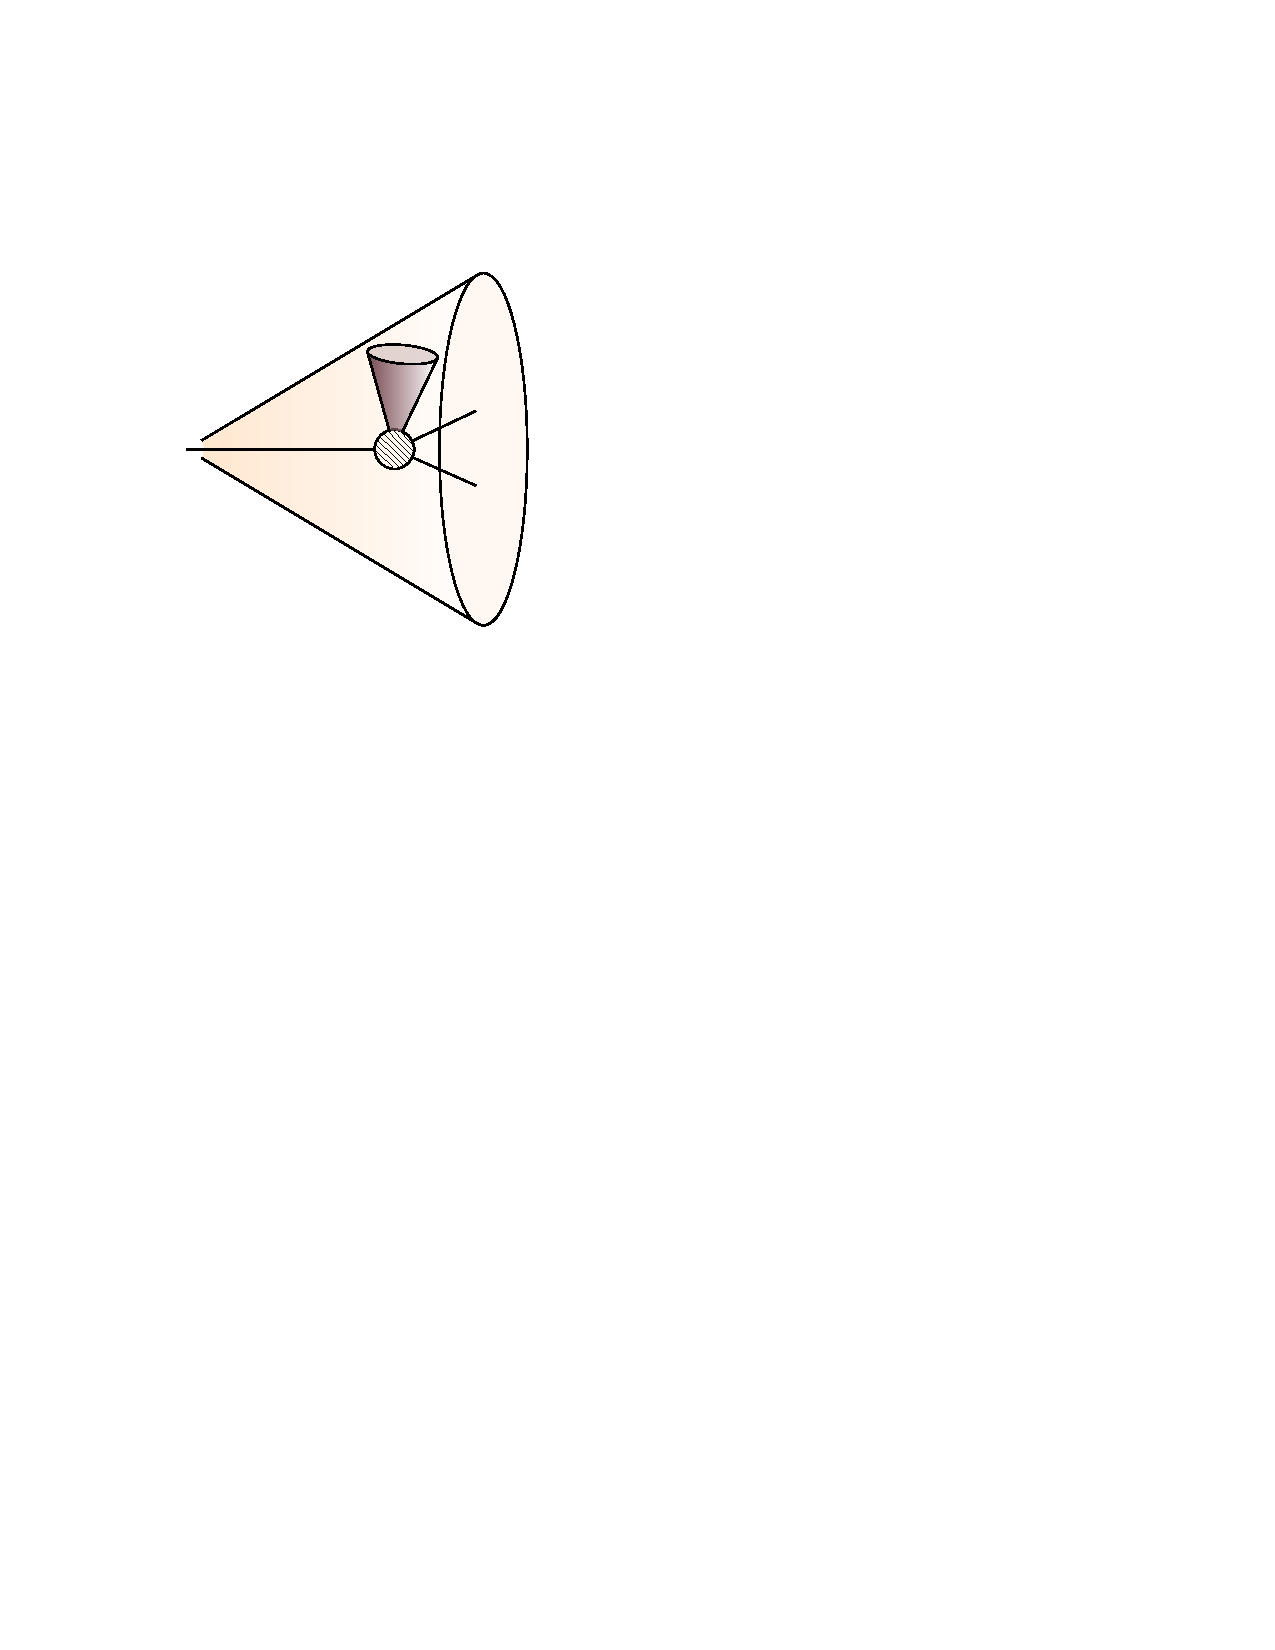
\includegraphics[width=.4\textwidth]{figures/misc/factorization/jet_fn_collinear_1.pdf}
        \label{fig:shower:cartoon:collinear1}
    }
    \hfill
    \subfloat[]{
        % Subfigure graphic
        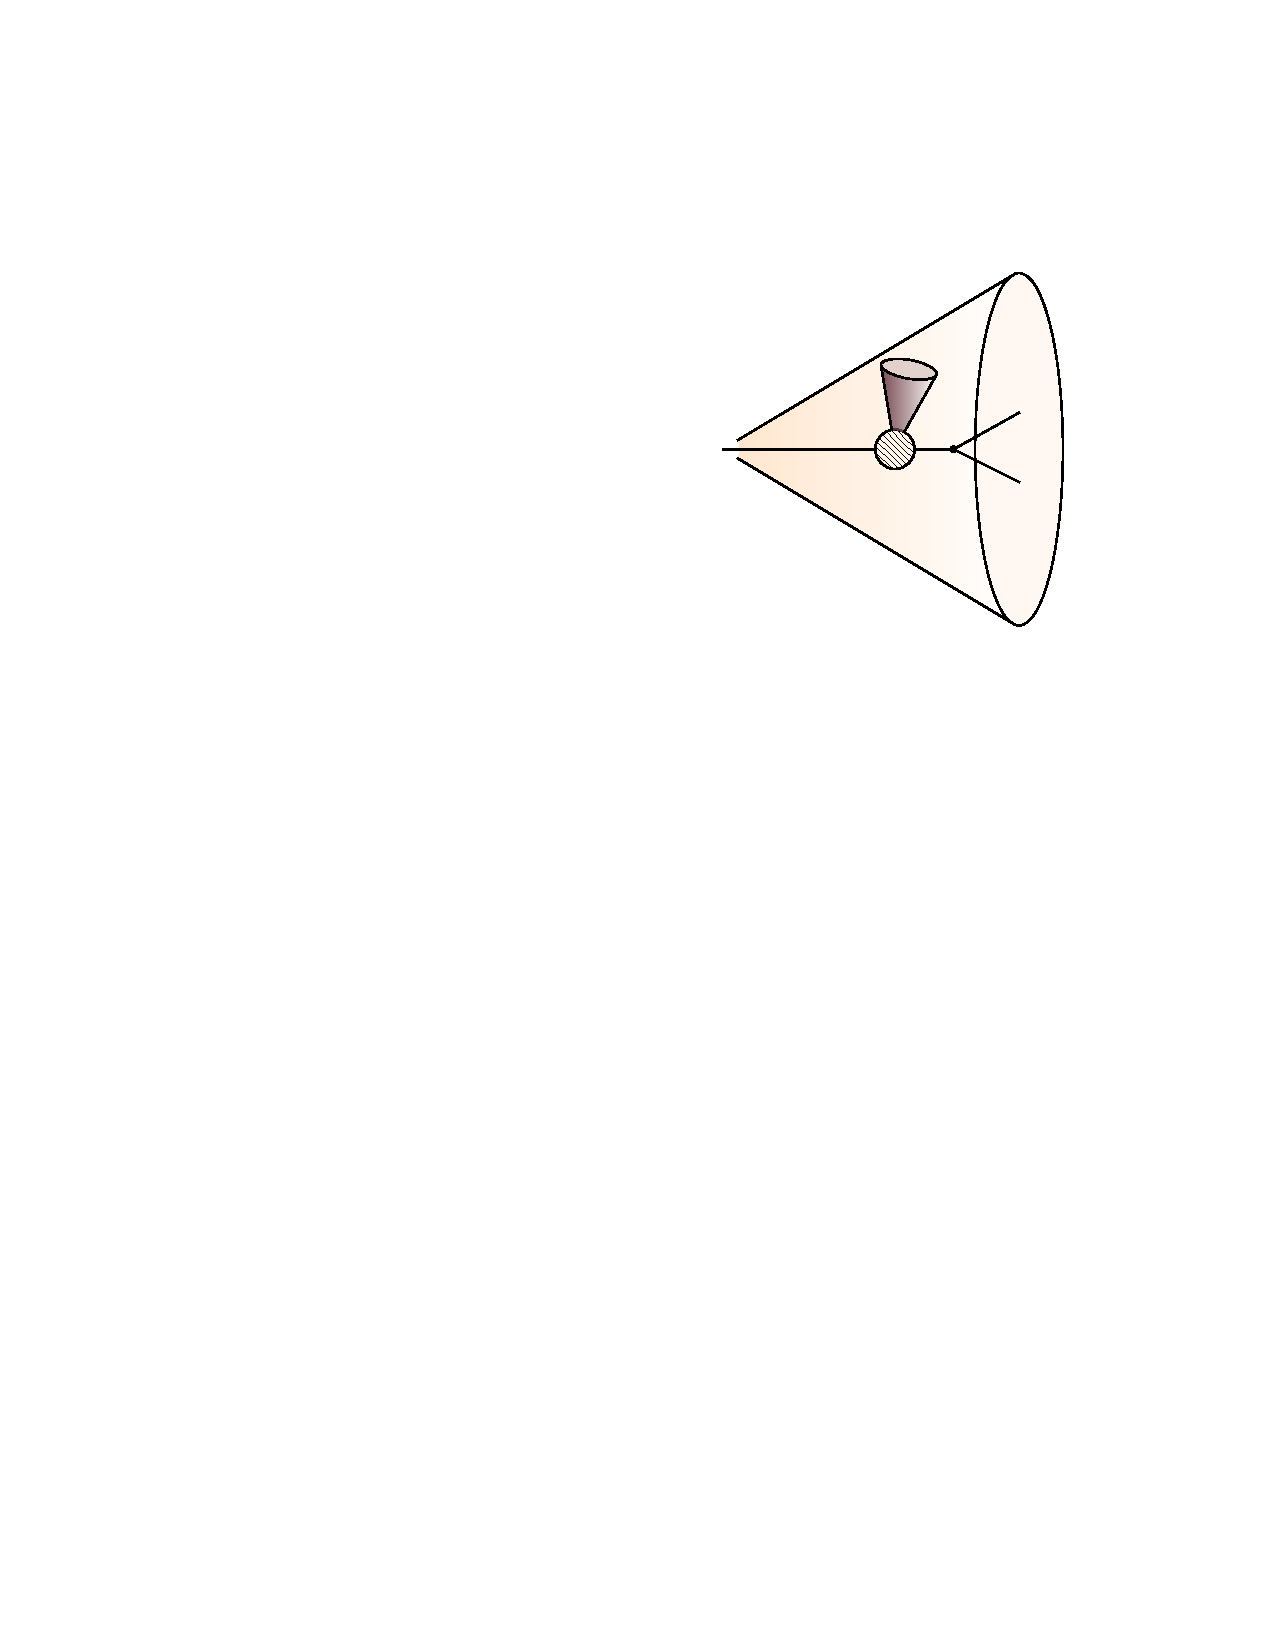
\includegraphics[width=.4\textwidth]{figures/misc/factorization/jet_fn_collinear_2.pdf}
        \label{fig:shower:cartoon:collinear2}
    }

    % Caption
    \caption[Depictions of jet function calculations for the EEC.]{
    Depictions of the calculational tools involved in computations of (jet functions for) \hyperref[fig:shower:cartoon:collinear1]{(a)} the EEC, and \hyperref[fig:shower:cartoon:collinear2]{(b)} the EEC in the collinear limit.
    %
    \hyperref[fig:shower:cartoon:collinear1]{(a)} depicts the fragmentation of an intiating parton into a pair of final-state particles, denoted as two outgoing lines, and additional inclusive radiation indicated by a large red cone.
    %
    \hyperref[fig:shower:cartoon:collinear2]{(b)} visualizes how the EEC in the collinear limit is dominated by pairs of final-state particles emerging from a single splitting;
    %
    in \hyperref[fig:shower:cartoon:collinear2]{(b)}, the fragmentation of the initiating parton produces wide-angle radiation which does not contribute to the EEC in the collinear limit.
    %
    The combination of partonic fragmentation and partonic splitting leads to a factorized expression for the EEC in the collinear limit, as in \Eq{eec_jet_fn_ll_1}.
    %
    \sam{fig capitalization}
    }
    \label{fig:shower:cartoon:collinear}
\end{figure}
% -----------------------------------

We will be most interested in the collinear limit of the EEC.
%
The collinear limit is useful in part because if we consider the contribution of a particular jet to the EEC in the context of factorization as discussed in Lemma~\ref{lem:eec-factorization}, the collinear limit is a valid tool as long as the jet itself is narrow.
%
Furthermore, the collinear limit simplifies our calculations by justifying the use of the collinear phase space measure and splitting functions of \Eqs{splitting_probability}{qcd_splitting_functions}.


To calculate the EEC in the collinear limit, we need only calculate the contributions due to the \emph{most} collinear pairs of particles in a jet;
%
since the fragmentation of the initiating parton is angular ordered (as discussed in \Sec{partonic-cascade}), the collinear limit of the EEC at LL is dominated by contributions of pairs of particles emerging from the final splittings in the jet (see \Fig{shower:cartoon:collinear}).

We conclude that the contribution of a single jet (or initiating parton) to the EEC in the collinear limit can be separated into two distinct, calculable pieces (see also \Fig{shower:cartoon:collinear2}):
\begin{enumerate}
    \item[a)]
    \textbf{The penultimate parton:}
    %
    parton-to-parton fragmentation produces one final intermediate/virtual parton \(f\) according to the partonic fragmentation functions \Eq{fragmentation_function}
    %
    (see also \Fig{shower:cartoon:fragmentation}).
    %
    We derived the relevant expressions for parton-to-parton fragmentation in \Sec{p2p-fragmentation}, where we found that the Mellin moments of parton-to-parton fragmentation functions were given by \Eq{ll_fragmentation_function}.
    %
    We repeat them here with \(\theta_f = 2\sqrt{\chi}\) (from \(\chi = (1-\cos\theta)/2, \theta\ll1\)) for convenience:
    \begin{align*}
        \hat{F}_{f \leftarrow i} (m;\,
        \theta_f = 2 \sqrt{\chi}\leftarrow \Rjet)
        =
        \le(
            \alpha_s\le(2\,Q\sqrt{\chi}\ri)
            \, / \,
            \alpha_s\le(Q\,\Rjet\ri)
        \ri)
        ^
        {\hat{p}(m) \, / \, 2\pi\beta_0}
        _{f\leftarrow i}
        ;
    \end{align*}

    \item[b)]
    \textbf{the final-state partons:}
    %
    the penultimate parton produces a pair of nearly collinear ``final-state'' partons, \(a\) and \(b\), according to the splitting functions \(P_{ab \leftarrow i}\) of \Eq{qcd_splitting_functions} and the pseudo-probability distribution of \Eq{splitting_probability}
    %
    (depicted schematically in \Fig{shower:cartoon:subjet_collinear}).
    %
    As we discuss below, the final states' angle \(\theta_{ab}\) and energy fractions \(x_a\), \(x_b\) determine their contribution \(C_{ab\leftarrow f}\) to the EEC:%
    \footnote{
        At LL, the \(C_{ab \leftarrow i}\) are independent of the energy of the hard process, \(Q\), and the energy fraction of the penultimate parton, \(x_f\).
        %
        At higher orders, the \(Q\) and \(x_f\) dependence of the \(C_{ab \leftarrow i}\) may be captured by the running of the coupling, \(\as \to \as\le(Q x_f x_a \theta_{ab}\ri)\), and also by higher order corrections to the splitting functions.
    }
    \begin{align}
        \label{eq:splitting_fn_contribution_to_eec}
        C_{ab\leftarrow f}(\chi)
        =
        \int \dd\mathbb{P}\le(x_a, \theta_{ab}\ri) \,
            x_a x_b
            \,
            \delta\le(\chi - \frac{1 - \cos\le(\theta_{ab}\ri)}{2}\ri)
        \approx
        \frac{2 \as}{\chi}
        \int_0^1 \dd x_a \, x_a (1-x_a) \,
        P_{ab \leftarrow f}(x_a)
        .
    \end{align}
\end{enumerate}

\remark{}{
    Of course, there is not \emph{really} such a thing as a final-state parton.
    %
    By ``final-state partons'', I mean ``partons which correspond to hadronic degrees of freedom exactly in the limit of infinite energy such that local-parton-hadron-duality is exact''.
    %
    However, even the ``final-state'' partons denoted \(a\) and \(b\) may undergo further splittings.
    %
    Nonetheless, due to strong angular ordering, these splittings do not affect the angle \(\theta_{ab}\) up to terms which are \emph{dramatically} smaller than \(\theta_{ab}\);
    %
    therefore, the function \(C_{ab\leftarrow f}(\chi)\) accurately captures the EEC up to small variations which vanish in the collinear limit, where \(\theta_{ab} = \chi \ll 1\).
}


Combining the physics of the fragmentation stage of jet formation with the final-state splittings we need in the collinear limit, we see that the contribution of the jet initiated by \(i\) to the EEC is
\begin{align}
    \label{eq:jet_fn_ll_0}
    \int_0^1
    \dd x_f
    \,
    F_{f \leftarrow i}\le(x_f;\,
    2 \sqrt{\chi}\leftarrow \Rjet\ri)
    \,
    x_f^2
    \,\,
    \sum_{ab} C_{ab\leftarrow f}\le(\chi\ri)
    =
    \hat{F}_{f \leftarrow i}
    \le(2;\,
    2 \sqrt{\chi}\leftarrow \Rjet\ri)
    \,\,
    \sum_{ab} C_{ab\leftarrow f}\le(\chi\ri)
    ,
\end{align}
%
where we have summed over final-state partons flavors, used the definition of the Mellin moment \(\hat{F}(2)\), and we use Einstein summation on the intermediate parton flavor \(f\).

Futhermore, since \Eq{jet_fn_ll_0} gives the (normalized) contribution of a narrow jet of partonic flavor \(i\) to the EEC in the collinear limit, it is precisely the jet function of \Eq{jet_fn_defn}.
%
Using \Eqss{ll_fragmentation_function}{splitting_fn_contribution_to_eec}{jet_fn_ll_0}, we can then write the LL jet function (EEC for a narrow jet of flavor \(i\)) as
\begin{align}
    \label{eq:eec_jet_fn_ll_1}
    J^i(\chi; \, Q)
    &=
    \frac{2 \as}{\chi}
    \,
    \sum_{a,b,\,f}
    \le(
        \int_0^1 \dd z \, z (1-z) \,
        P_{ab \leftarrow f}(z)
    \ri)
    \,
    \le(
        \frac{\alpha_s\le(2\,Q\sqrt{\chi}\ri)}
        {\alpha_s\le(Q\,\Rjet\ri)}
    \ri)
    ^
    {\frac{\hat{p}(m)}{2\pi\beta_0}}
    _{f\leftarrow i}
    .
\end{align}



Before proceeding to a phenomenological discussion of higher-point energy correlators, involving correlations of more than two final-state particles, we emphasize two important features of the jet function for the EEC:
\begin{itemize}
    \item
    the energy weighting of the EEC leads to the appearance of Mellin moments of fragmentation functions;

    \item
    The jet function inherits DGLAP evolution from the DGLAP evolution of \(F_{f \leftarrow i}\) in \Eq{fragmentation_dglap_upper}:
    \begin{align}
        \frac{\dd}{\dd\log\le(Q\,\Rjet\ri)}
        J^i\le(\chi;\, z,Q\ri)
        &=
        \frac{\alpha_s(Q\,\Rjet)}{\pi}
        \,\,
        \hat{p}(2)
        \,
        J^i\le(\chi;\, z,Q\ri)
    \end{align}
\end{itemize}
%
\Eq{jet_fn_ll_0} and these features of the resummed EEC have been well understood at least since the seminal work of \Reff{Konishi:1978dg,Konishi:1978yx}.





% ==============================================
\section{Efficient and Intuitive Higher Point Energy Correlators}
% ==============================================
\label{sec:new-angles}

Let us continue our exploration of energy-weighted correlators by defining and computing higher point (or $N$-point) energy correlators -- energy-weighted correlations of the energies of $N$ particles.
%
Recent work has highlighted the role of $N$-point energy correlators (ENCs) in precisely understanding the fundamental structure of particle interactions.
%
ENCs probe angular correlations between $N$ final-state particles, which offers a simple and intuitive way to separate physics at different scales and mitigate contamination from soft radiation.
%
Applications focused on the Large Hadron Collider (LHC) include the top quark mass \cite{Holguin:2022epo, Holguin:2023bjf, Holguin:2024tkz}, hadronization transition~\cite{Komiske:2022enw, Lee:2024esz}, dead-cone effect~\cite{Craft:2022kdo}, medium modifications in heavy-ion collisions~\cite{Andres:2022ovj, Andres:2023xwr, Barata:2023zqg, Andres:2023ymw, Singh:2024vwb, CMS:2024ovv, Bossi:2024qho}, and predictions for the energy flow of charged particles~\cite{Li:2021zcf, Chen:2022muj, Chen:2022pdu, Jaarsma:2023ell}.
%
Higher-point ENCs also yield more detailed shape information about the structure of radiation inside jets.
%
For example, recent work has leveraged the E3C to propose a new method for extracting the top quark mass from experimental data~\cite{Holguin:2022epo, Holguin:2023bjf, Holguin:2024tkz}.



In analogy to the EEC, we can define higher point correlators via
\begin{definitionbox}{\(N\)-point Energy Correlators}{enc}
    \emph{Higher Point Energy Correlators} are
    %
    An \vocab{\(N\)-point energy correlator} (E\(^N\)C, or ENC) is an energy-weighted angular correlation potentially depending on several variables.
    %
    As in the case of the EEC, we can write them in terms of differential cross sections:
    \begin{align}
        \label{eq:generalized-enc-event}
        \frac{\dd \Sigma}{\dd \chi_1\,\cdots\,\dd \chi_m}
        =
        \frac{1}{\sigma}
        \int \dd \sigma
        \sum_{\substack{\text{particles}\\i_1,\,\cdots,\,i_N}}
        \Bigg[
            &
            z_{i_1} \, \cdots z_{i_N}
            \,\,
            \delta\le(\chi_1 - f_1\le(\{\hat{n}\}\ri)\ri)
            \,\dots\,
            \delta\le(\chi_m - f_m\le(\{\hat{n}\}\ri)\ri)
        \Bigg]
        \,,
    \end{align}
    where the \(z_i\) indicate the energy or transverse momentum fraction of particle \(i\), \(\{\hat{n}\} = \{\hat{n}_{i_1},\,\dots,\,\hat{n}_{i_N}\}\) denotes the set of angular directions associated with the particles \(\{i_1,\,\dots,\,i_N\}\).
    %
    The \(f_1,\,\dots,\,f_m\) are all user-defined functions of the angular directions \(\{\hat{n}\}\), and parametrize the precise nature of the angular correlations probed by the ENC in question.
    %
    The choice of the \(\{f_\ell\}_{\ell=1}^{m}\) is therefore called the \vocab{parametrization} of the ENC.

\end{definitionbox}

\remark{}{
    ENCs in a theory with massless particles (or in the high energy limit) can be also be defined in terms of the energy flow operators of \Def{energy-flow} via
    \begin{align}
        \frac{\dd \Sigma}{\dd \chi_1\,\cdots\,\dd \chi_m}
        =
        \frac{1}{Q^N}
        \Big\langle
            \int \dd \Omega_1 \cdots \dd \Omega_N
            \,\,
            \mathcal{E}(\hat{n}_1)\,\cdots\,\mathcal{E}(\hat{n}_N)
            \,\,
            \delta\le(\chi_1 - f_1\le(\{\hat{n}\}\ri)\ri)
            \,\dots\,
            \delta\le(\chi_m - f_m\le(\{\hat{n}\}\ri)\ri)
        \Big\rangle
        \,,
    \end{align}
    where the expectation value indicates a quantum mechanical average, potentially over an ensemble of initial states, similarly to the expression of the EEC in terms of energy flow operators discussed in Remark~\ref{rem:eec-energyflow}.
}

\remark{}{
    In principle, the relative angular positions of \(N\) particles (e.g. as probed by an \(N\)-point energy correlator) can be completely determined through the knowledge of \(\binom{N}{2}\) independent coefficients -- the relative angular distance between each pair of particles -- up to an overall affine translation of the angular positions of each particle.
    %
    However, traditional parametrizations of $N$-point correlators over-determine the angular positions associated with a jet, leading to computational inefficiencies which we address below.
}


% ----------------------------------------------
\subsection{Projected Energy Correlators}
% ----------------------------------------------
\label{sec:enc-projected}

Projected Energy Correlators (\glspl{penc}) are $N$-point energy correlators which depend only on a single argument (i.e. in the language of \Eq{generalized-enc-event}, PENCs have \(m=1\)).
%
\glspl{penc} are the most commonly used $N$-point energy correlators due to their simplicity, but traditional parametrizations suffer from computational inefficiencies that prevent their calculation on realistic data sets.
%
We will first discuss the traditionally parametrized \glspl{penc} before addressing their computational inefficiencies with a new parametrization.

\begin{definitionbox}{Traditional PENC Parametrization}{}
    In proton-proton collisions -- the focus of this section -- \glspl{penc} are usually defined via~\cite{Chen:2020vvp}:
    \begin{align}
        \label{eq:old_def}
        \frac{1}{\sigma}\frac{\dd \sigma_N}{\dd R_L}
       \! =\!
        \biggl\langle
            \sum_{i_1 \dots i_N}
            z_{i_1} z_{i_2} \dots z_{i_N}
            \delta\big(
                R_L
                \!-\!
                \max_{k,\ell}
                \{R_{i_k,i_\ell}\}
            \big)
       \!\! \biggr\rangle.
    \end{align}
    %%%
    Here, $z_{i}= p_{T,i}/\sum_j p_{T,j}$ is the transverse momentum fraction carried by particle $i$ in the jet, $R_{i_k,i_\ell} = \sqrt{(y_{i_k,i_\ell})^2 + (\phi_{i_k,i_\ell})^2}$
    is the angular separation between particles $i_k$ and $i_\ell$ in the rapidity-azimuth plane, and the angular brackets indicate an expectation value over a sample of many hadronic jets.
    %
    The sum over $\{i_k\}_{k=1}^N$ indicates the sum over all sets of $N$ particles of a jet, and the variable \(R_L\) characterizes the maximum pairwise angular separation between the \(i_k\).
    %
    Notably, for $N>3$ the parametrization of ENCs in terms of the $R_{i_k,i_\ell}$ is over-complete:
    %
    the $R_{i_k,i_\ell}$ describe $N \choose 2$ distances, while only $2N-3$ are independent.
\end{definitionbox}

Unfortunately, the expression of \Eq{old_def} is computationally expensive due to the intricate phase space constraint \(R_L = \max_{k,\ell}\{R_{i_k,i_\ell}\}\).
%
For example, the time required to compute the (integer) \gls{penc} scales as $M^N/N!$ for a jet with $M$ particles; when analytically continued to non-integer values of $N$, the \gls{penc} suffers  a computational scaling of $2^{2M}$.%
%
\footnote{
    \textsc{FastEEC}~\cite{Budhraja:2024xiq} achieves a substantial speed up by replacing particles with subjets whose radius is chosen dynamically, depending on the desired level of angular resolution.
    %
    For non-integer $N$, \textsc{FastEEC} furthermore uses a recursive algorithm that reduces the standard $2^{2M}$ scaling down to $M\,2^M$~\cite{Budhraja:2024tev}.
}
%
This computational cost impedes several exciting \gls{penc} applications.
%
For example, \glspl{penc} have an approximate scaling behavior related to the $N$-th Mellin moment of the DGLAP splitting functions~\cite{Chen:2020vvp};
%
the analytic continuation of the \gls{penc} to non-integer $N$ therefore provides access both to the full splitting functions of QCD and, in the limit $N \to 0$, a unique opportunity to study small-$x$ physics and BFKL dynamics with jets~\cite{Chen:2020vvp, Budhraja:2024tev,Neill:2020bwv}.
%
At very large values of \(N\), \glspl{penc} also encode additional fundamental features of QCD~\cite{Chen:2020vvp,Dai:2024wff}, such as level crossings with twist-4 operators.
%
Furthermore, in the high-multiplicity environment of heavy ion collisions, even computing \glspl{penc} for \(N=3\) has been computationally challenging, limiting their potential in studying medium effects~\cite{Bossi:2024qho}.
%
Improved computational efficiency is therefore necessary to leverage the full potential of \glspl{penc} in the study of realistic data samples.


Therefore, rather than focusing on the traditional projections of ENCs, in this section we focus on new parameterizations of higher point energy correlators, introduced in \Reff{}, with a number of improved properties.
%
First, our parametrization of the \gls{penc} depends on the largest distance \(R_1\) to a ``special'' particle $s$ in a set of $N$ particles, suitably averaged over all choices for $s$;
%
this yields simpler phase space restrictions than the traditional parametrization for the \gls{penc} in terms of the largest pairwise angle~\cite{Chen:2020vvp}.
%
Second, when considering more differential information, our parametrization of resolved ENCs (\gls{renc}s) employs non-redundant polar coordinates centered around the special particle, as in \Fig{cartoon}, yielding intuitive visualizations of jet substructure.
%
This differs from the traditional approach, which uses over-complete information from the set of all pairwise distances and neglects information about the relative orientation of particles.
%
Third, our parametrization offers dramatic improvements in computational performance, which is essential for their use in experimental analyses.
%
Finally, we anticipate that these conceptual and computational improvements will yield simpler theoretical calculations.
%
Our implementation for computing the \glspl{penc} of \Eq{new_def} be found on GitHub as an update to \textsc{FastEEC}~\cite{FASTEEC}, and of our \glspl{penc} and \gls{renc}s at \texttt{ResolvedEnergyCorrelators}~\cite{github:RENC}.


\begin{figure}
    \centering
    \scalebox{1.2}{
        \begin{tikzpicture}
% Defining colors
\definecolor{cornflowerblue}{rgb}{0.39, 0.58, 0.93}
\definecolor{azure(colorwheel)}{rgb}{0.0, 0.5, 1.0}

\definecolor{coralred}{rgb}{1.0, 0.25, 0.25}
\definecolor{cadmiumorange}{rgb}{0.93, 0.53, 0.18}
\definecolor{darkgoldenrod}{rgb}{0.72, 0.53, 0.04}

\definecolor{rosevale}{rgb}{0.67, 0.31, 0.32}
\definecolor{palebrown}{rgb}{0.6, 0.46, 0.33}

\definecolor{mediumorchid}{rgb}{0.73, 0.33, 0.83}

\definecolor{ao}{rgb}{0.0, 0.5, 0.0}
\definecolor{lightseagreen}{rgb}{0.13, 0.7, 0.67}

% Defining colors associated with different nodes
\colorlet{colsp}{ao}
\colorlet{coli1}{cornflowerblue}
\colorlet{coli2}{coralred}
\colorlet{coli3}{mediumorchid}
\colorlet{coliN}{palebrown}

% All grey
% \colorlet{colsp}{gray}
% \colorlet{coli1}{gray}
% \colorlet{coli2}{gray}
% \colorlet{coli3}{gray}
% \colorlet{coliN}{gray}



% =:=:=:=:=:=:=:=:=:=:=:=:=:=:=:=:=:=:=
% Particle N
% =:=:=:=:=:=:=:=:=:=:=:=:=:=:=:=:=:=:=
% Beginning here so it is on the back layer
\draw[color=coliN, line width=0.5mm]
    (0, 0) -- (120:1.0) coordinate (iN)
    node[pos=0.4, left, text=black, font=\Large]
    {\textcolor{coliN!50!black}{$\boldsymbol{R_{N-1}}$}};

\newif\ifrecursive
\recursivefalse
\ifrecursive
% Sketch of N-1
\draw[color=gray, dashed, line width=0.5mm]
    (0, 0) -- (75:1.6) coordinate (iNm)
    node[pos=0.4, left, text=black, font=\Large] {};
% iN-1 node
\filldraw[color=gray]
    (iNm) circle (3pt)
    node[above, xshift=-5pt, yshift=2pt]
    {\textcolor{gray!60!black}{$i_{N-2}$}};
% phi_N arc
\draw[-stealth, color=coliN, dashed, line width=0.4mm]
    (75:1.0)
    arc[start angle=75, end angle=115, radius=1.0]
    node[pos=0.55, above, text=black, font=\large]
    {\textcolor{coliN!50!black}{$\phi_{N-1}$}};
\else
% phi_N arc
\draw[-stealth, color=coliN, dashed, line width=0.4mm]
    (0:1.0)
    arc[start angle=0, end angle=115, radius=1.0]
    node[pos=0.55, above, text=black, font=\large]
    {\textcolor{coliN!50!black}{$\phi_{N-1}$}};
\fi

% iN node
\filldraw[color=coliN!50!black]
    (iN) circle (3pt)
    node[above left, xshift=-2pt, yshift=-2pt, font=\large]
    {\textcolor{coliN!50!black}{$i_{N-1}$}};

% =:=:=:=:=:=:=:=:=:=:=:=:=:=:=:=:=:=:=
% Particle 1
% =:=:=:=:=:=:=:=:=:=:=:=:=:=:=:=:=:=:=
\draw[color=coli1, line width=0.5mm]
    (0, 0) -- (0:5) coordinate (i1)
    node[pos=0.6, below, sloped, text=black,
         font=\Large]
        {\textcolor{coli1!50!black}{$\boldsymbol{R_1}$}};

% i1 node
\filldraw[color=coli1!50!black]
    (i1) circle (3pt)
    node[below right, font=\large]
    {\textcolor{coli1!50!black}{$i_1$}};

% =:=:=:=:=:=:=:=:=:=:=:=:=:=:=:=:=:=:=
% Particle 2
% =:=:=:=:=:=:=:=:=:=:=:=:=:=:=:=:=:=:=
\draw[color=coli2, line width=0.5mm]
    (0, 0) -- (50:4.5) coordinate (i2)
    node[pos=0.6, left, text=black, xshift=-4pt, font=\Large]
    {\textcolor{coli2!50!black}{$\boldsymbol{R_2}$}};

% phi_2 arc
\draw[-stealth, color=coli2, dashed, line width=0.4mm]
    (0:4.5)
    arc [start angle=0, end angle=48.5, radius=4.5]
    node[pos=0.5, right, text=black, font=\large]
    {\textcolor{coli2!50!black}{$\phi_2$}};

% i2 node
\filldraw[coli2!50!black]
    (i2) circle (3pt)
    node[below, yshift=-5pt, font=\large]
    {\textcolor{coli2!50!black}{$i_2$}};


% =:=:=:=:=:=:=:=:=:=:=:=:=:=:=:=:=:=:=
% Particle 3
% =:=:=:=:=:=:=:=:=:=:=:=:=:=:=:=:=:=:=
\draw[color=coli3, line width=0.5mm]
    (0, 0) -- (30:3) coordinate (i3)
    node[pos=0.6, below, text=black, xshift=9pt, font=\Large]
    {\textcolor{coli3!50!black}{$\boldsymbol{R_3}$}};

\ifrecursive
% phi_3 arc
\draw[-stealth, color=coli3, dashed, line width=0.4mm]
    (50:3.0)
    arc [start angle=50, end angle=32, radius=3.0]
    node[pos=0.3, right, xshift=2pt, text=black, font=\large]
    {\textcolor{coli3!50!black}{$-\phi_3$}};
\else
% phi_3 arc
\draw[-stealth, color=coli3, dashed, line width=0.4mm]
    (0:3.0)
    arc [start angle=0, end angle=28, radius=3.0]
    node[pos=0.5, right, text=black, font=\large]
    {\textcolor{coli3!50!black}{$-\phi_3$}};
\fi

% i3 node
\filldraw[color=coli3!50!black]
    (i3) circle (3pt)
    node[below, yshift=-5pt, font=\large]
    {\textcolor{coli3!50!black}{$i_3$}};




% =:=:=:=:=:=:=:=:=:=:=:=:=:=:=:=:=:=:=
% Draw the central point s
% =:=:=:=:=:=:=:=:=:=:=:=:=:=:=:=:=:=:=
\filldraw[color=colsp!50!black]
    (0, 0) circle (3pt)
    node[below, yshift=-5pt, xshift=-2pt, font=\Large]
    {\textcolor{colsp!50!black}{$s$}};


% =:=:=:=:=:=:=:=:=:=:=:=:=:=:=:=:=:=:=
% Draw ellipses to indicate missing points
% =:=:=:=:=:=:=:=:=:=:=:=:=:=:=:=:=:=:=
\draw[gray, dotted, line width=0.4mm,
      xshift=-0.00cm, yshift=0.50cm]
      (55:3.6)
    arc[start angle=103, end angle=150, radius=4.]
    node[pos=0.55, sloped, above,
         xshift=0.1cm, yshift=0.2cm, text=black]
        {$R_{N-1} < \cdots < R_2 < R_1$};

\end{tikzpicture}

    }
    \caption[Cartoon of the new parameterization of ENCs introduced by the author and collaborators]{
        A cartoon of the new parametrization of ENCs we introduce in \Eqs{new_def}{renc}.
        %
        Instead of computing the ENC using all \(\binom{N}{2}\) pairwise distances, we parametrize the ENC with \(2N - 3\) oriented polar coordinates centered on a special particle \izero{}, and then perform a momentum-weighted sum over all choices for \izero{}.
    }
	\label{fig:cartoon}
\end{figure}


\begin{definitionbox}{New PENC Parametrization}{}
    Our new parametrization of \glspl{penc}, with a simpler phase space structure, takes the form:
    %%%
    \begin{align}
        \label{eq:new_def}
        \frac{\dd \Sigma_\text{PENC}}{\dd R_1}
        :=
        \frac{1}{\sigma}\frac{\dd \sigma_N}{\dd R_1}
        &=
        \biggl\langle
            \sum_{\izero=1}^M  z_{\izero} \!\!
            \sum_{i_1 \dots i_{N-1}}
           \!\! z_{i_1} \dots z_{i_{N-1}}
            \delta (
                R_1
                \!-\!
                \max_j\{R_{\izero,i_j}\}
            ) \!
        \biggr\rangle ,
        \notag \\
        &=: \text{PENC}(R_1) \,
        .
    \end{align}
    %%%
    %
    The sums on \(\izero\) and \(\{i_j\}_{j=1}^{N-1}\) again run over all $M$ particles within a jet.
    %
    The crucial simplification is that our \gls{penc} is based on a new variable, \(R_1\), that indicates the maximum distance \(\max\{R_{\izero, i_j}\}\) between the \textit{single} particle \(\izero\) and any of the remaining $N-1$ particles \(\{i_j\}_{j=1}^{N-1}\).
\end{definitionbox}


\begin{figure}
    \centering
    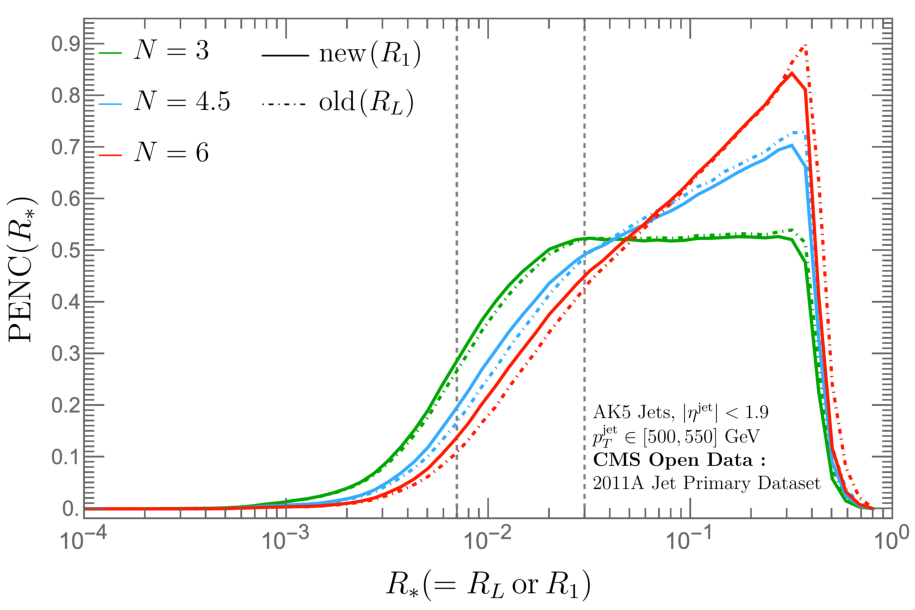
\includegraphics[width=0.8\textwidth]{figures/eec-angles/ENC.pdf}
    \caption[%
        Comparisons of the new and traditional parameterizations of projected ENCs.
        %
        Figure by Ankita Budhraja.
    ]{
        \gls{penc} distributions for $N \in \{3, 4.5, 6\}$, calculated using our new parametrization (solid) and the traditional parametrization (dashed).
        %
        $R_{*}$ denotes the largest distance to the special particle for our new parametrization ($R_1$), and the largest separation between the $N$ particles for the traditional one ($R_L$).
        %
        The differences are small in the perturbative region $R_{*} \!\! \gg  \! \Lambda_{\rm QCD} /p_T$, but become noticeable in the transition between perturbative and non-perturbative regimes (indicated by the vertical dashed lines).
        %
        Figure by Ankita Budhraja.
    }
	\label{fig:ENC}%
\end{figure}

\indent
Like the old variable \(R_L\) of \Eq{old_def}, \(R_1\) still roughly characterizes the maximum angular scale between a set of \(N\) particles, since \(R_L/2 \leq R_1 \leq R_L\) by the triangle inequality.
%
Indeed, the \glspl{penc} displayed in \Fig{ENC} show that the difference between our parametrization and that of \Eq{old_def} is small, and that both parametrizations have similar scaling behavior in the perturbative region (though there are some differences in the perturbative to non-perturbative transition).
%
\Figss{ENC}{bullseye}{density} all feature energy correlators evaluated on the CMS 2011A Jet Primary Dataset~\cite{CERNOpenDataPortal, CMS:JetPrimary2011A}, also available in MIT Open Data format~\cite{Komiske:2019jim, komiske_patrick_2019_3340205}, on jets with transverse momenta $p_{T}^{\text{jet}} \in [500, 550]$ GeV and pseudo-rapidity $\vert \eta^{\rm jet} \vert < 1.9$.

\indent
A major strength of the parameterization of \Eq{new_def} it its dramatically improved computational efficiency relative to older \gls{penc} paramterization.
%
The computational efficiency of our parametrization is more clear in the expression for (normalized) cumulative distribution:
%%%
\begin{align} \label{eq:new_cml}
  \Sigma_N(R_1)
  \!
  &=
  \!
  \frac{1}{\sigma}
  \int_0^{R_1}
  \!\!
  \dd R_1'
  \,
  \frac{\dd \sigma_N}{\dd R_1'}
   % \notag \\
  =
  % \!
  \biggl\langle \sum_{\izero} z_{\izero} [z_{\rm disk}(\izero,R_1)]^{N-1}
  \biggr\rangle
  ,
\end{align}
%%%
where $z_{\rm disk}(\izero,R_1)$ denotes the total transverse momentum fraction of all particles within a radius $R_1$ of the special particle \izero{}.
%
Notably, the simple form of \Eq{new_cml} holds even for non-integer $N$.
%
A practical way to evaluate \Eq{new_cml} (and \Eq{new_def} after differentiation) is, for each $\izero$, to first sort all particles by their distance with respect to $\izero$, and then to compute $\Sigma_N(R_1)$ by beginning with $R_1=0$ and then increasing it.
%
Sorting particles by their distance to \izero{} takes $M\ln M$ time, and the remaining sum over \izero{} scales with $M$, resulting in an overall computation time scaling as $M^2 \ln M$.
%
This computational speed up is especially interesting for heavy-ion collisions where $M$ is typically very large.


The factorization formula in \Eq{factorization_defn} can be extended to that of traditionally-parameterized \glspl{penc}~\cite{Chen:2020vvp}.
%
The factorization for existing \glspl{penc} also applies to our new parameterization, with one small difference:
%
because the variables $R_1$ and $R_L$ differ for three or more emissions, the jet function for our \glspl{penc} differs from the old one at $\ord{\alpha_s^2}$, or at next-to-next-to-leading logarithmic accuracy (NNLL).
%
In \Prob{nll_equiv}, we discuss how the NLL equivalence of jet functions implies that $
    \Sigma_N
    (R_L)
    =
    \Sigma_N(
    R_1 = R_L[
        1
        +
        \mathcal{O}
        (
        \alpha_s
        )
    ]
    )
$%
.
%
Furthermore, at NNLL and beyond, we expect that the simple dependence of \Eq{new_cml} on $N$ will substantially simplify the calculation of the jet function for $R_1$.
%
By contrast, the jet function using the old parametrization requires dedicated calculations for each individual value of $N$~\cite{Dixon:2019uzg,Chen:2023zlx}.




\remark{}{
    The cumulative distribution associated with our new \gls{penc} parametrization, given in \Eq{new_cml}, is the $N$-th Mellin moment in $z$ of
    %%%
    \begin{align}
        \frac{1}{\sigma}
        \frac{\dd \sigma}{\dd z}
        (R_1)
        =
        \Bigl
        \langle\sum_{\izero} z_{\izero}\, \delta
        \bigl[
            z
            -
            z_{\rm disk}(\izero,R_1)
        \bigr]
        \Bigr\rangle
        \,,
    \end{align}
    %%%
    which is also the differential jet rate in a ``jets-without-jets approach'' if \(R_1\) is treated as a jet radius~\cite{Bertolini:2013iqa,Bertolini:2015pka}.
    %
    A similar moment relation between the jet rate and the original ENC was noted in Ref.~\cite{Lee:2024icn}.
}





% ----------------------------------------------
\subsection{Resolved Energy Correlators}
% ----------------------------------------------
\label{sec:enc-resolved}

By including (or \emph{resolving}) more detailed angular information about the positions and relative orientations of particles within the jet, we may generalize our new parametrization for the \gls{penc} to introduce the \gls{renc}:


\begin{definitionbox}{Resolved Energy Correlator (RENC)}{renc}

    \vocab{\glslink{renc}{Resolved Energy Correlators (RENCs)}} are defined as the correlators

    \begin{align}
        \label{eq:renc}
        &\text{RENC}(R_1, R_2, \phi_2, R_3, \phi_3, \dots)
        := \frac{1}{\sigma}
        \frac{\dd \sigma_N}{\dd R_1 \dd R_2 \dd \phi_2 \dd R_3 \dd \phi_3 \dots} \notag
        \\
        &
        = \biggl\langle
        \sum_{\izero}
        z_{\izero}
        \!\!
        \sum_{i_1 \geq\dots\geq i_{N-1}}
        \!\!\!\!
        z_{i_1} \dots z_{i_{N-1}}
        \binom{N}{n_1\,n_2\, \dots}\,
        \delta
            (R_1 \!-\! R_{\izero,i_1}
        )
        \notag
        \\
        & \qquad\qquad\qquad\qquad
        \ \times
        \rho_{i_2}(R_2,\phi_2)\, \rho_{i_3}(R_3,\phi_3)\, \dots\biggr\rangle
        \, ,
    \end{align}
    %%%
    where for each $s$, the $i_j$ are indexed such that $R_{s,i_1} \ge R_{s,i_2} \ge \ldots$, and the summand involves the per-particle densities:
    %%%
    \begin{align}
        \rho_{i_j}(R_j, \phi_j)
        =
        \delta(
            R_j
            -
            R_{\izero,i_j}
        )\,
        \delta(
            \phi_j
            -
            \phi_{i_{j-1},i_j}
        )
    \,.\end{align}
    %%%
    The ``$\dots$" correspond to additional  \(R_j\) and \(\phi_j\), and $n_k$ denotes how often particle $k$ of the jet appears among the $i_j$ (such that terms with $n_k>1$ encode self-correlations of particle $k$), with $\sum^M_{k=1} n_k = N$.

\end{definitionbox}


\begin{figure}
    \centering
    \subfloat[]{
    	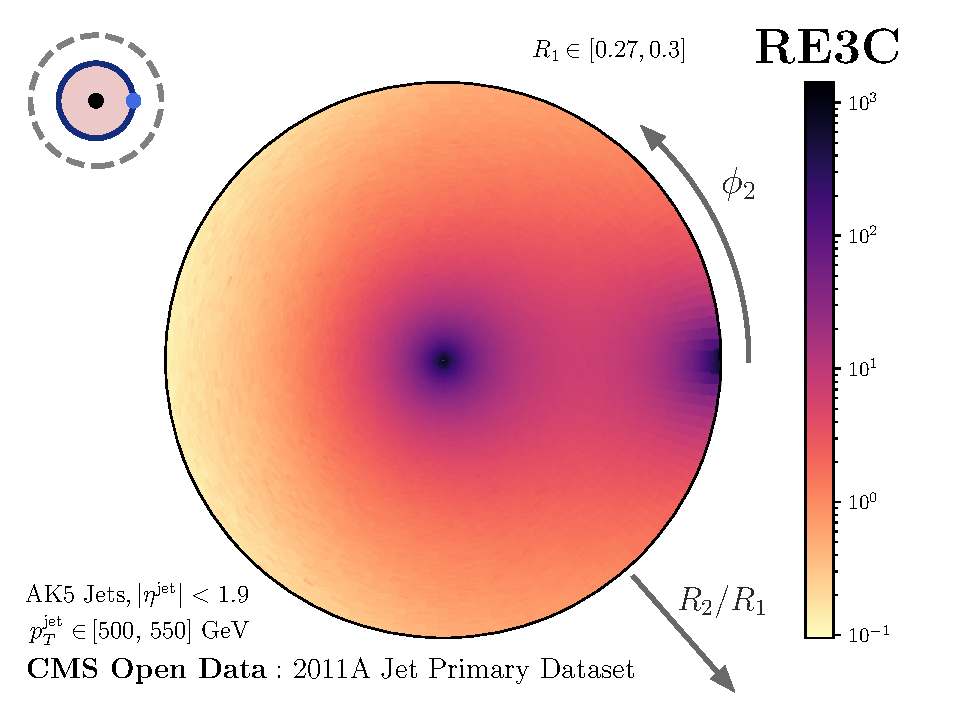
\includegraphics[width=0.33\textwidth]{figures/eec-angles/opendata/od_3particle_bullseye_0.286592.pdf}
        \label{fig:bullseye_new}
     }
     \subfloat[]{
    	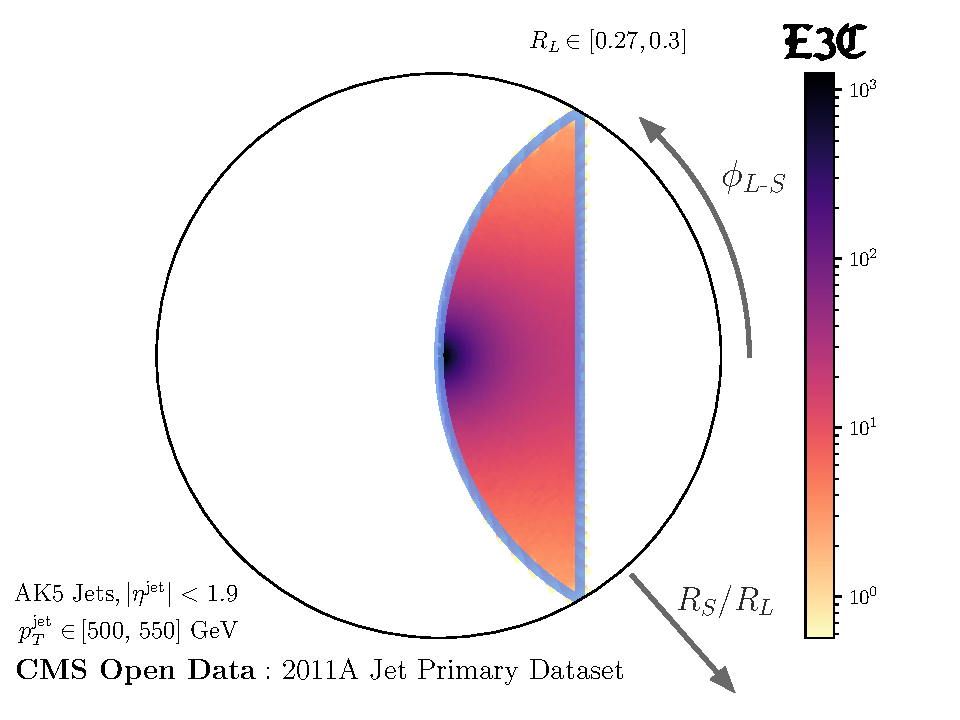
\includegraphics[width=0.33\textwidth]{figures/eec-angles/opendata/od_3particle_old_bullseye_0.286592.pdf}
        \label{fig:bullseye_old}
     }
    \subfloat[]{
    	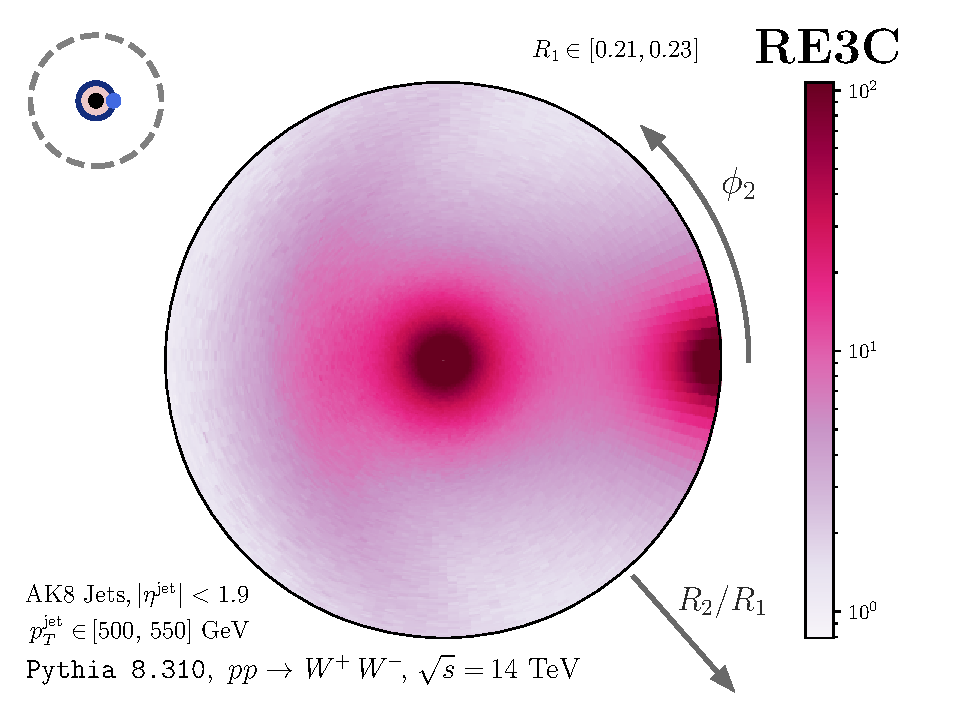
\includegraphics
        [width=0.33\textwidth]
        {figures/eec-angles/supplemental/3particle/w0.216087_3particle_bullseye.pdf}
        \label{fig:bullseye_new_w}
    }
    \caption[Polar heat maps of three-point energy correlators.]{
        Polar heat maps visualizing \textbf{(a)} our new RE3C applied to CMS Open Data, \textbf{(b)} the traditional E3C applied to CMS Open Data, and \textbf{(c)} our new parametrization applied to $W$-boson-initiated jets from \texttt{Pythia 8.310}.
        %
        In \textbf{(a)} and \textbf{(c)}, the radial variables correspond to \(R_2/R_1\), the polar angle corresponds to \(\phi_2\), and we show the RE3C in the bin $R_1 \in [0.27,0.3]$.
        %
        In \textbf{(b)} the radius corresponds to \(R_S/R_L\), the polar angle corresponds to the angle between associated lines of length \(R_S\) and \(R_L\), and we show the E3C in the bin $R_L \in [0.27,0.3]$.
        %
        In all three plots, we see collinear enhancements for the RE3C near the origin, when two particles become very close in angle.
        %
        In \textbf{(a)} and \textbf{(c)}, we also see collinear enhancements as \(R_2/R_1 \to 1\) and \(\phi_2 \to 0\), and \textbf{(c)} exhibits additional non-collinear enhancements correlated with the \(W\)-boson mass.
    }
	\label{fig:bullseye}%
\end{figure}



\begin{figure}
\centering
    \subfloat[]{
        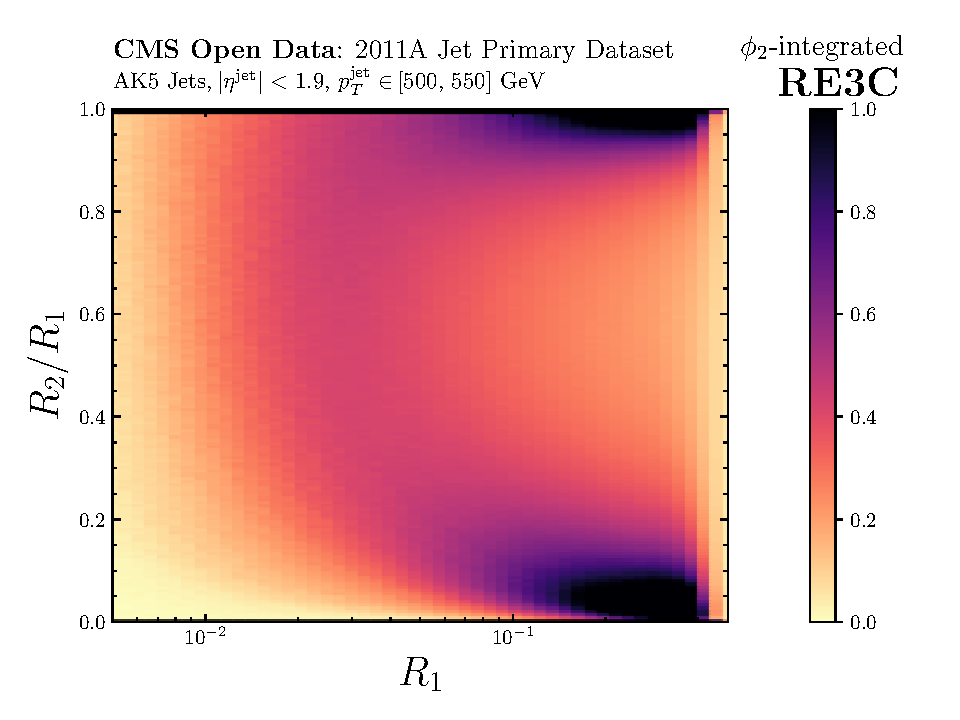
\includegraphics
        [width=0.33\textwidth]{figures/eec-angles/od_newdef_density.pdf}
    	\label{fig:density_new}%
    }
    \subfloat[]{
        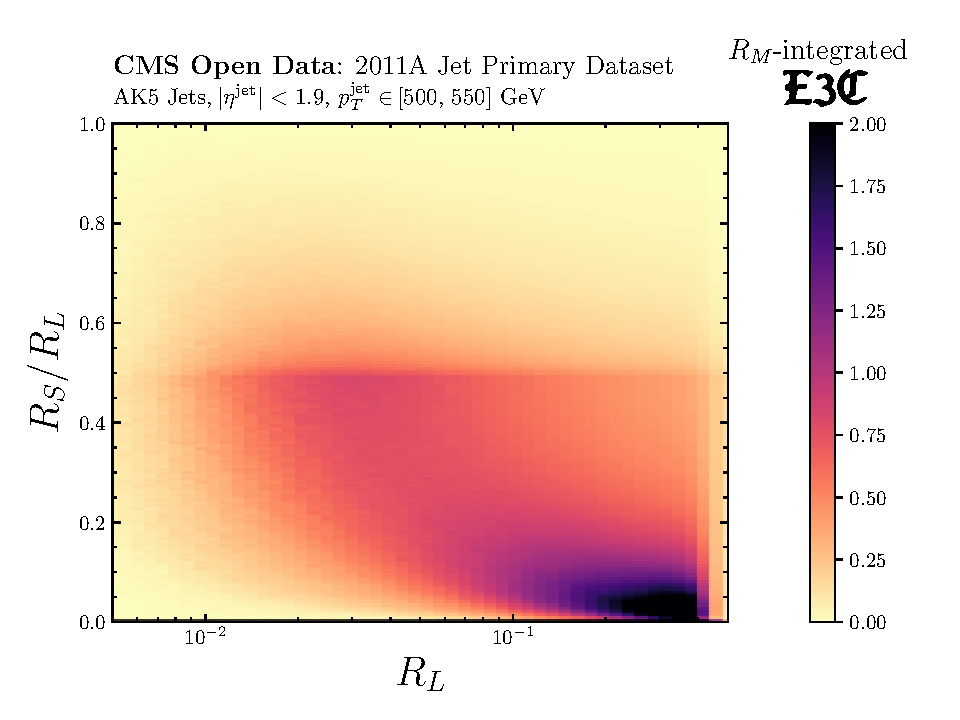
\includegraphics
        [width=0.33\textwidth]
        {figures/eec-angles/od_olddef_density.pdf}
    	\label{fig:density_old}%
    }
    \subfloat[]{
        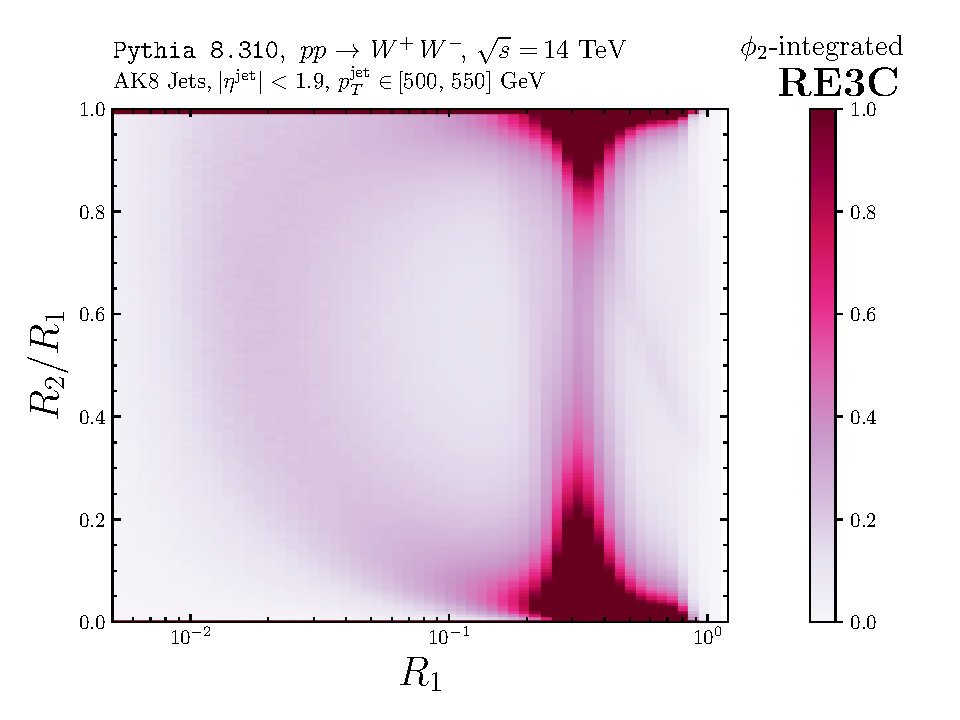
\includegraphics
        [width=0.33\textwidth]
        {figures/eec-angles/supplemental/density/w_newdef_density.pdf}
    	\label{fig:density_w}%
    }
    \caption[Three-point energy correlators integrated over azimuthal angle.]{
        Normalized distributions \textbf{(a)} our new RE3C applied to CMS Open Data when integrated over the azimuthal angle \(\phi_2\), \textbf{(b)} the traditional E3C applied to CMS Open Data integrated over the intermediate angle $R_M$ (analogous to integrating over \(\phi_s\)), and \textbf{(c)} our new, \(\phi_2\)-integrated RE3C applied to $W$-boson-initiated jets.
    }
	\label{fig:density}%
\end{figure}





Our parametrization is visualized in \Fig{cartoon}, and utilizes polar coordinates around $\izero$, ordered in radius $R_1 \! > \! R_2 \! > \! \dots$ and with an \emph{oriented} azimuthal angle $\phi_j$ taken relative to the $(j\!-\!1)$-th resolved emission.
%
The \(R_j\) and \(\phi_j\) use \(2N-3\) variables to completely characterize the positions of all particles in the jet, relative to the axis defined by particles \(s\) and \(i_1\).
%
The multinomial coefficient in \Eq{renc} arises due to the ordering of the \(R_j\), and accounts for the possibility that two or more of the $i_j$ may be equal.
%
Integrating inclusively over $\{R_j, \phi_j\}_{j=2}^{N}$ (which sets the third line of \Eq{renc} to unity) reduces the \gls{renc} to the \gls{penc} from \Eq{new_def}.


The \glspl{renc} we introduce also preserve information about relative orientations, whereas even in the simple example of $N=3$, the traditional E3C parametrization in terms of the largest ($R_L$), medium ($R_M$), and shortest ($R_S$) distances does not.
%
We visualize the additional orientation information preserved by our RE3Cs in \Figs{bullseye_new}{bullseye_old}, where we compare polar heat maps of our parametrization of the RE3C to the traditional paramterization of the E3C.
%
The additional angular information carried by our new RE3C also leads to striking visual differences when comparing jets initiated by different processes.
%
For example, the unique characteristics of the RE3C evaluated on $W$-boson initiated jets generated with \texttt{Pythia 8.310}, shown in \Fig{bullseye_new_w}, clearly distinguish it from the RE3C of QCD-initiated jets.
%
This qualitative difference is not visible in the traditional parametrization, as shown in the supplemental material together with similar visualizations for additional processes.


We also note that each additional resolved particle (i.e.\ each \((R_j, \phi_j)\) pair) introduces a factor of $M$ to the scaling of the \gls{renc} computation time.
%
In contrast, the computation time for e.g.~the traditional 4-point correlator scales as $M^4$ independent of how many angles were resolved.


In \Fig{runtime}, we display the computational runtime of our code for the evaluation of \glspl{penc} and \glspl{renc} on jet samples from CMS Open Data.
%
\Fig{runtime_scaling} shows how the scaling time for each nearly follows an \(M^r\) scaling, where \(r\) indicates the number of resolved emissions.
%
Furthermore, the independence of the runtime on the value of \(N\) allows us to compute the \gls{penc} for enormous, and previously unimaginable, values of \(N\);
%
some examples up to \(N = 100\) are shown in \Fig{runtime_largeN}.
%
We highlight that our implementation takes similar runtime for all values of $N$.
%
Therefore, we expect the \gls{penc} we introduce in this work to significantly benefit ongoing studies which apply energy correlators in jets produced in heavy-ion collisions for revealing the emergent scales of the quark-gluon plasma in these environments.

\begin{figure}[t!]
    % \centering
    \subfloat[]{
        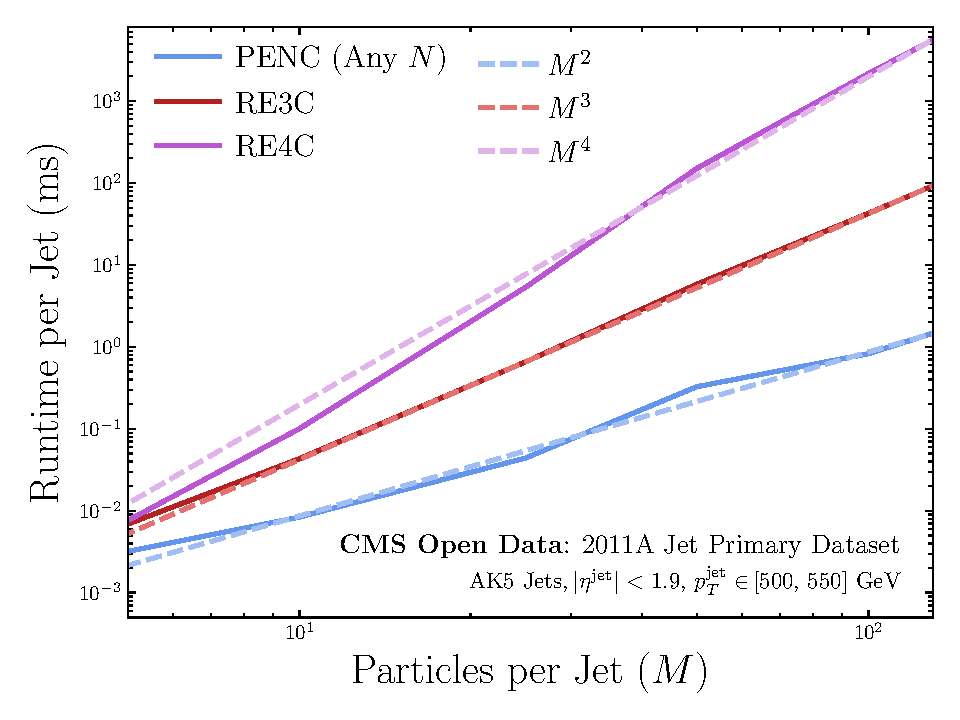
\includegraphics[width=.45\textwidth]{figures/eec-angles/opendata/opendata_runtimes_fewM.pdf}
        \label{fig:runtime_scaling}
    }
    $\qquad$
    \subfloat[]{
        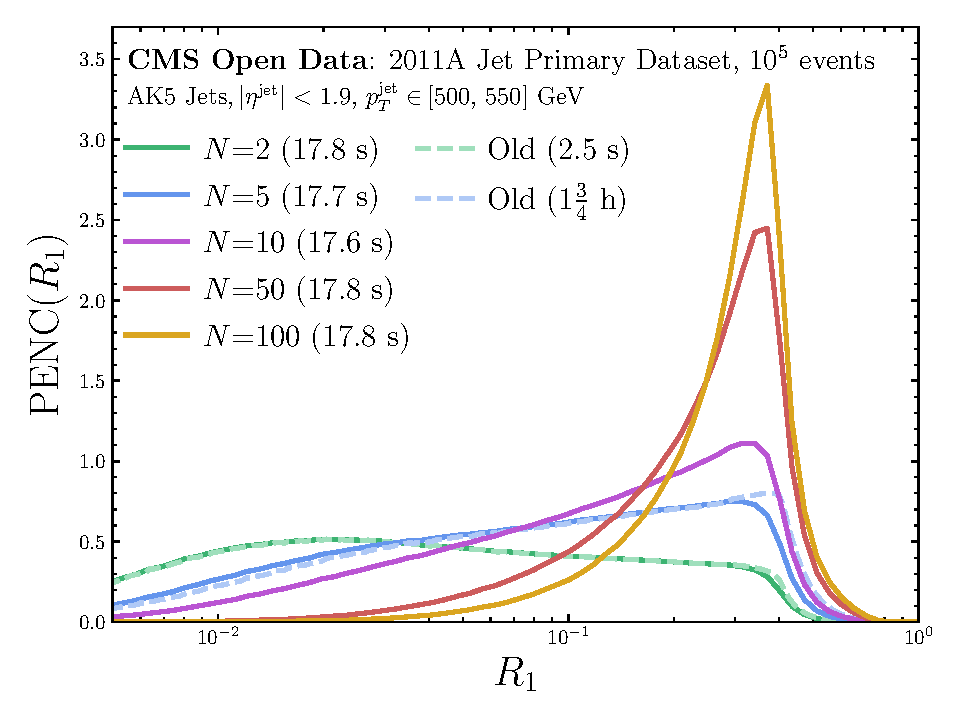
\includegraphics[width=.45\textwidth]{figures/eec-angles/opendata/od_projected_runtime.pdf}
        \label{fig:runtime_largeN}
    }
    \caption[Plots emphasizing the computational performance of the new parameterization of energy correlators discussed in this work.]
    {
        Plots emphasizing the computational performance of the energy correlators we introduce in this work.
        %
        \sam{fix, together wtih the other ref comments}
        %
        \textbf{(a)}
        Runtime of the \gls{penc} and \gls{renc} code of Ref.~\cite{github:RENC} on CMS Open Data as a function of the number of particles in a jet, together with a polynomial fit to guide the eye.
        %
        \textbf{(b)}
        \glspl{penc} for $N=$ 2, 5, 10, 50, and 100, each computed using on \(10^5\) CMS Open Data jets in less than thirty seconds.
        %
        The solid lines show the \glspl{penc} introduced in this work, and the dashed lines show the traditional \glspl{penc}.
        %
        Even for $N=5$, the traditional computation takes $6266$ seconds (close to 2 hours) to run on the same CMS Open Data samples, and the computation time grows exponentially as $N$ increases.
        %
        The large values of $N$, which are computationally inaccessible to the traditional \gls{penc} even for $N=10$, are chosen to stress that the \glspl{penc} we introduce in this work make quick work of previously unimaginable computations.
    }
	\label{fig:runtime}%
\end{figure}




\remark{}{
    The squeezed limit of our new RE3C, \(R_2 \ll R_1\), is quite similar to the squeezed limit of the traditional E3C, \(R_S \ll R_L\);
    %
    in this limit, \(R_2 \!\! \sim \!\! R_S\) and \(R_1 \!\! \sim \!\! R_L\).
    %
    Our new RE3C and the traditional E3C evaluated on CMS Open Data are compared in \Figs{density_new}{density_old}, which demonstrate that they indeed take similar forms when \(R_S / R_L,\,R_2/R_1 < \! \frac{1}{2}\).
    %
    When $R_S/R_L \!\! > \!\! \frac{1}{2}$, however, the traditional E3C is suppressed due to the hierarchy $R_S < R_M < R_L$.
    %
    In \Fig{density_w}, we visualize our new RE3C on \texttt{Pythia}-generated \(W\) jets, which exhibits a non-perturbative ridge similar to the one seen in CMS Open Data as well as additional features at \(R_1 = 0.3\) correlated with the \(W\) mass, \(R_1 \sim 2 m_W / p_T\).
    %
    In \Prob{enc-nonpert}, we explain the ridge-like features in these plots from the perspective of non-perturbative physics.
}


For completeness, we also mention two additional generalizations of our new parametrization for energy correlators -- \glspl{renc} with two special particles and \glspl{renc} with two projected angles -- for which we defer more detailed explorations to future work.
%
For the energy correlator with two special particles,
%%%
\begin{align}
    \label{eq:two_special}
    &\frac{1}{\sigma} \frac{\dd \sigma_{N,N'}}
    {\dd R\, \dd R_1\, \dd R_1'}
    =
    \biggl\langle
    \sum_{\izero}
    z_{\izero}  \sum_{\izero'}
    z_{\izero'}\,
    \delta(R - R_{\izero\izero'})
    \\
    & \quad \times
    \sum_{i_1 \dots i_{N-1}}
    z_{i_1} \dots z_{i_{N-1}}
    \delta (R_1 - \max\{R_{\izero,i_k}\})
    \notag
    \\
    &
    \quad  \times
    \sum_{j_1 \dots j_{N'-1}}
    z_{j_1} \dots z_{j_{N'-1}}
    \delta (R_1' - \max\{R_{\izero',j_k}\})
    \biggr
    \rangle
    \notag\,,
 \end{align}
%%%
the two special particles $\izero$ and $\izero'$ are separated by a distance $R$, and $R_1$ and $R_1'$ denote the maximum distance of other particles to $\izero$ and $\izero'$, respectively.
%
This parametrization may capture interesting features of the radiation patterns of intrinsically 2-prong jets, e.g.~from the hadronic decays of $W$ or Higgs bosons, with a straightforward extension to three or more special particles for higher-prong jets.


We also define a \emph{double}-projected energy-correlator,
%%%
\begin{align}
    \label{eq:double_projected}
    \frac{1}{\sigma}
    \frac{\dd \sigma_{(a, b)}}{\dd R_1\, \dd R_2}
    &=
    \biggl\langle \sum_{\izero} z_{\izero}
    \sum_{i_1 \dots i_{a}}
    z_{i_1} \dots z_{i_{a}}
    \delta(R_1 \!-\! \max\{R_{\izero,i_k}\})
    \notag
    \\
    & \times
    \sum_{j_1 \dots j_{b}}
    z_{j_1} \dots z_{j_{b}}
    \delta (R_2 - \max\{R_{\izero,j_k}\}) \biggr\rangle
    \,,
\end{align}
%%%
where we again take $R_1>R_2$.
%
The associated cumulative distribution, analogous to \Eq{new_cml}, is
%%%
\begin{align}
    \label{eq:double_projected_cml}
    &
    \Sigma_{(a,b)}(R_1,R_2)
    =
    \frac{1}{\sigma}
    \int_0^{R_1}
    \!
    \dd R_1'   \int_0^{R_2}
    \!
    \dd R_2'
    \,
    \frac{\dd \sigma_{a,b}}{\dd R_1'\, \dd R_2'}
    \notag
    \\
    & \quad
    =
    \Bigl\langle \sum_{\izero}
    z_{\izero}
    [z_{\rm disk}(\izero,R_1)]^a [z_{\rm disk}(\izero,R_2)]^b \Bigr\rangle
    \,,
\end{align}
%%%
highlighting that there is no additional complication when $a,b$ are non-integer.
%
Because the effective scaling of this observable is set by $N = 1+a+b$ and because the $N= 1$ moment of the DGLAP splitting functions vanish, we expect very mild dependence on $R_1$ at fixed $R_2/R_1$ when $b = -a$.
%
This behavior therefore offers an interesting test of parton shower generators.



% ----------------------------------------------
\subsection{Process Dependence of Higher-Point Correlators}
% ----------------------------------------------
\label{sec:enc-pheno}

In this section, we survey the behavior of our new parameterization for energy correlators on a variety of jet samples.
%
We first provide additional polar heat maps, or \textit{bullseye} visualizations, of RE3Cs and RE4Cs evaluated on CMS Open Data, which yield an intuitive view into the internal structure of jets enabled by our new parametrization.
%
Then, we visualize for energy correlators evaluated on Monte Carlo samples of QCD-, \(W\)-, and top-initiated jets generated in \texttt{Pythia 8.310}, as detailed in Table~\ref{tab:samples}, which emphasize both the broad range of applications and the visually intuitive representations of jet substructure that are achieved by our new parametrization for RE3Cs.
%
We expect that similar visualizations will benefit current and future studies of jet substructure at the LHC.


The bullseyes for the RE3C evaluated on CMS Open Data, shown in \Fig{cms_re3cs}, have a radial variable corresponding to the ratio \(R_2/R_1 < 1\), with a polar angle corresponding to \(\phi_2\).
%
Similarly, the bullseyes for the RE4C evaluated on CMS Open Data, in \Fig{cms_re4cs}, use the radial variable \(R_3/R_2 < 1\) and the corresponding polar variable \(\phi_3\).
%
The bullseyes are normalized to a radial measure, such that the bullseye plots provide a faithful representation of each correlator;
%
for the RE3C, the bullseye is normalized to unity against the measure \(\dd\log R_1 \times R_2 \dd R_2 \dd \phi_2\), while the bullseyes for the RE4C are normalized to unity against \(\dd \log R_1 \dd (R_2/R_1) \dd \phi_2  \times R_3 \dd R_3 \dd \phi_3\)

RE3Cs are shown in \Fig{cms_re3cs} for several \(R_1\) bins, and RE4Cs are shown in \Fig{cms_re4cs} for several \(R_1\) and \(\phi_2\) bins with a fixed \(R_2/R_1\) bin.
%
We note that the RE3C distributions are quite similar across different \(R_1\) bins.
%
On the other hand, for \(R_2\) near \(R_1\), the RE4C distributions exhibit distinct patterns of radiation depending on the value of \(\phi_2\).
%
In particular, \Fig{cms_re4cs} prominently visualizes the collinearly enhanced correlations in the RE4C when \(\phi_3\) is near \(-\phi_2\) and \(R_3\) is near \(R_1\), i.e.~when particle \(i_3\) approaches particle \(i_1\).
%
For small \(R_2\), these correlations diminish, and the bullseye visualizations for the RE4C look very similar to that of the RE3C, reflecting the near-scale-invariance of QCD.

\vspace{20pt}

\begin{figure}[ht!]
    \vspace{-20pt}
    \centering
    \subfloat[]{
    	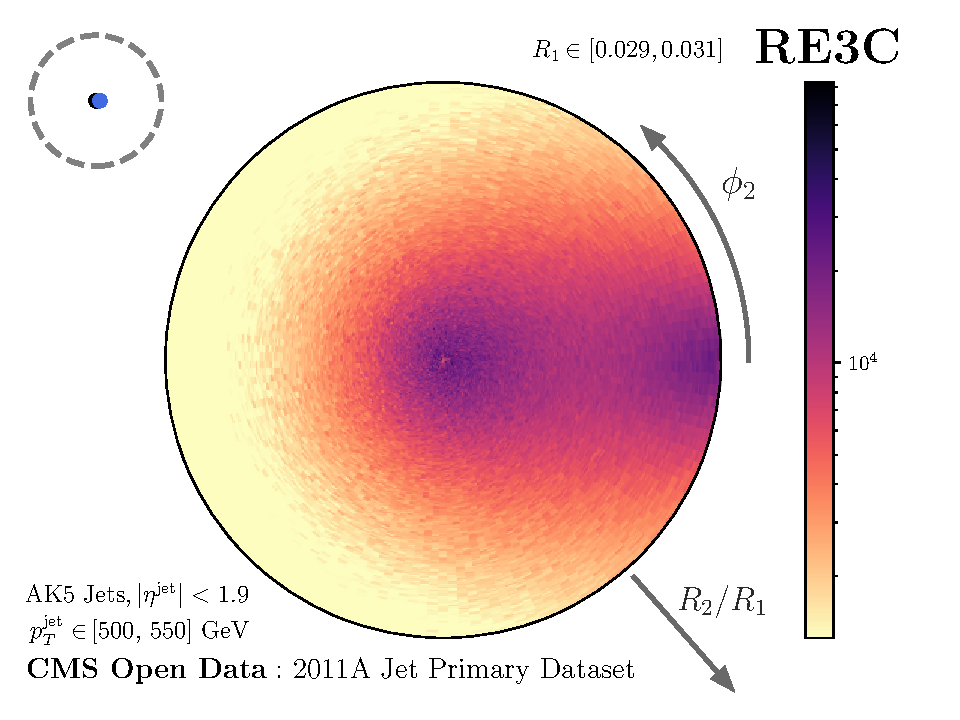
\includegraphics[width=0.32\textwidth]{figures/eec-angles/opendata/od_3particle_bullseye_0.0299352.pdf}
     }
    \subfloat[]{
    	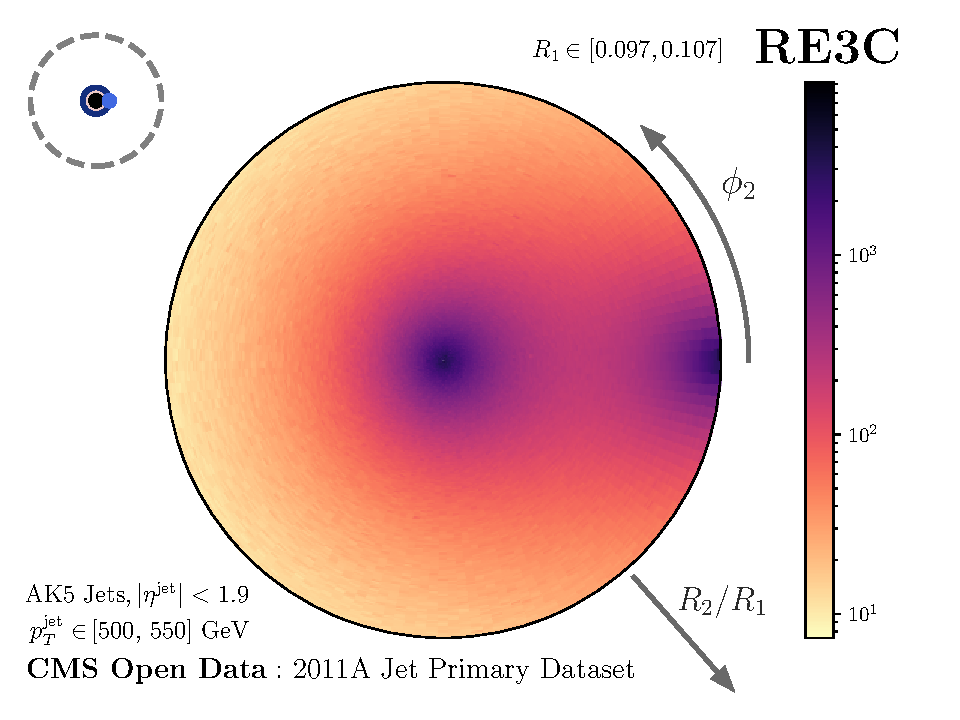
\includegraphics[width=0.32\textwidth]{figures/eec-angles/opendata/od_3particle_bullseye_0.101766.pdf}
     }
    \subfloat[]{
    	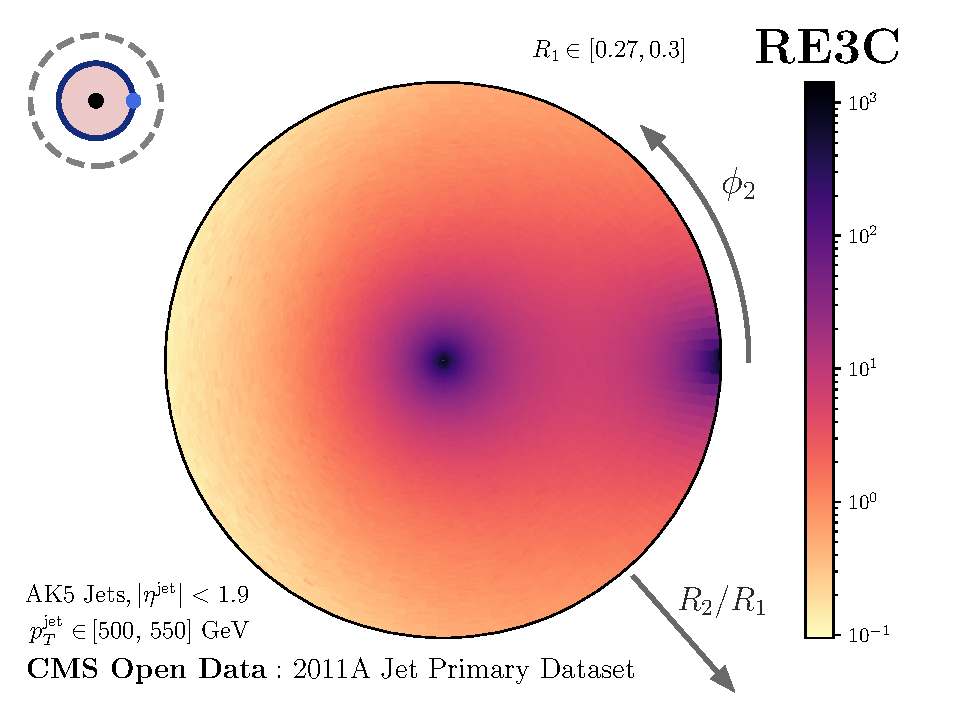
\includegraphics[width=0.32\textwidth]{figures/eec-angles/opendata/od_3particle_bullseye_0.286592.pdf}
     }
     \caption[Additional polar heat maps for RE3Cs evaluated on CMS Open Data.]
    {
        Additional polar heat maps for RE3Cs evaluated on CMS Open Data.
        %
        There are enhanced correlations when \(R_2\sim 0\), corresponding to the collinear enhancement
        as \(i_2\) approaches \(s\), and when \(\phi_2 \sim 0\), \(R_2 \sim R_1\), corresponding to \(i_2 \to\) \(i_1\).
        %
        The \(R_1\) bin for each plot is indicated by the radius of the filled circle in the top-left inset of each plot.
    }
    \label{fig:cms_re3cs}
\end{figure}
\begin{figure}[ht!]
    % \centering
    \subfloat[]{
    	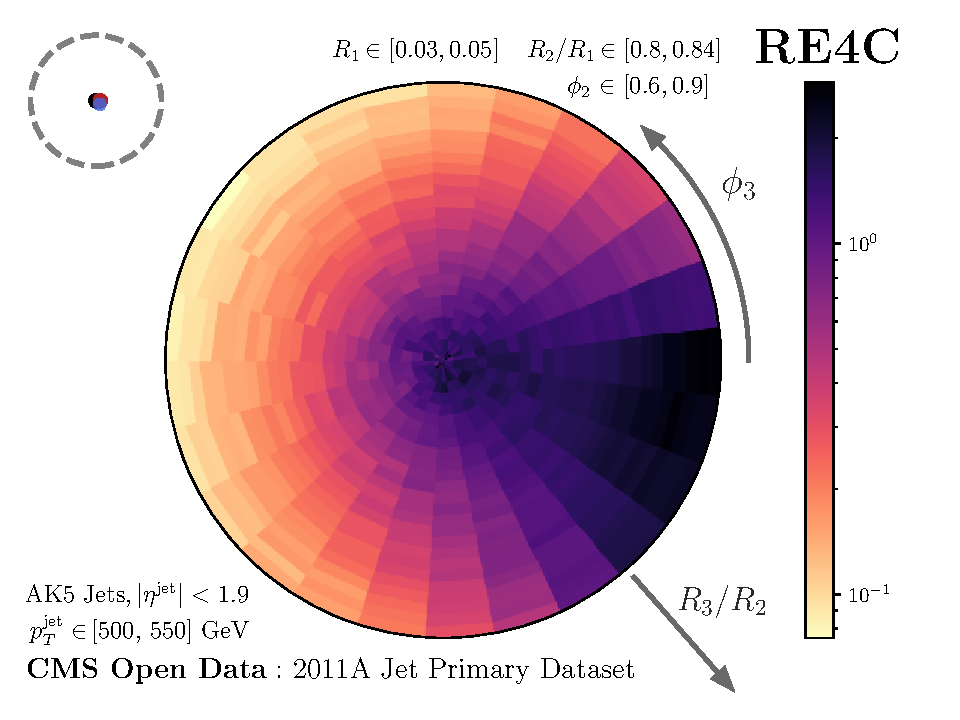
\includegraphics[width=0.32\textwidth]{figures/eec-angles/opendata/od_4particle_bullseye_0.0401108_0.82_0.753982.pdf}
    }
    \subfloat[]{
    	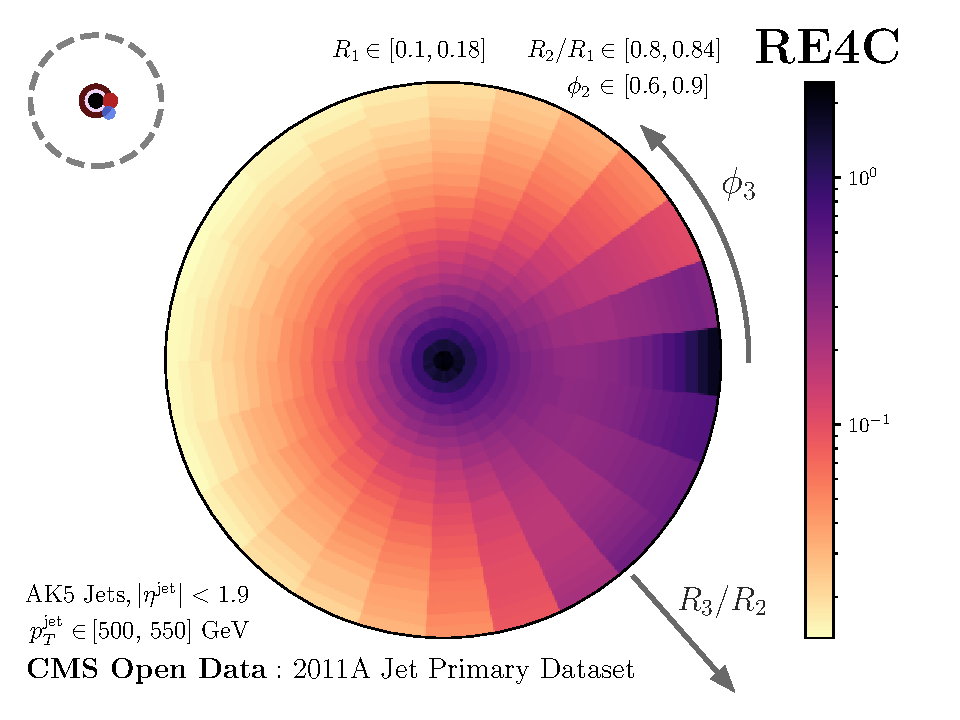
\includegraphics[width=0.32\textwidth]{figures/eec-angles/opendata/od_4particle_bullseye_0.134694_0.82_0.753982.pdf}
    }
    \subfloat[]{
    	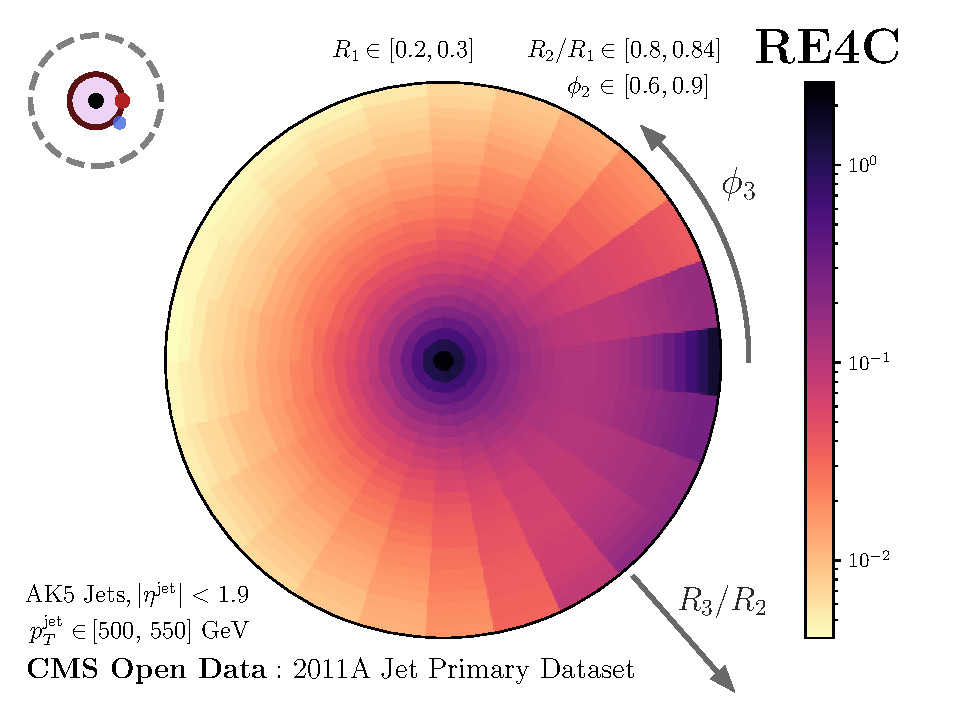
\includegraphics[width=0.32\textwidth]{figures/eec-angles/opendata/od_4particle_bullseye_0.246826_0.82_0.753982.pdf}
     }
    \\
    \vspace{-8pt}
     \subfloat[]{
    	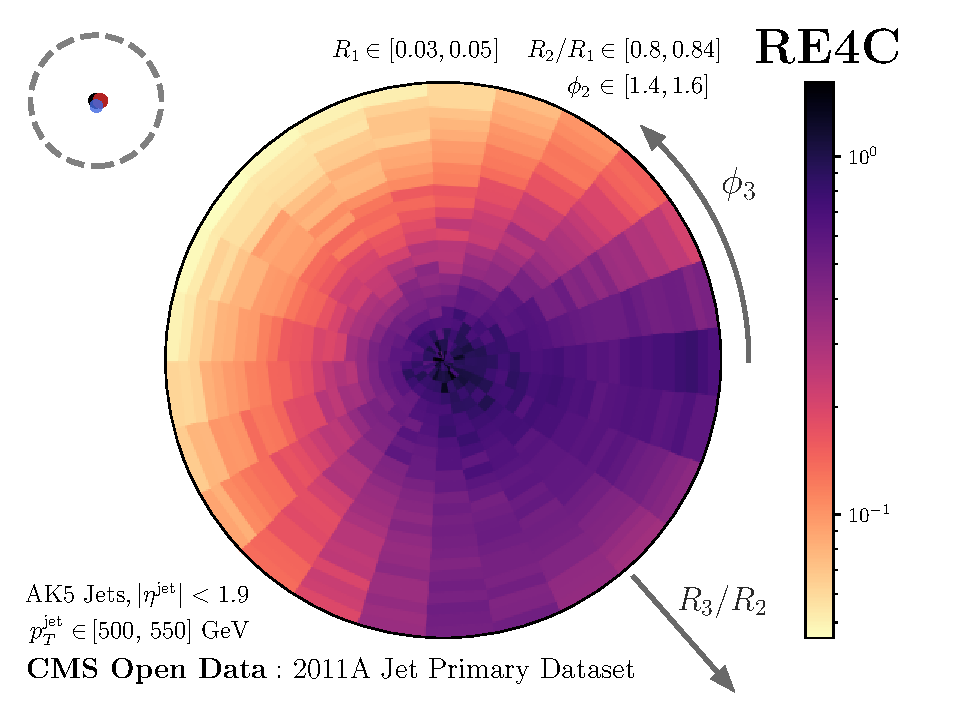
\includegraphics[width=0.32\textwidth]{figures/eec-angles/opendata/od_4particle_bullseye_0.0401108_0.82_1.50796.pdf}
    }
    \subfloat[]{
    	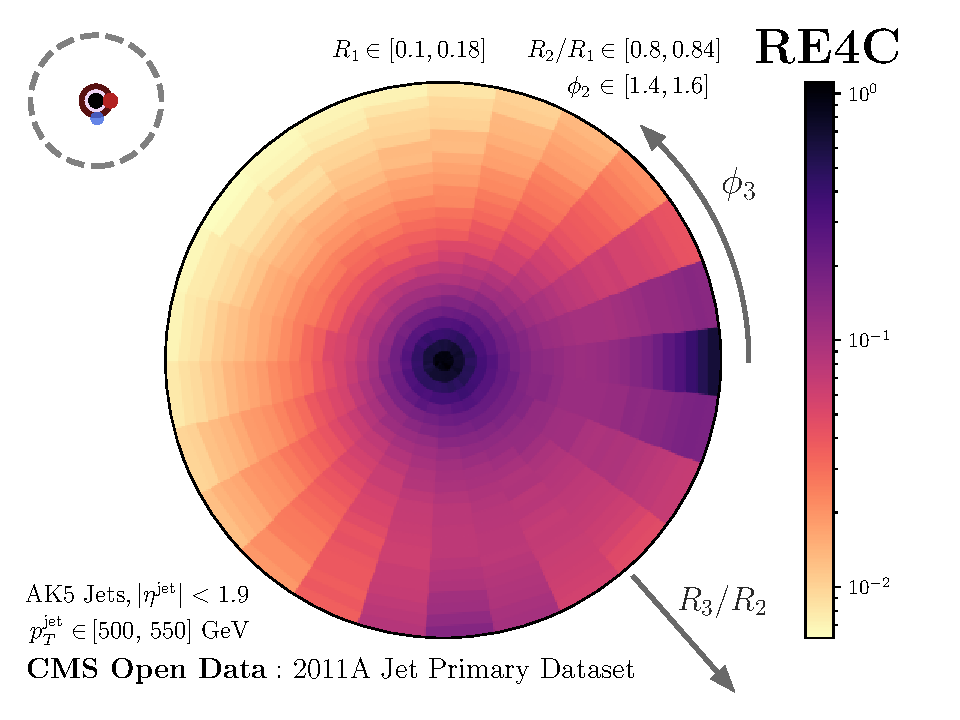
\includegraphics[width=0.32\textwidth]{figures/eec-angles/opendata/od_4particle_bullseye_0.134694_0.82_1.50796.pdf}
    }
    \subfloat[]{
    	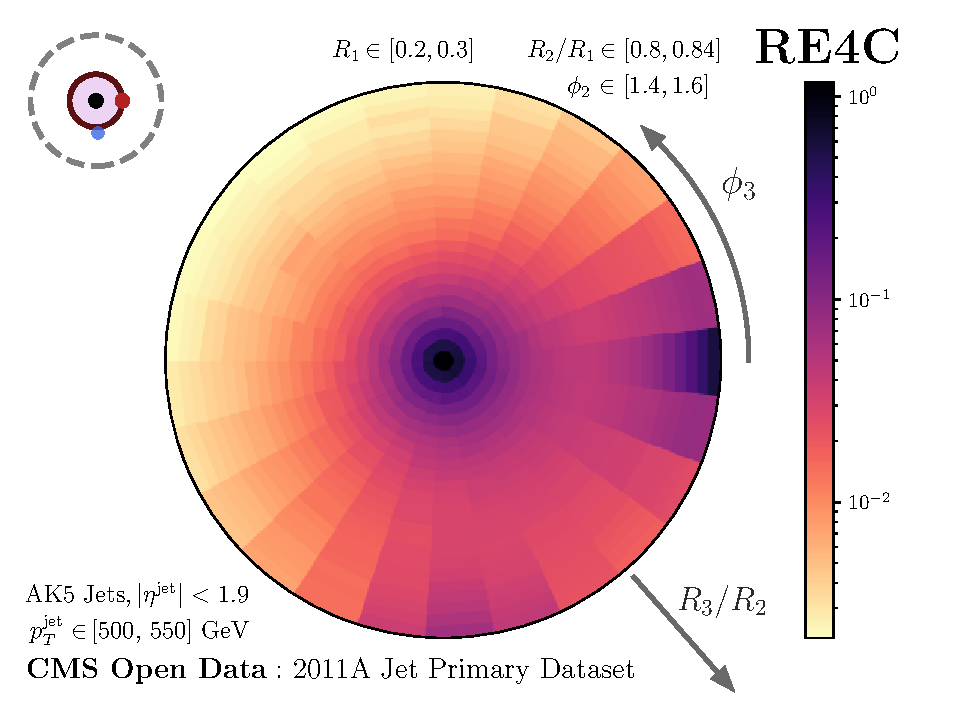
\includegraphics[width=0.32\textwidth]{figures/eec-angles/opendata/od_4particle_bullseye_0.246826_0.82_1.50796.pdf}
    }
    \\
    \vspace{-8pt}
     \subfloat[]{
    	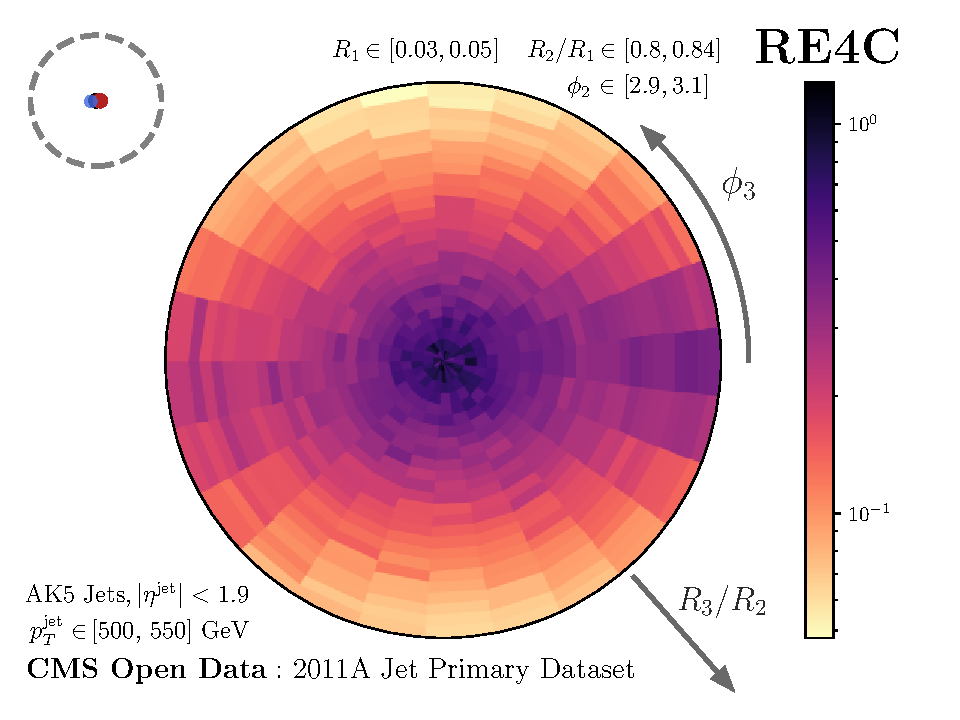
\includegraphics[width=0.32\textwidth]{figures/eec-angles/opendata/od_4particle_bullseye_0.0401108_0.82_3.01593.pdf}
    }
    \subfloat[]{
    	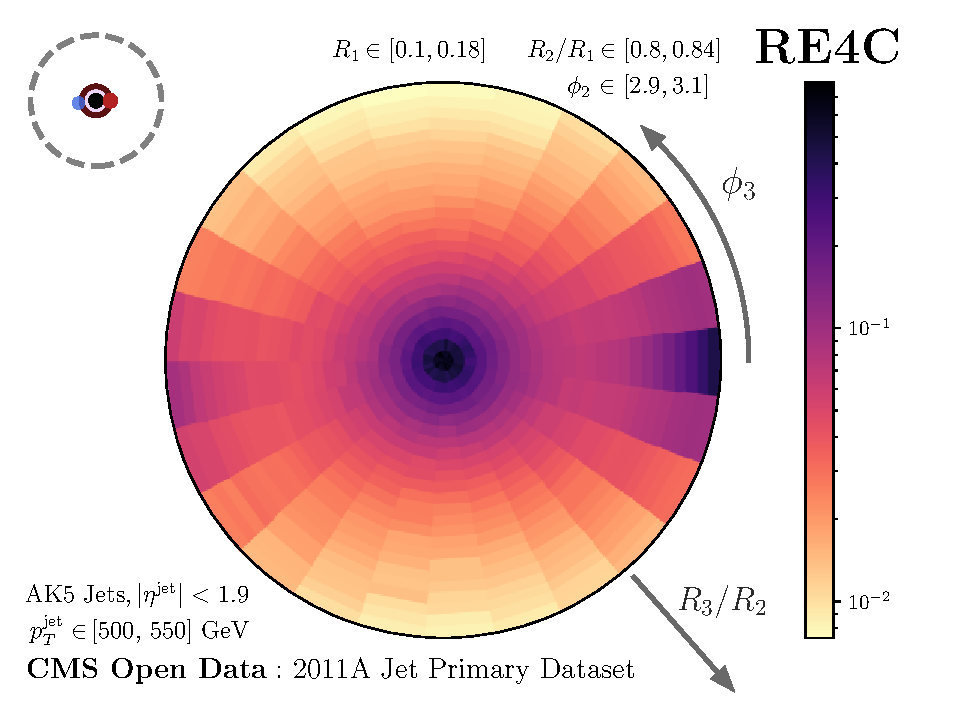
\includegraphics[width=0.32\textwidth]{figures/eec-angles/opendata/od_4particle_bullseye_0.134694_0.82_3.01593.pdf}
    }
    \subfloat[]{
    	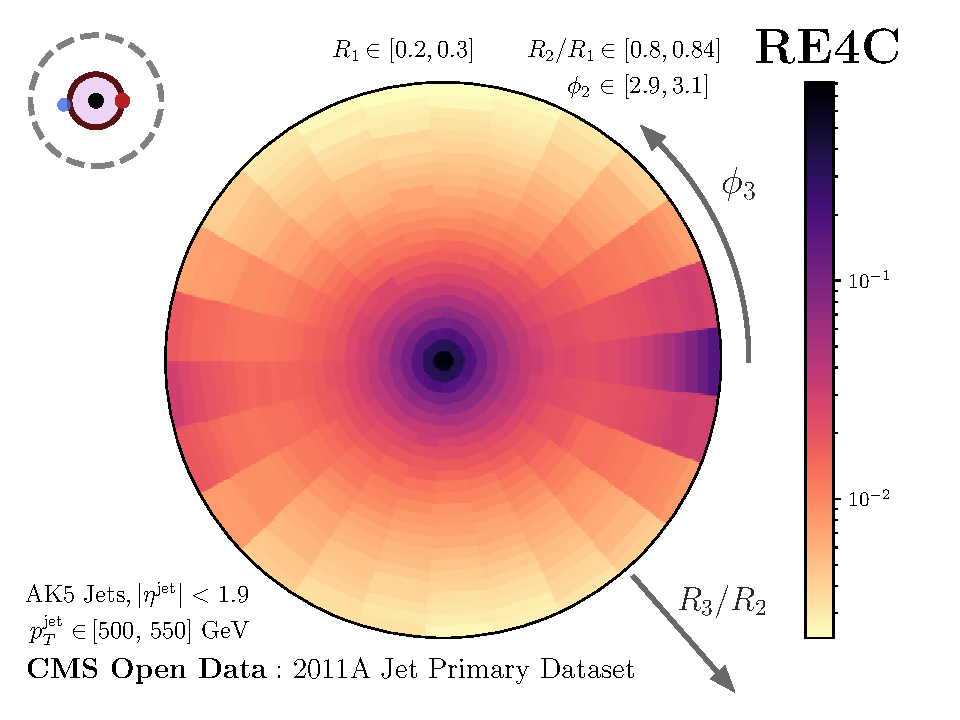
\includegraphics[width=0.32\textwidth]{figures/eec-angles/opendata/od_4particle_bullseye_0.246826_0.82_3.01593.pdf}
    }
    \caption[Polar heat maps for RE4Cs evaluated on CMS Open Data.]{
        Polar heat maps for RE4Cs evaluated on CMS Open Data, with \(\phi_2\) centered near $45^\circ$ (top row), $90^\circ$ (middle row) and $180^\circ$ (bottom row).
        %
        We highlight that, relative to the RE3C presented in \Fig{cms_re3cs}, there are enhanced correlations when \(\phi_3 \sim -\phi_2\), corresponding to the collinear enhancement of radiation as \(i_3\) approaches \(i_1\).
    }
    \label{fig:cms_re4cs}
\end{figure}



We now turn to our simulated samples of QCD, \(W\), and top jets.
%
We begin by showing \glspl{penc} evaluated on each jet sample in \Fig{pythia_pencs}, which provide simple, albeit less fetching, visualizations which clearly distinguish each sample of jets.
\begin{figure}[t]
    % \centering
    \subfloat[]{
    	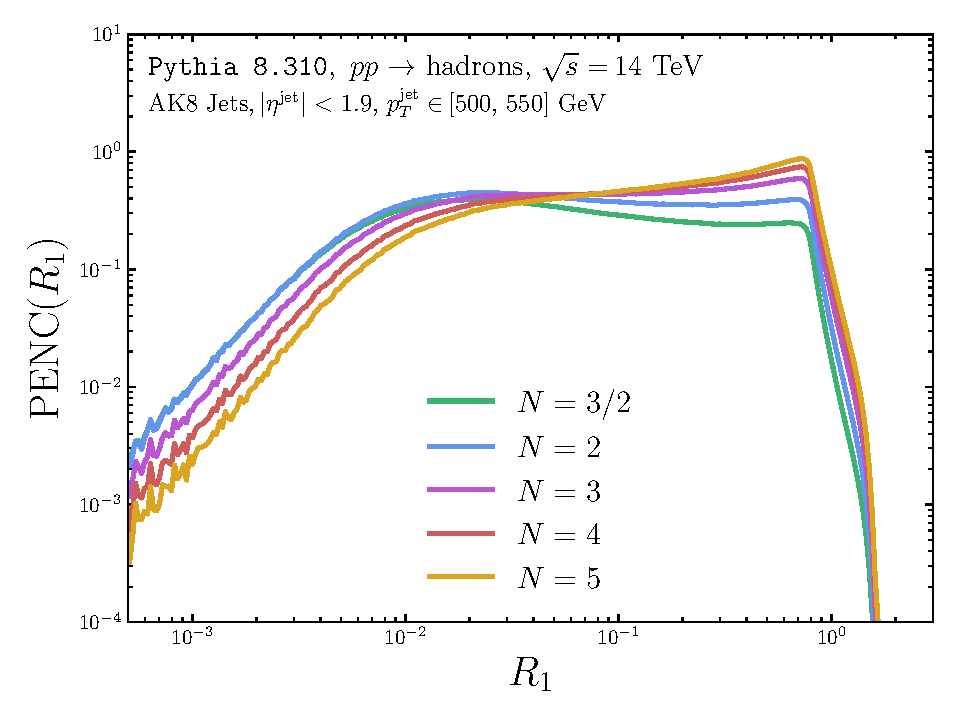
\includegraphics[width=0.34\textwidth]{figures/eec-angles/supplemental/2particle/qcd_combined_1d.pdf}
    }
    \subfloat[]{
    	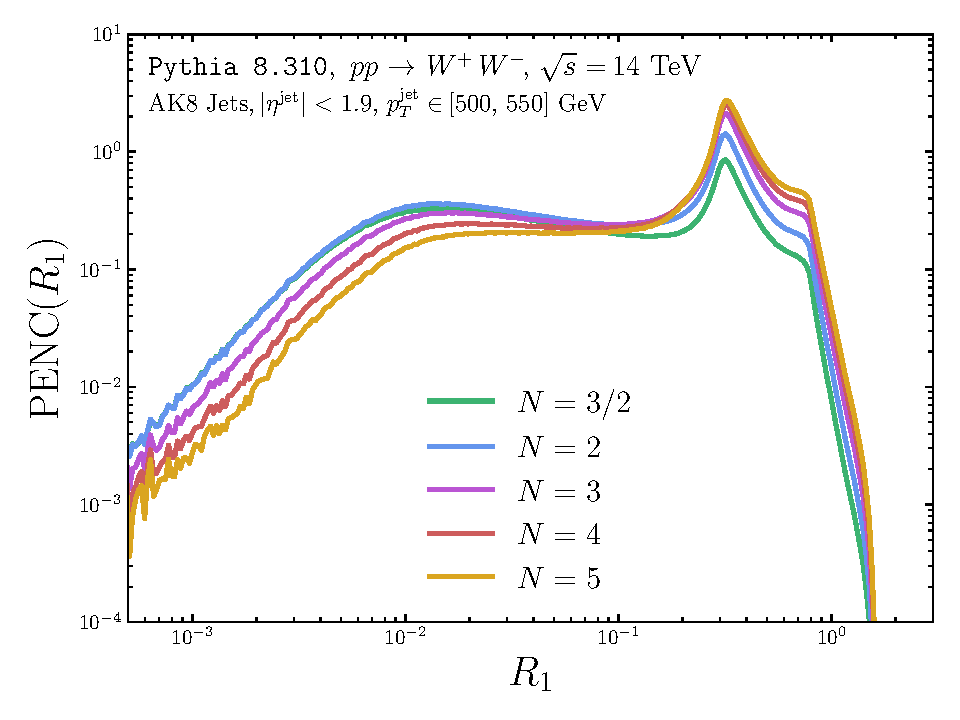
\includegraphics[width=0.34\textwidth]{figures/eec-angles/supplemental/2particle/w_combined_1d.pdf}
    }
    \subfloat[]{
    	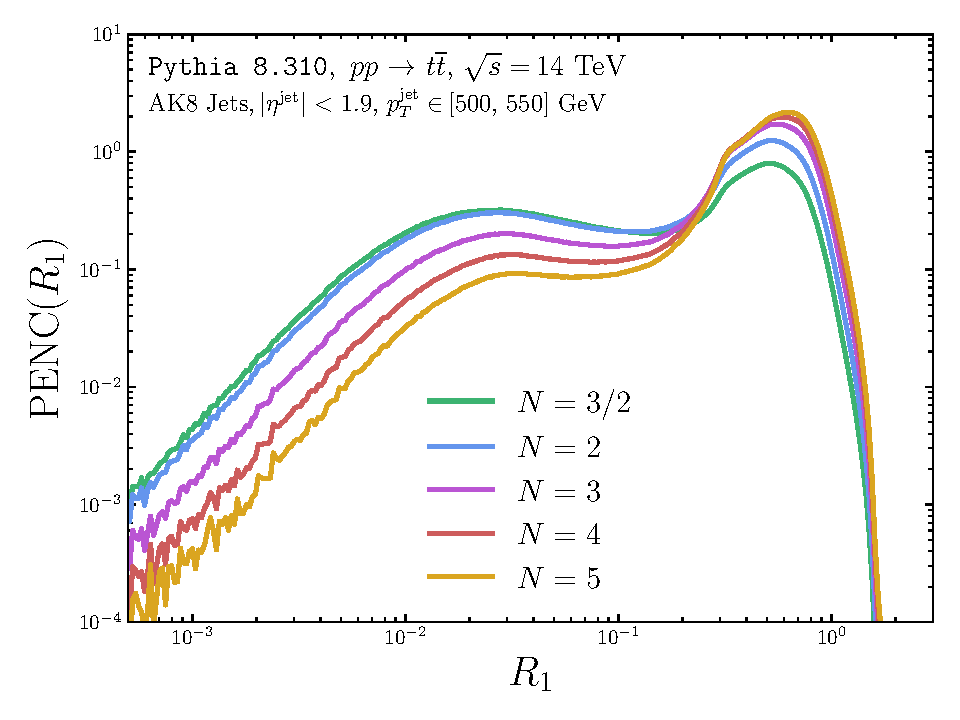
\includegraphics[width=0.34\textwidth]{figures/eec-angles/supplemental/2particle/top_combined_1d.pdf}
    }
    \caption[Projected energy correlators on simulated QCD, \(W\), and top jets.]{
        \glspl{penc} for {\textbf{(a)}} QCD-, {\textbf{(b)}} $W$- and {\textbf{(c)}} top-quark-initiated jet samples generated with \texttt{Pythia 8.310}.
        %
        Jets are clustered using the anti-$k_t$ algorithm with a radius parameter of $R=0.8$, and have transverse momenta in the range $p_T^{\rm jet} \in [500,550] \,\text{GeV}$ and psuedo-rapidities in the range $\vert \eta^{\rm jet}\vert < 1.9$.
        %
        \glspl{penc} for $W$- and top-quark-initiated jets feature enhanced correlations at scales correlated with the $W$-boson and top-quark masses.
    }
	\label{fig:pythia_pencs}%
\end{figure}

The visually distinct features of each jet sample are even more evident as more particles are resolved, i.e.~by the RE3C and RE4C.
%
In \Fig{pythia_re3cs}, we present bullseye visualizations of the RE3C for each jet sample in several \(R_1\) bins;
%
as in the plots using CMS Open Data in the previous appendix, the radial variable and polar angle for each RE3C bullseye are the ratio \(R_2/R_1\) and the angle \(\phi_2\), respectively.
%
We note that the rings in the polar heat maps for the RE3C are correlated with the mass of the \(W\) boson, in that they appear at the angular scale \(R_2 \simeq 0.3 \sim 2 m_W / p_T^\text{jet}\).

The bullseye of representation of the RE3C we introduce are similar to the analogous bullseye representations of the traditional E3C for each jet sample, shown in \Fig{pythia_old_e3cs}, for which the radial variable is the ratio \(R_S/R_L\) and the polar angle is the associated azimuthal angle.
%
However, the traditional E3C shows only a small slice of the information of the RE3C we introduce in this work, and the RE3C introduced in this work contains additional information about the relative orientations of particles within a jet;
%
for example, \Figs{w_medium_re3c}{w_large_re3c} can be compared to \Figs{w_medium_trade3c}{w_large_trade3c} to conclude that the RE3C we introduce conveys additional information about the orientation of the rings of radiation within \(W\)-boson-initiated jets.

\begin{figure}
    \centering
    \subfloat[]{
    	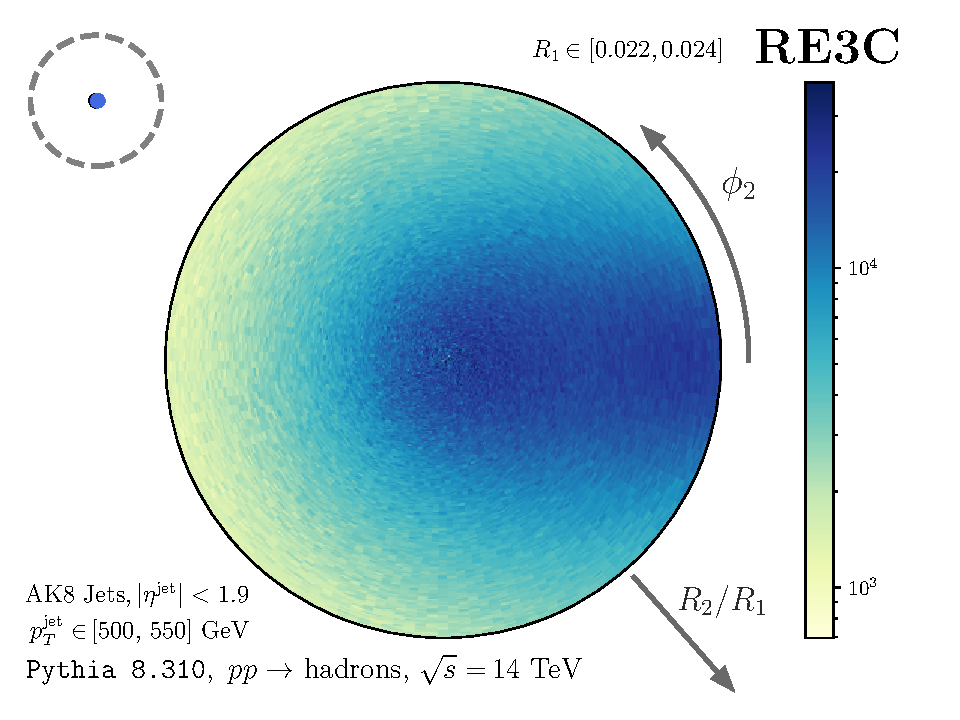
\includegraphics[width=0.34\textwidth]{figures/eec-angles/supplemental/3particle/qcd0.0225708_3particle_bullseye.pdf}
    }
    \subfloat[]{
    	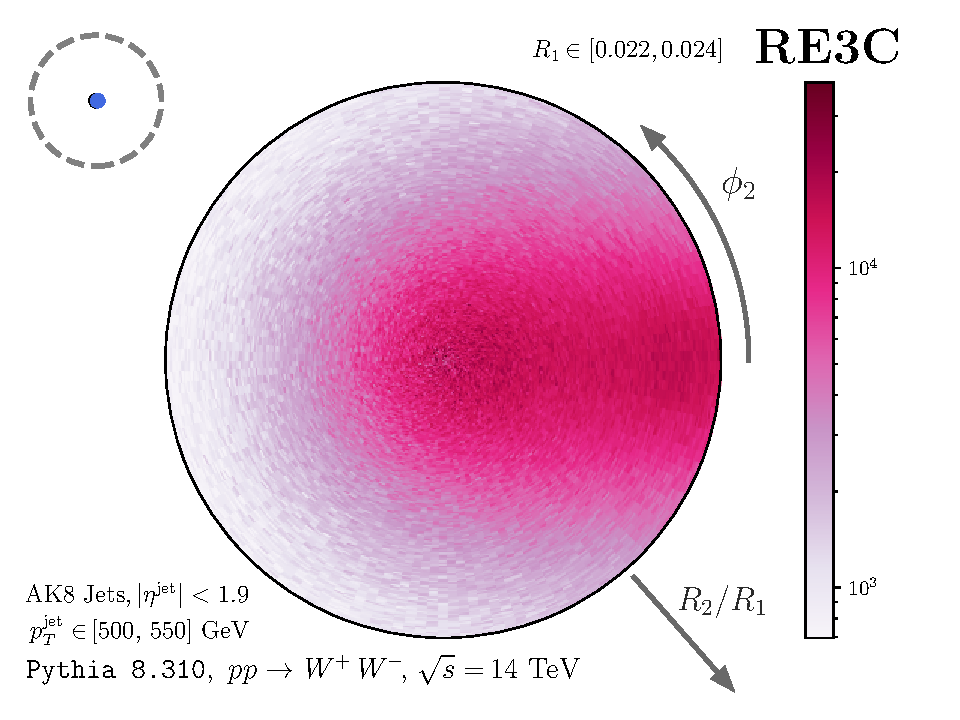
\includegraphics[width=0.34\textwidth]{figures/eec-angles/supplemental/3particle/w0.0225708_3particle_bullseye.pdf}
    }
    \subfloat[]{
    	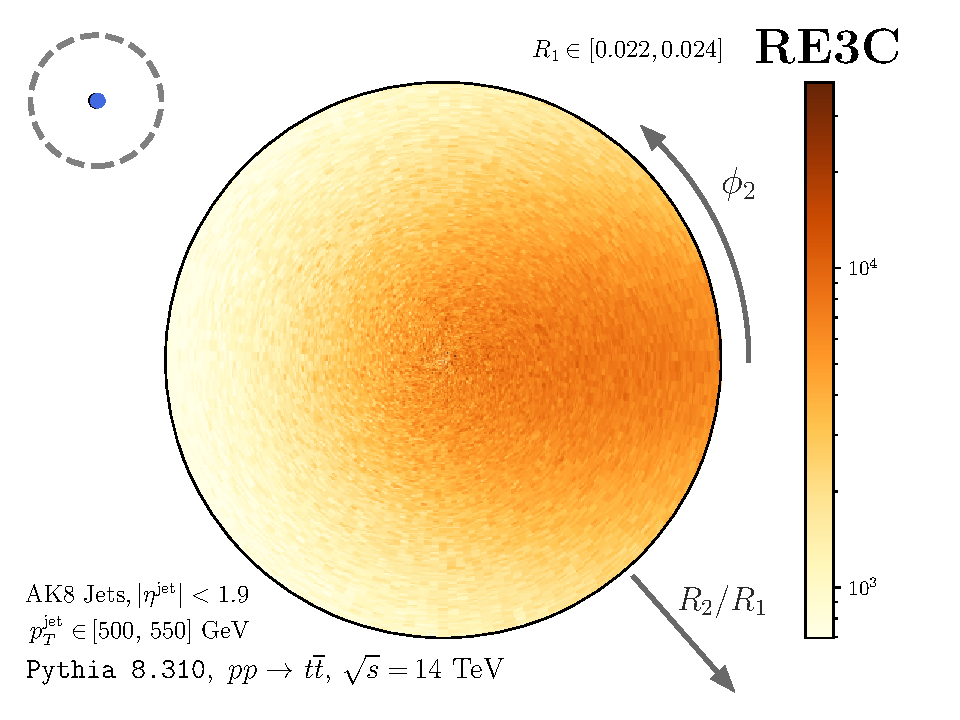
\includegraphics[width=0.34\textwidth]{figures/eec-angles/supplemental/3particle/top0.0225708_3particle_bullseye.pdf}
    }
    \\
    \subfloat[]{
    	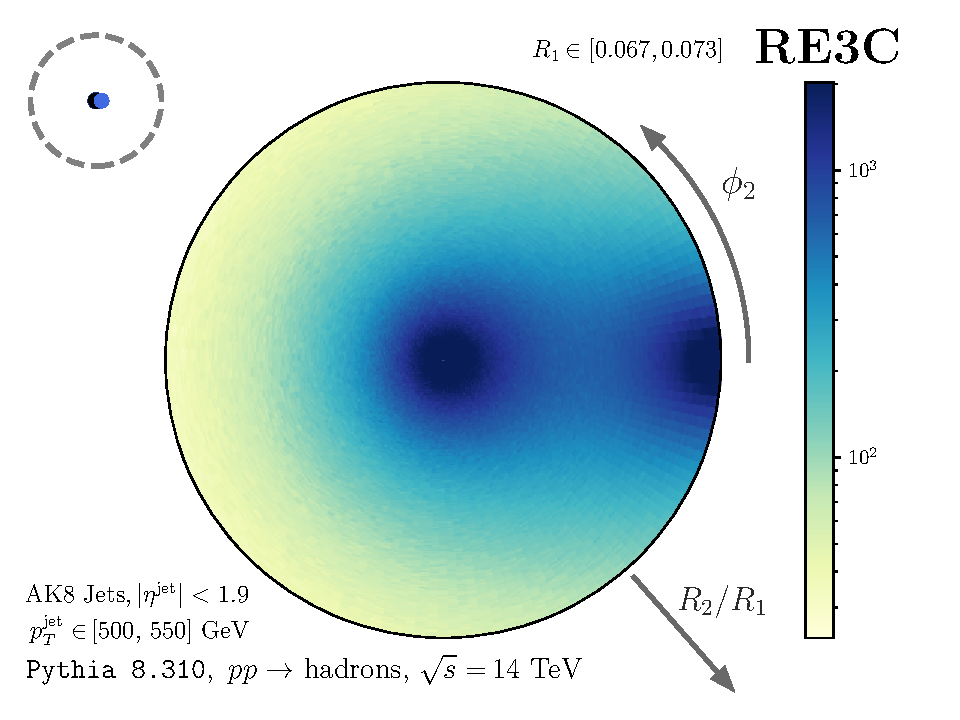
\includegraphics[width=0.34\textwidth]{figures/eec-angles/supplemental/3particle/qcd0.0698374_3particle_bullseye.pdf}
    }
    \subfloat[]{
    	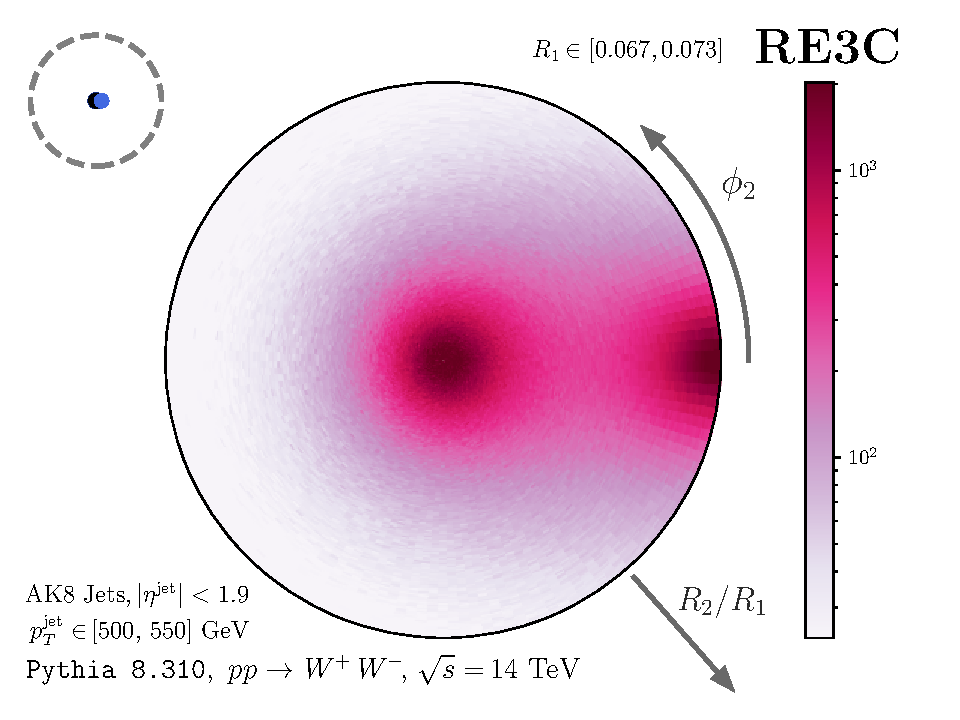
\includegraphics[width=0.34\textwidth]{figures/eec-angles/supplemental/3particle/w0.0698374_3particle_bullseye.pdf}
    }
    \subfloat[]{
    	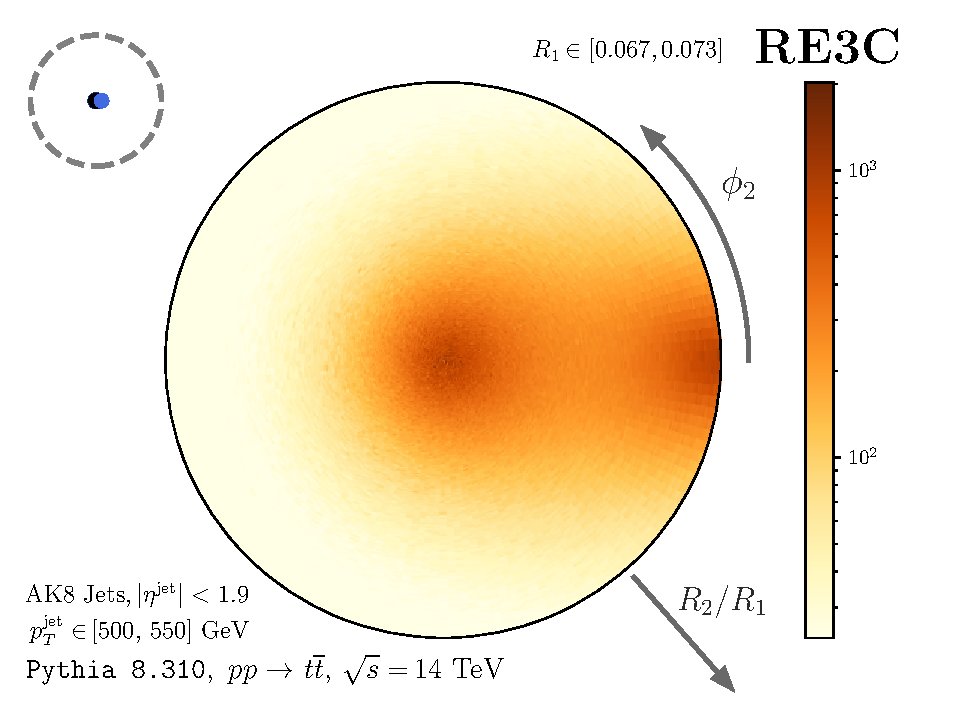
\includegraphics[width=0.34\textwidth]{figures/eec-angles/supplemental/3particle/top0.0698374_3particle_bullseye.pdf}
    }
    \\
    \subfloat[]{
    	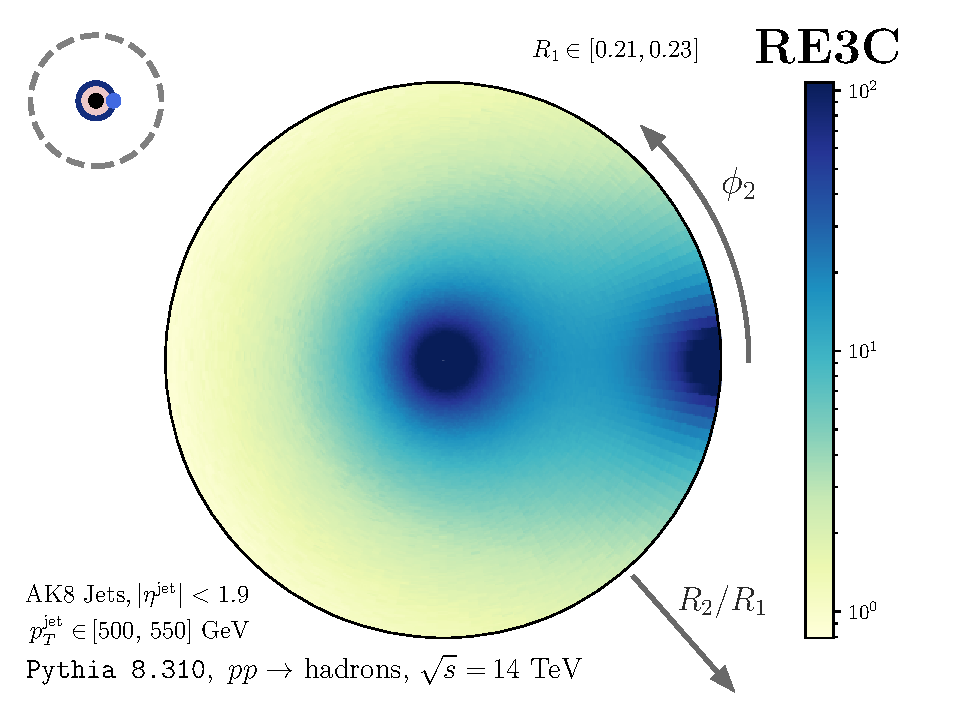
\includegraphics[width=0.34\textwidth]{figures/eec-angles/supplemental/3particle/qcd0.216087_3particle_bullseye.pdf}
    }
    \subfloat[]{
    	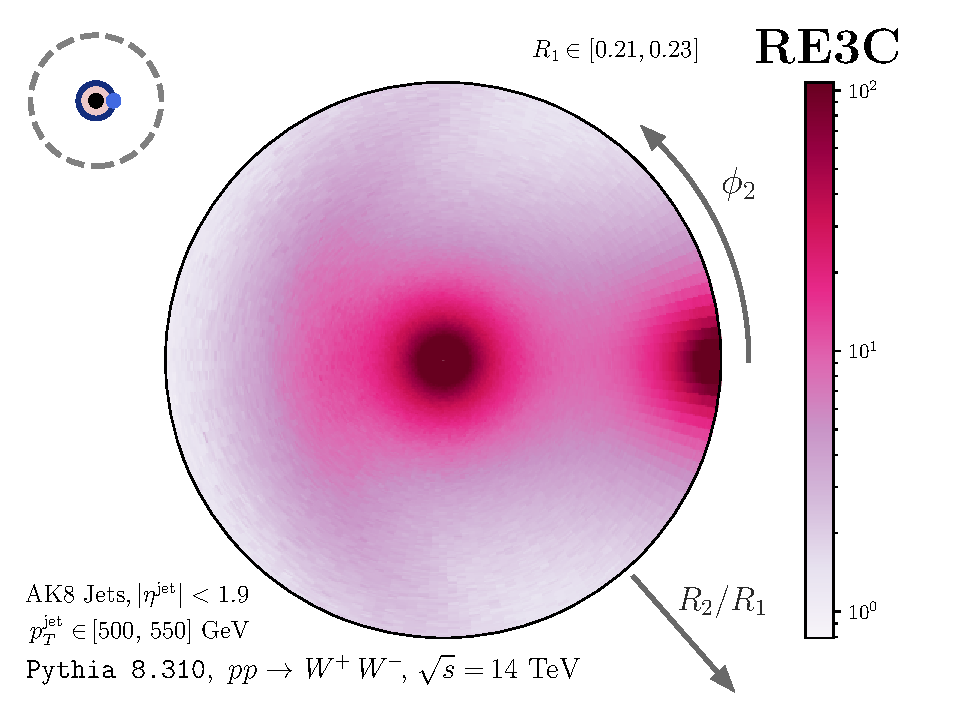
\includegraphics[width=0.34\textwidth]{figures/eec-angles/supplemental/3particle/w0.216087_3particle_bullseye.pdf}
        \label{fig:w_medium_re3c}
    }
    \subfloat[]{
    	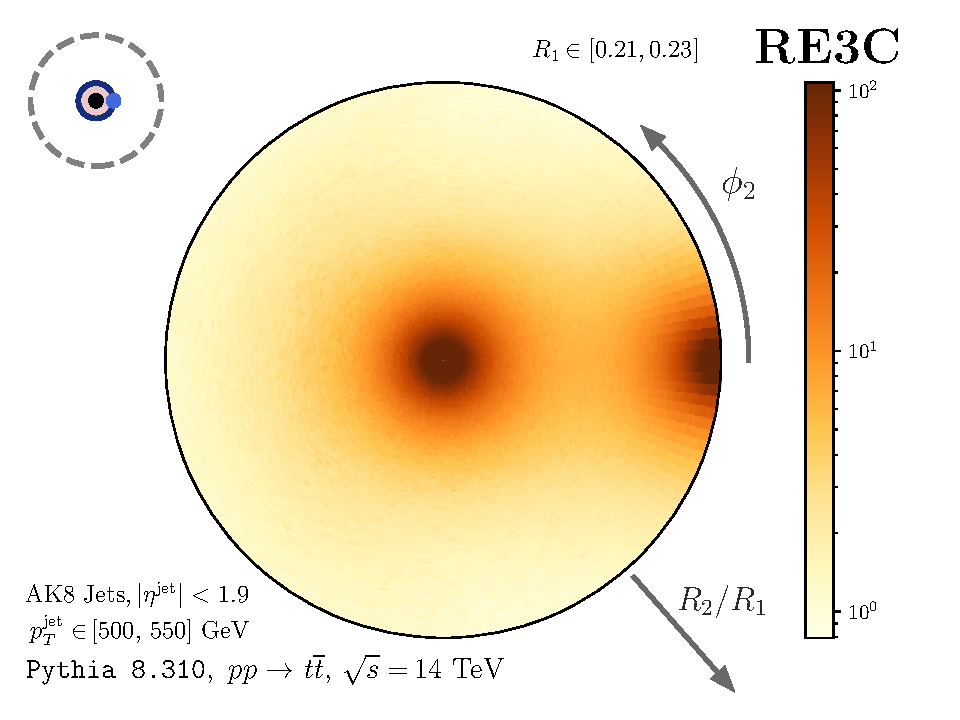
\includegraphics[width=0.34\textwidth]{figures/eec-angles/supplemental/3particle/top0.216087_3particle_bullseye.pdf}
    }
    \\
    \subfloat[]{
    	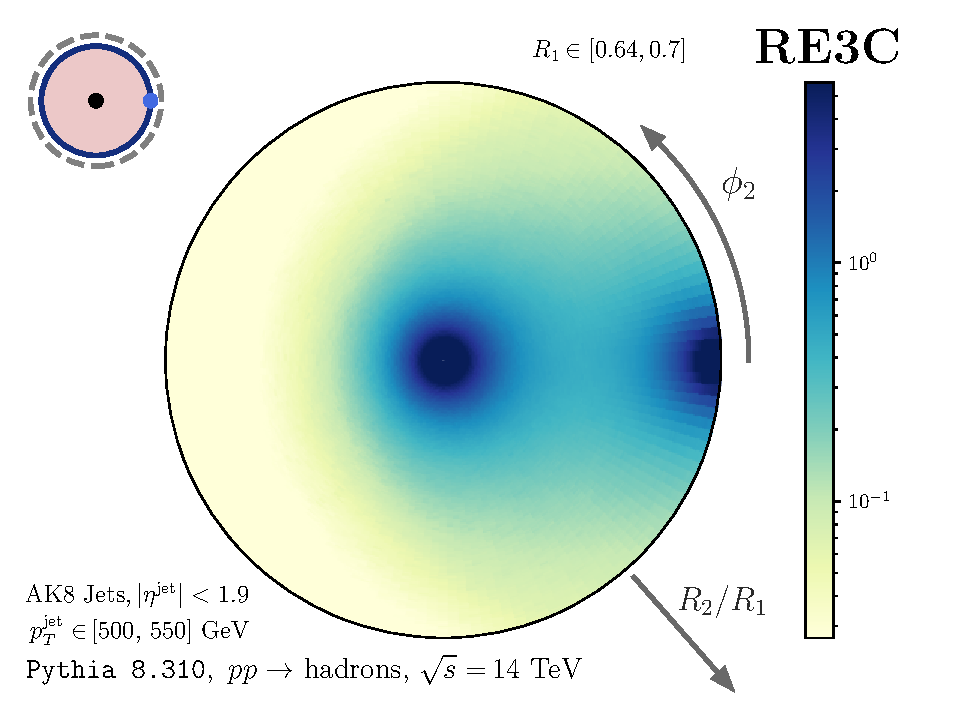
\includegraphics[width=0.34\textwidth]{figures/eec-angles/supplemental/3particle/qcd0.668604_3particle_bullseye.pdf}
    }
    \subfloat[]{
    	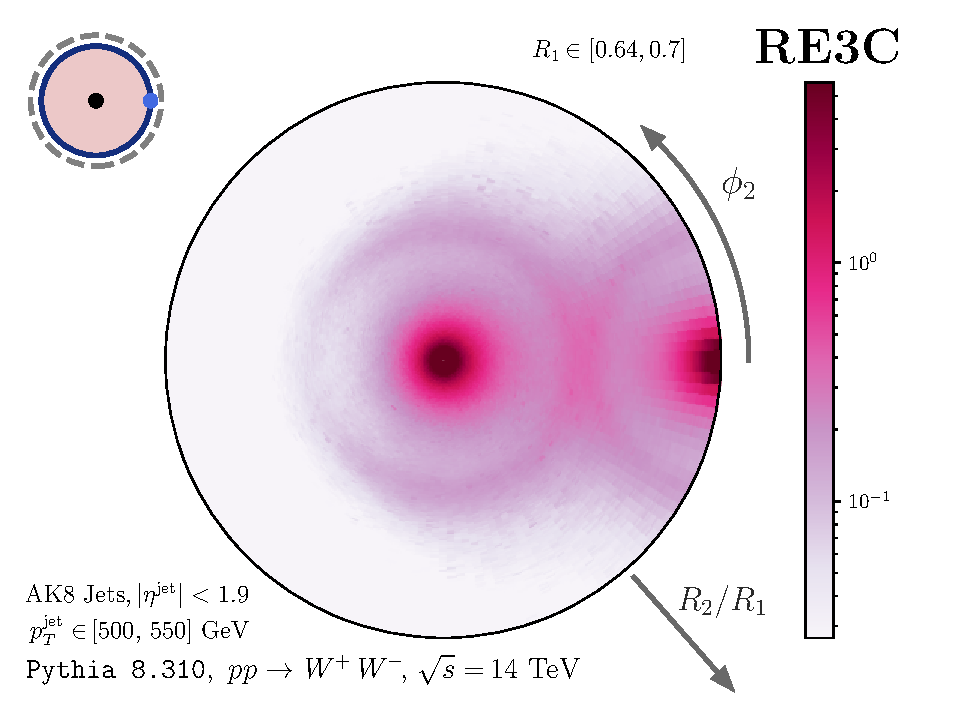
\includegraphics[width=0.34\textwidth]{figures/eec-angles/supplemental/3particle/w0.668604_3particle_bullseye.pdf}
        \label{fig:w_large_re3c}
    }
    \subfloat[]{
    	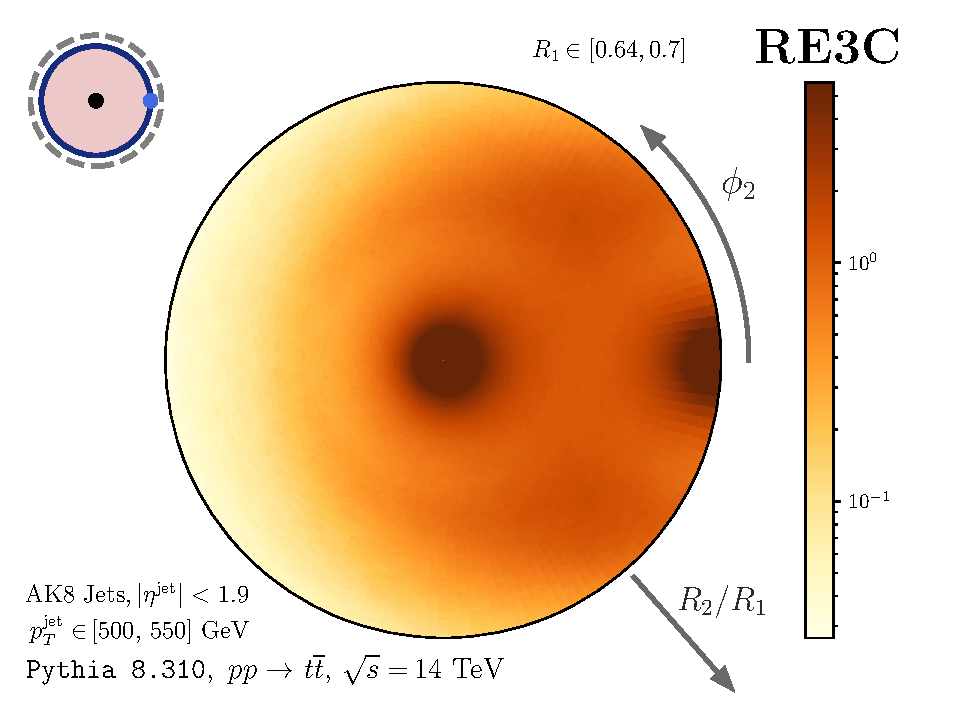
\includegraphics[width=0.34\textwidth]{figures/eec-angles/supplemental/3particle/top0.668604_3particle_bullseye.pdf}
    }
    \caption[Polar heat maps of the resolved three-point energy corrleator on QCD, \(W\), and top jets.]{
        Polar heat maps of the RE3C we introduce in this work for (first column) QCD-, (second column) \(W\)-, and (third column) top-quark-initiated jets.
        %
        The radial direction in each plot is the ratio \(R_1/R_2\), and the polar angle of each plot indicates the angle \(\phi_2\).
        %
        Our RE3Cs provide a clear visual representation of the distinct patterns of radiation in each jet sample at different scales (set by \(R_1\)).
    }
	\label{fig:pythia_re3cs}%
\end{figure}

\begin{figure}
    \centering
    \subfloat[]{
    	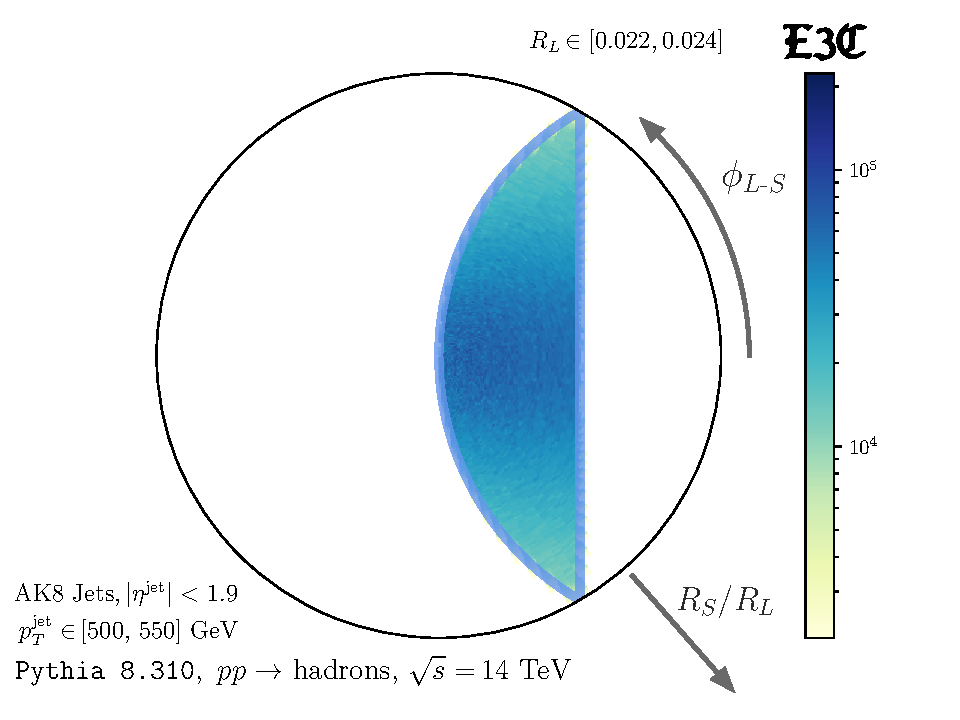
\includegraphics[width=0.34\textwidth]{figures/eec-angles/supplemental/wedge/qcd0.0225708_3particle_bullseye.pdf}
    }
    \subfloat[]{
    	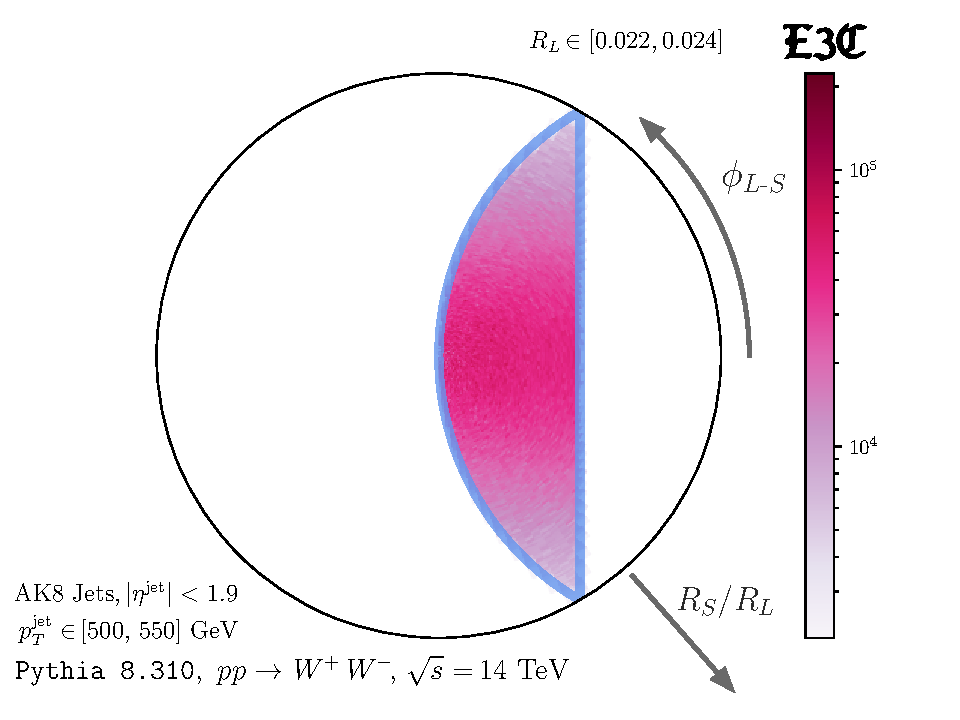
\includegraphics[width=0.34\textwidth]{figures/eec-angles/supplemental/wedge/w0.0225708_3particle_bullseye.pdf}
    }
    \subfloat[]{
    	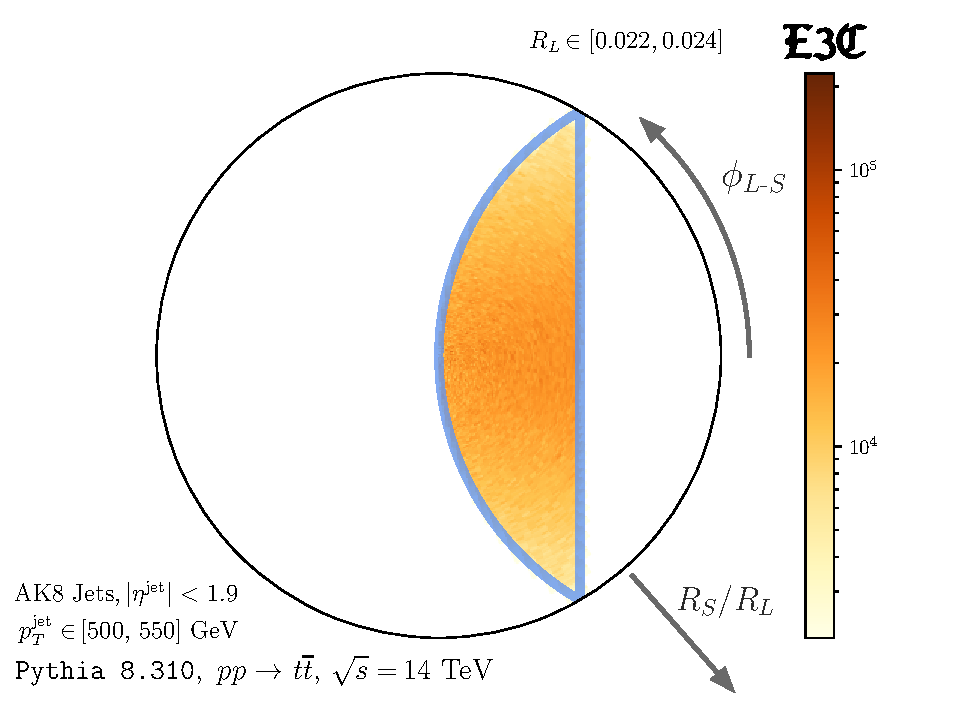
\includegraphics[width=0.34\textwidth]{figures/eec-angles/supplemental/wedge/top0.0225708_3particle_bullseye.pdf}
    }
    \\
    \subfloat[]{
    	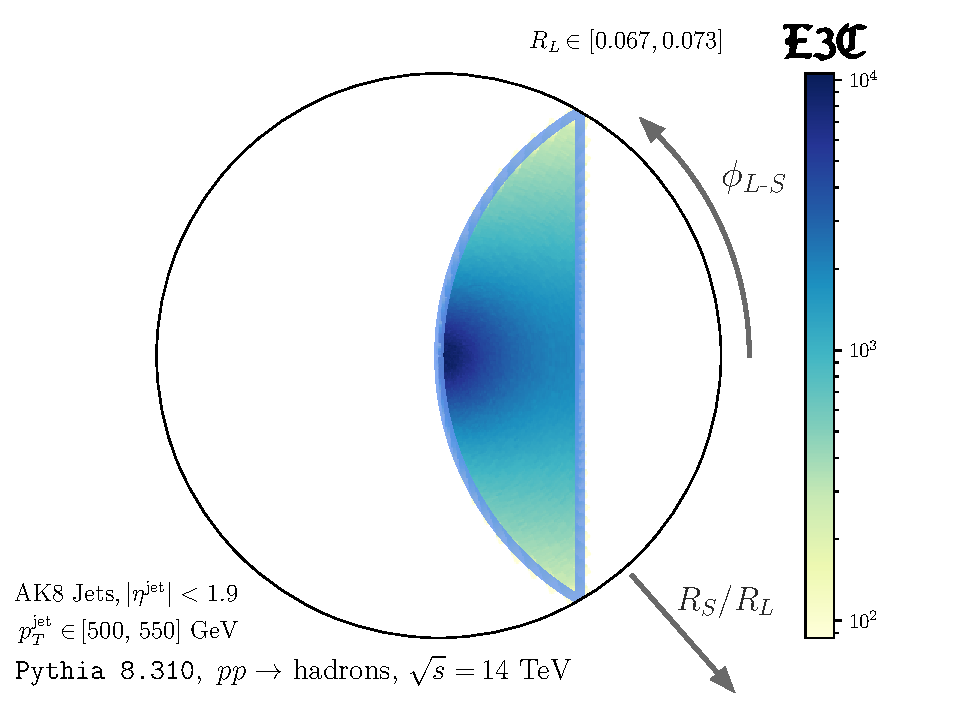
\includegraphics[width=0.34\textwidth]{figures/eec-angles/supplemental/wedge/qcd0.0698374_3particle_bullseye.pdf}
    }
    \subfloat[]{
    	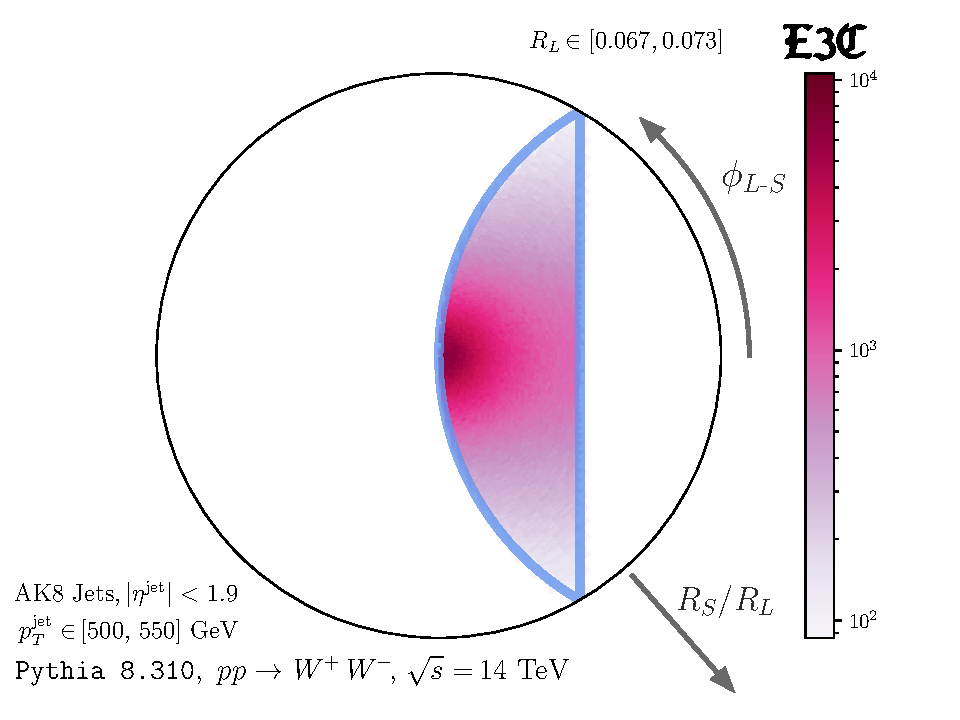
\includegraphics[width=0.34\textwidth]{figures/eec-angles/supplemental/wedge/w0.0698374_3particle_bullseye.pdf}
    }
    \subfloat[]{
    	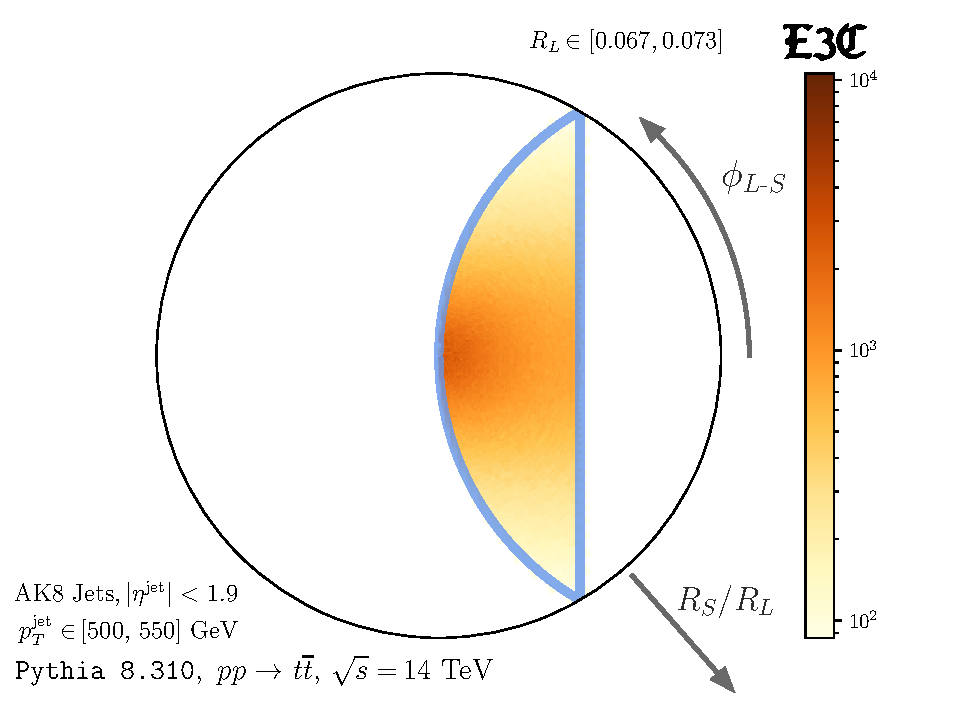
\includegraphics[width=0.34\textwidth]{figures/eec-angles/supplemental/wedge/top0.0698374_3particle_bullseye.pdf}
    }
    \\
    \subfloat[]{
    	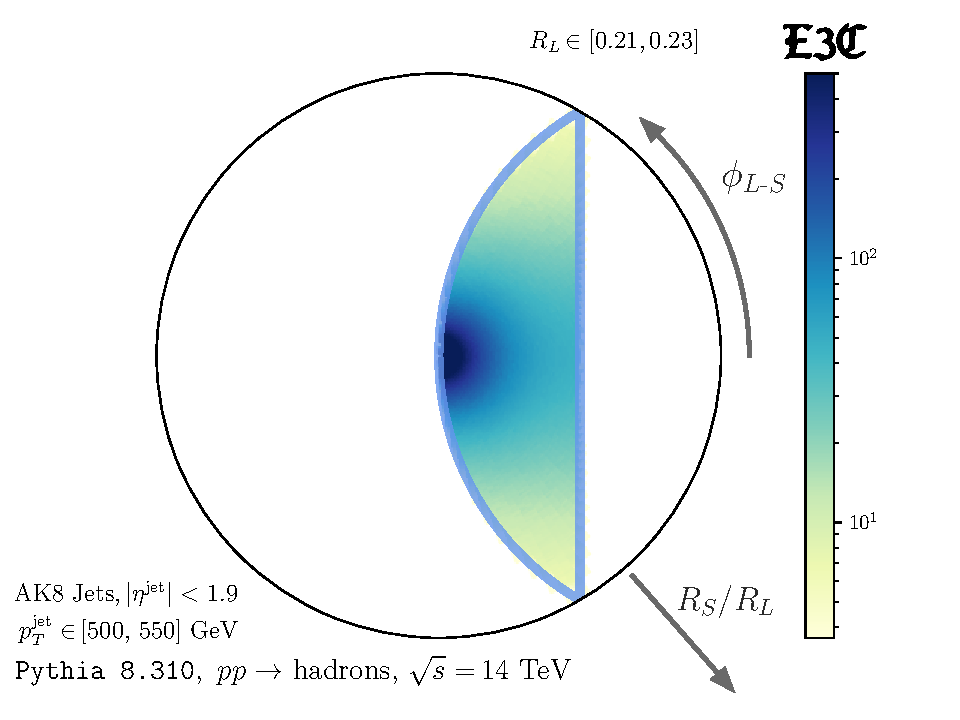
\includegraphics[width=0.34\textwidth]{figures/eec-angles/supplemental/wedge/qcd0.216087_3particle_bullseye.pdf}
    }
    \subfloat[]{
    	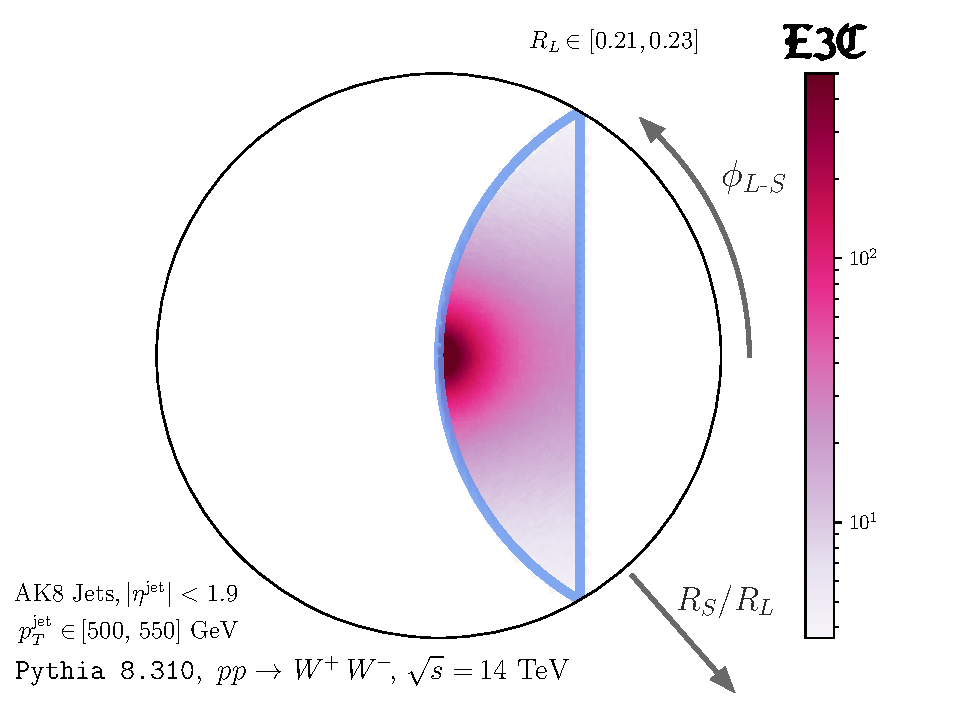
\includegraphics[width=0.34\textwidth]{figures/eec-angles/supplemental/wedge/w0.216087_3particle_bullseye.pdf}
        \label{fig:w_medium_trade3c}
    }
    \subfloat[]{
    	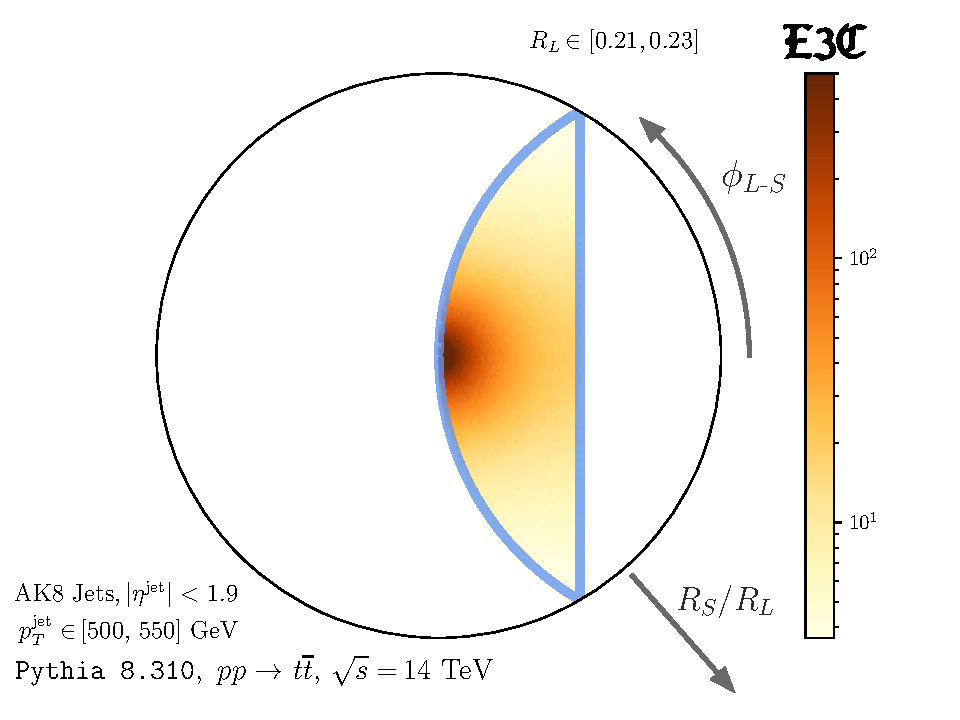
\includegraphics[width=0.34\textwidth]{figures/eec-angles/supplemental/wedge/top0.216087_3particle_bullseye.pdf}
    }
    \\
    \subfloat[]{
    	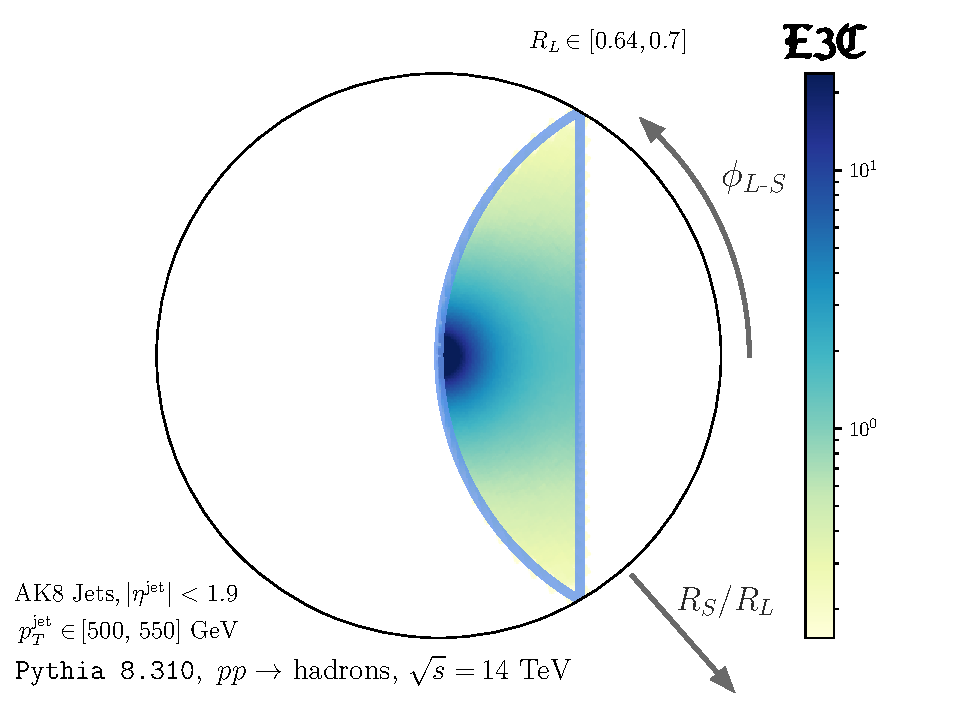
\includegraphics[width=0.34\textwidth]{figures/eec-angles/supplemental/wedge/qcd0.668604_3particle_bullseye.pdf}
    }
    \subfloat[]{
    	\includegraphics[width=0.34\textwidth]{figures/eec-angles/supplemental/wedge/w0.668604_3particle_bullseye.pdf}
        \label{fig:w_large_trade3c}
    }
    \subfloat[]{
    	\includegraphics[width=0.34\textwidth]{figures/eec-angles/supplemental/wedge/top0.668604_3particle_bullseye.pdf}
    }
    \caption[Polar heat maps of the traditional three-point energy correlator on QCD, \(W\), and top jets.]{
        Polar heat maps of the traditional E3C for (first column) QCD-, (second column) \(W\)-, and (third column) top-quark-initiated jets.
        %
        The radial direction in each plot is the ratio \(R_S/R_L\), and the polar angle of the plot corresponds to the angle between the lines whose lengths determine \(R_S\) and \(R_L\).
        %
        The \(R_L\) bins for each plot are chosen to be the same as the \(R_1\) bins in \Fig{pythia_re3cs}.
        %
        The polar heat maps of the traditional E3C contain similar information as the RE3Cs introduced in this work and shown in \Fig{pythia_re3cs};
        %
        however, the traditional E3C does not capture all the orientation information about radiation patterns in each jet sample that is present in our new RE3C.
    }
	\label{fig:pythia_old_e3cs}%
\end{figure}

\Fig{pythia_re4cs} provides similar polar heat maps for \(R_3/R_2\) and \(\phi_3\) for the RE4C, within several \(\phi_2\) bins, and for \(R_2\) near \(R_1\).
%
As in the case of the RE4Cs evaluated on CMS Open Data, we also see prominent correlations when \(\phi_3 \sim -\phi_2\) when \(R_2\) is near \(R_1\), corresponding to the case that particle \(i_3\) approaches particle \(i_1\).
%
These correlations for \(\phi_3 \sim -\phi_2\) quickly diminish as \(R_2\) is decreased and no longer near \(R_1\).

\begin{figure}[t]
    \centering
    \subfloat[]{
    	\includegraphics[width=0.34\textwidth]{figures/eec-angles/supplemental/4particle/qcd0.452309_0.82_0.753982_4particle_bullseye.pdf}
    }
    \subfloat[]{
    	\includegraphics[width=0.34\textwidth]{figures/eec-angles/supplemental/4particle/w0.452309_0.82_0.753982_4particle_bullseye.pdf}
    }
    \subfloat[]{
    	\includegraphics[width=0.34\textwidth]{figures/eec-angles/supplemental/4particle/top0.452309_0.82_0.753982_4particle_bullseye.pdf}
    }
    \\
    \vspace{-8pt}
    \subfloat[]{
    	\includegraphics[width=0.34\textwidth]{figures/eec-angles/supplemental/4particle/qcd0.452309_0.82_1.50796_4particle_bullseye.pdf}
    }
    \subfloat[]{
    	\includegraphics[width=0.34\textwidth]{figures/eec-angles/supplemental/4particle/w0.452309_0.82_1.50796_4particle_bullseye.pdf}
    }
    \subfloat[]{
    	\includegraphics[width=0.34\textwidth]{figures/eec-angles/supplemental/4particle/top0.452309_0.82_1.50796_4particle_bullseye.pdf}
    }
    \\
    \vspace{-8pt}
    \subfloat[]{
    	\includegraphics[width=0.34\textwidth]{figures/eec-angles/supplemental/4particle/qcd0.452309_0.82_3.01593_4particle_bullseye.pdf}
    }
    \subfloat[]{
    	\includegraphics[width=0.34\textwidth]{figures/eec-angles/supplemental/4particle/w0.452309_0.82_3.01593_4particle_bullseye.pdf}
    }
    \subfloat[]{
    	\includegraphics[width=0.34\textwidth]{figures/eec-angles/supplemental/4particle/top0.452309_0.82_3.01593_4particle_bullseye.pdf}
    }
    \caption[Bullseye visualizations of the resolved four-point energy correlator.]{
        Bullseye visualizations of the RE4C evaluated on QCD-, \(W\)-, and top-quark-initiated jets generated with \texttt{Pythia 8.310}, in the style of \Fig{cms_re4cs}.
        %
        As in \Fig{cms_re4cs}, there are also enhanced correlations in energy when \(\phi_3\) is near \(-\phi_2\).
    }
	\label{fig:pythia_re4cs}%
\end{figure}

Finally, we visualize the \(\phi_2\)-integrated RE3Cs for each jet sample in the first row of \Fig{pythia_densities} and the \(R_M\)-integrated traditional E3Cs in the second row.
%
Much as in the case of the polar heat maps, the integrated RE3Cs densities provide strictly more information than the densities associated with traditional E3Cs. These provide a clear visual distinction between each sample of jets.

\begin{figure}[ht!]
    \centering
    \subfloat[]{
    	\includegraphics[width=0.34\textwidth]{figures/eec-angles/supplemental/density/qcd_newdef_density.pdf}
    }
    \subfloat[]{
    	\includegraphics[width=0.34\textwidth]{figures/eec-angles/supplemental/density/w_newdef_density.pdf}
    }
    \subfloat[]{
    	\includegraphics[width=0.34\textwidth]{figures/eec-angles/supplemental/density/top_newdef_density.pdf}
    }
    \\
     \subfloat[]{
    	\includegraphics[width=0.34\textwidth]{figures/eec-angles/supplemental/density/qcd_olddef_density.pdf}
    }
    \subfloat[]{
    	\includegraphics[width=0.34\textwidth]{figures/eec-angles/supplemental/density/w_olddef_density.pdf}
    }
    \subfloat[]{
    	\includegraphics[width=0.34\textwidth]{figures/eec-angles/supplemental/density/top_olddef_density.pdf}
    }
    \caption[Density plots of azimuthally-integrated resolved three-point energy correlators in QCD, \(W\), and top jets.]{
        Density plots for \(\phi_2\)-integrated RE3Cs (first row) and the analogous \(R_M\)-integrated traditional E3Cs (second row), in the style of Fig.~4 of the main text, evaluated on simulated events in \texttt{Pythia 8.310}.
        %
        The first column shows \(\phi_2\)-integrated RE3Cs for \(p p \to \) hadrons, the second column for \(p p \to W^+ W^-\), and the third column for \(p p \to t \bar t\).
        %
        Each row illuminates how three-point energy correlators encode the unique features of each type of jet.
        %
        We note that the information of the traditional E3C is a subset of the information conveyed by the RE3C we introduce in this work.
        %, and that our RE3C contains strictly more information about the three-particle correlations within each jet sample.
    }
	\label{fig:pythia_densities}%
\end{figure}




% ==============================================
\section{Energy-Weighted Observable Correlations (EWOCs)}
% ==============================================
\label{sec:ewocs}

Energy correlators are powerful tools for exploring the theory and phenomenology of particle collisions.
%
Rather than using grooming directly to modify the constituents of a jet to isolate partonic degrees of freedom, they use energy weighting to highlight correlations between the high-energy structures within a jet.
%
However, the EEC is limited to probing angular correlations, and angular correlations are not the only correlations of interest in particle collisions.
%
Additional, non-trivial steps are needed when using energy correlators to extract non-angular parameters of interest.

For example, we would like to emulate the discussion of \Sec{pira-mass} with energy correlators, and to use energy correlators rather than groomed jet masses to extract the top quark mass from particle collision data.
%
In this important example for modern particle physics analyses, the conversion of angular scales to mass scales involves the transverse momentum of top quark jets;
%
large experimental uncertainties in the jet \(p_T\) then directly affect the resulting extraction of the top quark mass \(m_t\).%
\footnote{
    A solution to this \(p_T\) smearing was proposed by the authors of \Reff{Holguin:2023bjf}, leveraging the \(W\)-bosons that emerge during top quark decay and the well-measured mass of the \(W\)-boson.
    %
    In particular, they define an integrated three-point energy correlator with two peaks, at angular scales \(\zeta_\text{peak} \sim m^2 / p_T^2\) with $m=m_W$ and $m=m_t$.
    %
    The ratio of the peak locations provides a robust measure of \(m_t/m_W\) which is insensitive to uncertainties in jet \(p_T\).
    %
    The approach we develop here does not rely on an existing, precisely determined particle mass.
}
%
Similarly, heavy-ion collisions and the properties of the QGP are characterized by a wide variety of correlations extending beyond the simple angular correlations probed by energy correlators \cite{Lokhtin:2004tx,Lokhtin:2006dp,Andres:2022ovj,Barata:2023zqg,Andres:2023xwr,Yang:2023dwc,Barata:2023vnl,Barata:2023bhh,Barata:2024nqo}.

% ---------------------------------------
\subsection{Introducing EWOCs}
% ---------------------------------------
\label{sec:ewoc-intro}



The framework of (subjet-level) \glslink{ewoc}{energy-weighted observable correlations (EWOCs)} that we expound in this section takes the mitigation of low-energy effects one step further.
%
In addition to using the energy weighting of the EEC, we use subjets instead of particles, and the subjet radius provides an explicit collinear cutoff on contributing radiation.%
\footnote{
    Subjet algorithms are not the only regularization schemes which provide a collinear cutoff on the physics of the EEC.
    %
    For example, \Reffs{Barata:2023bhh}{Budhraja:2024xiq} both compute the EEC on collinear-safe collective degrees of freedom based on the Lund plane or on the clustering history of the jet under study, respectively.
}
%
Any collection of particles which lead to the same subjet configurations will have the same EWOCs, regardless of the details of the particles themselves.

EWOCs therefore trade the ability to capture correlations between all particles in a jet for the ability to more easily control the effects of low-energy QCD.
%
As we will see, this tradeoff dramatically increases the richness of the correlations that can be probed by EWOCs.
As we discuss further in \Sec{ewoc-irc}, EWOCs are not collinear safe without an infra-red regulator;
%
therefore, we consider EWOCs which capture correlations between \textit{subjets}.%
\footnote{
    In principle, we could use any infra-red regulator.
    %
    \sam{steal}
}
%
These subjet EWOCs, which we will henceforth simply call EWOCs, have some important similarities and differences from the energy correlators defined above.



In addition to the angular correlations probed by the EEC, EWOCs can be used to capture many other correlations -- such as correlations in mass, formation time, or any other observable on subjets -- which are forbidden by collinear safety in the absence of a subjet radius.
%
An EWOC for a generic observable \(\mathcal{O}(\text{subjet 1, subjet 2})\) on pairs of subjets takes a similar form to \Eq{eec_defn}.
%
Its definition was given in \Eq{intro_ewoc_def} and is repeated here for convenience:
%
\begin{definitionbox}{Pairwise EWOC}{pairwise-ewoc}
    A \glslink{ewoc}{\vocab{pairwise (or two-point) EWOC}} takes the form
    \begin{align}
        \label{eq:intro_ewoc_def}
        \frac{\dd \Sigma_\mathcal{O}}{\dd \chi}
        =
        \frac{1}{\sigma}
        \int \dd\sigma \,
        \sum_{
            \text{subjets }
            i,\, j
        } \,
        z_i \, z_j \,
        \delta\left(\chi \, - \, \mathcal{O}_{ij}\right)
        ,
    \end{align}
    where \((\dd)\sigma\) indicates the (differential) cross section for jet production in the process under consideration and the sum on \(i\) and \(j\) run over the subjets within the jet.
    %
    The energy-weighting factors \(z_{i,j}\), adopted from the EEC, ensure that higher-energy subjets contribute more to the EWOC of \Eq{intro_ewoc_def}.%
    \footnote{
        For proton-proton collisions at the LHC, transverse momentum fractions \(z_i = p_{T,i}/p_{T,\text{jet}}\) are a natural choice, while energy fractions \(z_{i} = E_{i}/E_\text{jet}\) are more natural in the context of electron-positron collisions.
    }
    %
    \(\mathcal{O}_{ij}\) is a user-defined  observable on pairs of subjets, such as their angular separation or invariant mass.
\end{definitionbox}



\remark{}{
    We will present a slightly more general definition, with arbitrary energy weights, in \Sec{ewoc-irc}.
    %
    We also present a (necessarily complicated) definition in terms of the energy flow operators of \Eq{energy-flow} in \Def{generalized-ewoc} below.
    %
    One can also generalize the pairwise EWOCs we present here to higher-point correlators that we leave to future work.
    %
    It is possible that analogs of the new parametrization proposed in ref.~\cite{Alipour-fard:2024szj} would be particularly convenient to reduce computation time and enhance interpretability of higher-point \glspl{ewoc}.
}


\remark{}{
    For example, using the two-particle angular separation in \Eq{intro_ewoc_def}, \(\mathcal O_{ij} \to \theta_{ij}\), recovers the traditional EEC of $e^+e^-$ collisions in the limit of zero subjet radius (i.e.~where the sum over pairs of subjets is replaced by a sum over pairs of particles).
}


The EWOC framework we introduce expands on the strengths of the EEC in two ways:
\begin{itemize}
    \item
        We study correlations of \textbf{generic pairwise observables}, i.e.~any observables that depend on the properties of two particles;
        %
        this includes not only the relative angle between their momenta, probed by the EEC, but also their total invariant mass, our main focus in this work.

    \item
        We study correlations between \textbf{subjets} rather than particles within a jet;
        %
        this isolates correlations between collective degrees of freedom (the subjets), and is essential to ensure that EWOCs are collinear-safe when considering general pairwise observables.
\end{itemize}
%
The radius of the subjets controls the sensitivity of EWOCs to non-perturbative effects, though it also limits the angular resolution that EWOCs can probe;
%
therefore, the choice of subjet radius in defining an EWOC for a particular physics context is motivated by balancing these considerations.

The advantage of EWOCs is that they directly probe correlations in an observable of interest.
%
The choice of subjet definition (e.g.~radius and recombination scheme) determines the set of subjets that contribute to the EWOC, and therefore may also be tuned to capture different physical effects.
%
For example, the subjet radius may be chosen to capture the subjets emerging from the hadronic decays of a boosted particle, as we explore in \Sec{mass}.
%
In this work, we focus on the concrete example of the mass EWOC as a proof-of-concept, with a subjet radius chosen to probe decays of the \(W\) boson, but the use of EWOCs is by no means limited to the measurement of mass correlations.
%
Possible pairwise observables include:
\begin{itemize}
    \item
        The opening angle \(\theta_{ij}\) or the rapidity-azimuth distance \(R_{ij}\) between subjets, which probe angular correlations (used in $e^+e^-$ or $pp$ collisions, respectively).
        %
        These observables lead to the EEC, for which the use of subjets does not provide novel results;%
        \footnote{
            With a subjet radius \rsub{}, the value of the subjet EEC is nearly identical to the particle-level EEC for $\chi>\rsub$, while the collinear cutoff of the subjet radius sets the subjet EEC to zero for $0<\chi<\rsub$.
        }

    \item
        The mass \(m_{ij} = \sqrt{\le(p_i + p_j\ri)^2}\), which probes mass scales%
        \footnote{
            The four-momenta of the subjets depends on the recombination scheme used to define the subjets.
            %
            In this work, we use winner-take-all schemes which enforce that all subjets are massless.
            %
            We have found that this choice of recombination scheme does not affect the performance of the mass EWOC in constraining the $W$-boson mass.
        }, applied to the phenomenolgy of massive decaying particles in \Sec{mass};

    \item
        The formation time \(\tau_{ij} = \max{\le(E_i, E_j\ri)} / m^2_{ij}\), which probes the Lorentz-dilated time scale at which partons (subjets) \(i\) and \(j\)  become ``separate''.%
        \footnote{
            Since formation time is usually associated with partonic splittings, formation time EWOCs may be more useful if the sum on subjet pairs only includes subjets associated with splittings in the branching history of a jet.
        }
        %
        At times  \(t > \tau_{ij}\), partons \(i\) and \(j\) are expected to behave as separated, distinct color charges, while for \(t < \tau_{ij}\) they are expected to behave ``coherently'' as a single color charge.
        %
        We defer the study of formation time EWOCs, especially in the study of heavy-ion collisions, to future work.%
        \footnote{
            The formation time is an especially useful observable in relativistic heavy-ion collisions, where it can probe whether two partons ``split'' before or after the time scale set by the mean-free path of the QGP medium.
            %
            Splittings with formation times much smaller than the mean free path of the medium are therefore expected to be roughly governed by the physics of QCD in empty space/without a medium;
            %
            the formation time at which predictions deviate from QCD without a medium can be used to infer the mean free path of the medium, and therefore how medium effects modify the behavior of QCD splittings~\cite{Gyulassy:1993hr,Baier:1994bd,Zakharov:1996fv,Baier:1996sk,Baier:1996kr,Zakharov:1997uu,Wiedemann:2000ez,Wiedemann:2000za,Gyulassy:2000er,Wang:2001ifa,Kovner:2003zj,Borghini:2005em,Armesto:2007dt,Ovanesyan:2011xy,Ovanesyan:2011kn,Blaizot:2012fh,Fickinger:2013xwa,Apolinario:2014csa,Attems:2022ubu}.
        }
\end{itemize}
%
Each observable is useful for the study of different physical effects, and each comes with its own behavior under non-perturbative corrections and in analytic computations.

The EEC has traditionally been applied to particle physics in order to extract the strong coupling constant \cite{Martin:1986uq,DELPHI:1990sof,SLD:1994yoe,ATLAS:2015yaa,ATLAS:2017qir,dEnterria:2018cye,Kardos:2018kqj,Ali:2020ksn,dEnterria:2022hzv,Komiske:2022enw,ATLAS:2023tgo,CMS:2024mlf}, and more recently to a broad set of applications including extracting mass scales of boosted objects in colliders \cite{Procura:2022fid,Holguin:2022epo,Holguin:2023bjf,Pathak:2023tmy,Xiao:2024rol,Holguin:2024tkz} and the characterization of relativistic heavy-ion collisions \cite{Lokhtin:2004tx,Lokhtin:2006dp,Andres:2022ovj,Barata:2023zqg,Andres:2023xwr,Yang:2023dwc,Barata:2023vnl,Barata:2023bhh,Barata:2024nqo}.
%
More general EWOCs refine and extend the goals of the EEC in particle physics, and the addition of a subjet radius or new pairwise observables may be useful in several contexts.

\sam{Cite \cite{Ricci:2022htc} somewhere}


\begin{exercise}
    Argue that the subjet EEC and the particle-level EEC would be exactly the same for \(\chi > \rsub\) if all particles in each subjet were exactly aligned with the subjet direction, with small differences suppressed by the subjet radius size.
\end{exercise}



% -----------------------------------
% EEC Visualization
% -----------------------------------
\begin{figure}
    \centering
    \hspace{9em}
    \subfloat[]{
        \hspace{-15em}
        \includegraphics[width=.55\textwidth]{figures/ewocs/lhc_tuning/mass_w_estimation.pdf}
        %
        \hspace{-12.0em}
        \makebox[0pt][r]{% Similar to \llap
            \raisebox{5em}{%
              \includegraphics[width=.15\linewidth]{figures/ewocs/cartoons/subjet_ewoc.pdf}
            }
          }

        \label{fig:m_ewoc:pp_to_ww:with_cartoon}
    }
    \hspace{10em}
    \subfloat[]{
        \hspace{-3em}
        \includegraphics[width=.55\textwidth]{figures/ewocs/lhc_tuning/deltaR_w_estimation.pdf}
        %
        \hspace{-1.0em}
        \makebox[0pt][r]{% Similar to \llap
            \raisebox{9.5em}{%
              \includegraphics[width=.13\linewidth]{figures/ewocs/cartoons/eec.pdf}
            }
        }
        \label{fig:eec:pp_to_ww:with_cartoon}
    }
    \caption[The mass EWOC and EEC calculated on the hadronic decay of a \(W\) boson in 14 TeV LHC events simulated with \pythia{}.]{
        Visualizations of the hadronic decay of a \(W\) boson in 14 TeV LHC events simulated with \pythia{}.
        %
        \hyperref[fig:m_ewoc:pp_to_ww:with_cartoon]{(a)}
        The mass EWOC, introduced in this work, which captures the mass of the of \(W\) boson directly from the pairwise mass of subjets (the red cones) of radius \(\rsub=0.3\).
        %
        \hyperref[fig:eec:pp_to_ww:with_cartoon]{(b)}
        The EEC evaluated on pairs of particles;
        %
        % only one pair of particles, shown in red, is separated at the angular scale associated with \(m_W\).
        %
        we tune the constant \(c \sim 2.5\) to extract \(m_W\) from the peak of the EEC distribution.
        %
        The full width at half maximum (FWHM) of the mass EWOC (about 10 GeV) is significantly smaller than the mass difference associated with the FWHM of the EEC (corresponding to about 50 GeV),
        %
        suggesting that the peak of the mass EWOC will provide a more precise estimation of \(m_W\).
    }
    \label{fig:EWOCs:visualization}
\end{figure}
% -----------------------------------



% -----------------------------------
% mW Estimation Table
% -----------------------------------
\begin{table}
    % Table
    \begin{tabular}{|p{2.3cm}||p{2.5cm}|p{0.9cm}|p{1.9cm}|}
     \hline
     \multicolumn{4}{|c|}{
     \centering
       \textbf{Shift in \(\boldsymbol{m_W}\) Determination}
     }
     \\
     \multicolumn{4}{|c|}{
       \centering
       from the peak of each distribution
     }
     \\
     \hline
     \centering
     \vspace{5pt}
     \(\boldsymbol{\Delta}\)
     \vspace{5pt}
     &
     \ccr{
         \parbox[m]{\columnwidth}{\vspace{-5pt}\textbf{Mass EWOC}}
         \parbox[m]{\columnwidth}{\vspace{0pt}\hspace{12pt}\(k_t\) subjets,}
         \parbox[m]{\columnwidth}{\vspace{0pt}\hspace{12pt}\(r_\text{sub} = 0.3\)}
     }
     &
     \ccbl{
         \parbox[m]{\columnwidth}{\vspace{0.7cm}\textbf{EEC}}
     }
     &
     \ccbr{
         \parbox[m]{\columnwidth}{\vspace{0.35cm}\(\boldsymbol{m}_\textbf{mMDT}\)}
         \parbox[m]{\columnwidth}{\vspace{3pt}\hspace{3pt}\(z_\text{cut} = 0.1\)}
     }
     \\
     \hline
     \hline
     \centering
     \vspace{-0.2pt}
     Smearing

     {\small{(cf \Reff{CMS:2024mlf})}}
     \vspace{10.5pt}
     &
     \vspace{8pt}
     \hspace{5pt}
     \ccr{\ewocsmear{} MeV}
     &
     \vspace{3pt}
     \ccbl{\eecsmear{} MeV}
     &
     \vspace{8pt}
     \hspace{2pt}
     \ccbr{\sdsmear{} MeV}
     \\
     \hline
     \centering
     \vspace{0pt}
     Parton vs.

     Hadron
     \vspace{10pt}
     &
     \vspace{8pt}
     \hspace{5pt}
     \ccr{\ewochad{} MeV}
     &
     \vspace{3pt}
     \ccbl{\eechad{} MeV}
     &
     \vspace{8pt}
     \hspace{2pt}
     \ccbr{\sdhad{} MeV}
     \\
     \hline
     \centering
     \vspace{0pt}
     UE (MPI)

     On/Off
     \vspace{10pt}
     &
     \vspace{8pt}
     \hspace{5pt}
     \ccr{\ewocue{} MeV}
     &
     \vspace{3pt}
     \ccbl{\eecue{} MeV}
     &
     \vspace{8pt}
     \hspace{2pt}
     \ccbr{\sdue{} MeV}
     \\
     \hline
    \end{tabular}
    \hspace{-18.0pt}
    \raisebox{-5.00cm}{
    \begin{tikzpicture}
    \begin{axis}[
        xbar,
        axis lines=left,
        xlabel={\(\abs{\boldsymbol{\Delta}}\quad\)(GeV)},
        height=6.76cm,
        width=0.48\textwidth,
        xmin=0, xmax=1.16,
        ymin=0,
        ytick={0,24,48,72},
        extra y ticks={0,24,48,72},
        ymax=75,
        yticklabels={},
        extra y tick labels={},
        extra y tick style={grid=major},
        legend style={
         at={(0.48,1.45)},
         anchor=north,
         legend columns=1,
         /tikz/every even column/.append style={row sep=0.2cm}},
        y axis line style=-,
        ]
    \addplot [color=red!90!black, fill=red!15]
    coordinates {
        (abs{\ewocsmear}/1000,72.5)
        (abs{\ewochad}/1000,48)
        (abs{\ewocue}/1000,24)
    };
    \addplot [color=blue!90!black, fill=blue!15]
    coordinates {
        (abs{\eecsmear}/1000,60)
        (abs{\eechad}/1000,36)
        (abs{\eecue}/1000,12)
    };
    \addplot [color=brown!90!black, fill=brown!15]
    coordinates {
        (abs{\sdsmear}/1000,48)
        (abs{\sdhad}/1000, 23.5)
        (abs{\sdue}/1000,0)
    };

    \legend{Mass EWOC, EEC, \(m_\text{mMDT}\)};
    \end{axis}

    % Adding arrow and text
    \node[anchor=west] (source)
        at (4.9cm,5.1cm){};
    \node (destination)
        at (0.45cm,5.1cm){};
    \draw[{Round Cap}-{Latex[round]}, very thick, red!80!black](source)--(destination);
    \node[
      above=-0.0cm of destination,
      xshift=.5cm,
      text width=1.5cm,
      align=left
    ] {\textcolor{red!60!black}{More robust}};
    \node[
      above=0.0cm of source,
      xshift=-.4cm,
      text width=1.5cm,
      align=right
    ] {\textcolor{red!65!blue}{Less robust}};
    \end{tikzpicture}
    }
    \caption[Several measures of robustness of determinations of \(m_W\) based on the mass EWOC, the EEC, and the mMDT groomed jet mass]{
        Several measures of robustness of determinations of \(m_W\)
        based only on the peak of the mass EWOC introduced in this work, the EEC, or the mass distribution of jets groomed using the modified mass drop tagger (mMDT).
        %
        These are all evaluated on \pythia{} samples of a pair of hadronically-decaying \(W\) bosons at the LHC.
        %
        While each measure of robustness may be addressed by appropriate calibration, smaller values indicate more robust determinations of \(m_W\).
    }
    \label{tab:obs_comparison}
\end{table}
% -----------------------------------


For concreteness, we will focus on the mass EWOC, showing its power in determining the mass of a hadronically decaying particle.
%
In \Fig{EWOCs:visualization}, we demonstrate the use of the mass EWOC in extracting the mass of the \(W\) boson (as a proxy for a generic hadronically-decaying resonance) from simulations of \(W\) boson pair production at the LHC generated with \pythia{} \cite{Bierlich:2022pfr}.
%
The EWOC framework may also be used to extract more general and phenomenologically important correlations between subjets or the masses of decaying resonances with a greater number of decay products.
%
For example, we expect that the three-point mass EWOC may be used as an alternative to the three-point, angle-based energy correlator for extracting the mass of top quark from its three-pronged decay \cite{Procura:2022fid,Holguin:2022epo,Holguin:2023bjf,Pathak:2023tmy,Xiao:2024rol,Holguin:2024tkz}.
%
While we do not explore these phenomenologically important measurements in this work, we hope that the EWOC framework will be helpful for extracting a wide variety of correlations of physical interest from future experimental measurements.

In Table \ref{tab:obs_comparison}, we further evince the phenomenological value of the mass EWOC by comparing shifts in the \(m_W\) determination obtained by using the peaks of the mass EWOC, the EEC, and the mass distribution of jets groomed using the modified mass drop tagger (mMDT, which far outperforms the ungroomed jet mass) \cite{Dasgupta:2013ihk,Larkoski:2014wba}.
%
For each distribution, \(m_W\) is estimated by performing a quadratic fit of each distribution near the peak at \(m_W\).
%
In particular, we show the amount by which each estimation of \(m_W\) varies due to:
\begin{itemize}
    \item
    an emulation of experimental detector effects via Gaussian smearing of particle momenta by 3\% for photons, 5\% for neutral particles, and 1\% for charged particles (the values used in \texttt{CMS-SMP-22-01} \cite{CMS:2024mlf});

    \item
    turning on/off the effects of hadronization;

    \item
    turning on/off the effects of multiple-parton interactions (MPI), with hadronization on, as a proxy for the underlying event (UE).
\end{itemize}
We note that, in this simplified context, the EEC is more robust to the effects of particle-level momentum smearing than the mass EWOC in the estimation of \(m_W\), but that the mass EWOC is much more resilient to non-perturbative QCD effects than the EEC.
%
The presented values for the variations in the EEC are commensurate with corresponding values in the estimation of the top quark mass using the EEEC, as in \href{https://arxiv.org/pdf/2201.08393\#table.1}{Table I} of \Reff{Holguin:2022epo}.
%
The shifts in the mass EWOC determination of \(m_W\) due to smearing and hadronization are greater in absolute value than those of the determination of \(m_W\) using the mMDT-groomed jet mass.
%
However, when smearing, hadronization, and MPI are considered together, the overall shift in the peak of the mass EWOC -- and the resulting shift in the determination of \(m_W\) -- is smaller than that of the mMDT-groomed mass distribution.


Much like energy correlators, generic \glspl{ewoc} can be defined in terms of the energy flow operator and an appropriate integration kernel.

\begin{definitionbox}{\(N\)-point Energy-Weighted Observable Correlations}{generalized-ewoc}
    A generic \vocab{\(N\)-point \gls{ewoc}} can be written formally as
    \begin{align}
        \frac{\dd\Sigma}{\dd\chi_1\,\cdots\,\dd\chi_m}
        =
        \Bigg\langle
        \int &\dd\Omega_1\cdots\dd\Omega_N
        \,\,
        \mathcal{E}(\hat{n}_1)
        \cdots
        \mathcal{E}(\hat{n}_N)
        \\
        \notag
        &\quad
        K\le(\hat{n}_1,\,\dots\,,\hat{n}_N,\, \mathcal{E}\ri)
        \\
        \notag
        &\quad
        \delta\le(\chi_1 - f_1\le(\{\hat{n}\}, \mathcal{E}\ri)\ri)
        \,
        \cdots
        \,
        \delta\le(\chi_m - f_m\le(\{\hat{n}\}, \mathcal{E}\ri)\ri)
        \Bigg\rangle
        \,,
    \end{align}
    where the expectation value denotes an average over an initial state or ensemble of initial states;
    %
    practically, this may manifest as the average over a set of jet samples.
\end{definitionbox}

\remark{}{
    While generic \glspl{ewoc} \textit{can} be written in terms of energy correlators, this form does not appear to me to offer any advantages.
    %
    For the \glspl{ewoc} discussed so far, for example, with \(m=1\) and \(N=2\),  the kernel \(K\) is a complicated function of \(\hat{n}\) and functional of \(\mathcal{E}\) which encodes whether the \(\hat{n}\) lie within a certain subjet:
    %
    \begin{align}
        K(\hat{n}_1, \hat{n}_2,\,\mathcal{E})
        =
        \begin{cases}
            1 &
            \hat{n}_1 \text{ and } \hat{n}_2 \text{ lie in different subjets in the event } \mathcal{E}
            \\
            0 &
            \text{else}
            \,,
        \end{cases}
    \end{align}
    while the function \(f_1\le(\{\hat{n}\}, \mathcal{E}\ri)\) is a functional of \(\mathcal{E}\) which encodes the energy (fraction) carried by each subjet:
    \begin{subequations}
    \begin{align}
        E_i
        &=
        \int_{\substack{\text{angles w/i}\\\text{subjet } i}}
        \dd \Omega_i \mathcal{E}(\hat{n}_i)
        =
        z_i \, E_\text{tot}
        \,,
    \end{align}
    so that the function \(f\) takes the form
    \begin{align}
        f(\hat{n}_1, \hat{n}_2,\,\mathcal{E})
        =
        \mathcal{O}\le(E_1, E_2, \theta_{12}\ri)
        \,.
    \end{align}
    where \(\theta_{12}\) -- another complicated function of \(\hat{n}_1\) and \(\hat{n}_2\) and functional of \(\mathcal{E}\) -- is the angle between the subjets in which \(\hat{n}_1\) and \(\hat{n}_2\) lie.
    \end{subequations}
    %
    Therefore, while \glspl{ewoc} \textit{do} encode complicated features of energy flow, and I would be excited to see this applied in the context where the energy flow operator is defined in terms of the stress energy tensor, I am not holding my breath.
}


We now proceed with \Sec{ewoc-irc} by discussing how the use of subjets ensures collinear safety and suppresses non-perturbative effects for generic EWOCs involving non-angular correlations.
%
In \Sec{ewoc-perturbative}, we perform a simple fixed-order calculation of the mass \gls{ewoc} and discuss the technology needed for all-orders results.
%
In \Sec{ewoc-mass}, we explore the phenomenological potential of the mass \gls{ewoc} in the extraction of the \(W\)-boson mass from simulated LHC data.


% -----------------------------------
% IRC Safety Figure:
% -----------------------------------
\begin{figure}[t!]
    \centering
    \subfloat[]{
       \includegraphics[width=0.35\textwidth]{figures/ewocs/cartoons/eec_irc.pdf}
       \label{fig:EWOCs:cartoon:angle_irc}
    }
    \hspace{2.0cm}
    \subfloat[]{
       \includegraphics[width=0.35\textwidth]{figures/ewocs/cartoons/ewoc_irc.pdf}
       \label{fig:EWOCs:cartoon:mass_irc}
    }
    \\
    \subfloat[]{
        \includegraphics[width=.44\textwidth]{figures/ewocs/cartoons/energyweight_irc.pdf}
       \label{fig:EWOCs:cartoon:energyweight_irc}
    }
    % Caption
    \caption[Cartoons of collinear splittings showcasing the collinear safety properties of EWOCs and the EEC.]{
        Cartoons of collinear splittings (colored lines inside the black hemispheres, for which the brown quark line splits into the pink gluon line and the green quark line) producing the same subjets (colored bars outside of the hemispheres) and the collinear safety properties of
        \hyperref[fig:EWOCs:cartoon:angle_irc]{(a)}
        the EEC (see \Eq{eec_safe}),
        \hyperref[fig:EWOCs:cartoon:mass_irc]{(b)}
        the mass EWOC (see \Eq{m_ewoc_unsafe}), and
        \hyperref[fig:EWOCs:cartoon:energyweight_irc]{(c)} the EWOCs with non-unity energy weights of \Eq{weights_defn}.
        %
        \hyperref[fig:EWOCs:cartoon:angle_irc]{(a)}
        The EEC is collinear safe at the level of both particles and subjets:
        %
        the collinear splitting does not change the angles involved in the event (see \Eq{eec_safe}).
        %
        \hyperref[fig:EWOCs:cartoon:mass_irc]{(b)}
        The particle-level mass EWOC is collinear unsafe (as are non-angular EWOCs in general) because the masses of particle pairs changes after a collinear splitting:
        %
        \(m \neq m' \neq m''\) (see \Eq{m_ewoc_unsafe}).
        %
        The subjet-level mass EWOC, however, is collinear safe as long as subjets are unchanged by collinear splittings.
        %
        For the same reason, \hyperref[fig:EWOCs:cartoon:energyweight_irc]{(c)} generic subjet-level EWOCs remain collinear-safe even in the presence of non-unity energy weights.
    }
    \label{fig:EWOCs:cartoon:particle_irc}
\end{figure}
% -----------------------------------


% ---------------------------------------
\subsection{IRC Safety and Non-Perturbative Effects}
% ---------------------------------------
\label{sec:ewoc-irc}


As mentioned in \Sec{ewoc-intro}, particle-level EWOCs -- with \(\rsub = 0\) -- utilizing non-angular observables are collinear unsafe.
%
For the special case of the EEC, there is no problem of collinear unsafety:
%
the particles produced in a collinear splitting still contribute at the exact same angle in the EEC.
%
However, the values of a \emph{generic} observable that would enter a \emph{particle-level} EWOC differ before and after one of the particles undergoes a collinear splitting.
%
On the other hand, EWOCs which utilize subjets -- which we will simply refer to as EWOCs -- are manifestly collinear safe as long as the subjet algorithm being used is collinear safe
%
Furthermore, the use of subjets allows for IRC-safe EWOCs with non-unity energy weights,
\begin{align}
    \label{eq:weights_defn}
    \frac{\dd \Sigma^{(n,m)}_\mathcal{O}}{\dd \chi}
    =
    \frac{1}{\sigma}
    \int \dd\sigma \,
    \sum_{
        \text{subjets }
        i,\, j
    } \,
    z_i^n \, z_j^m \,
    \delta\left(\chi \, - \, \mathcal{O}_{ij}\right)
    \,,
\end{align}
which, for \(n, m > 1\), are even less sensitive to the soft radiation within an event. The benefits of non-unity weights will be discussed below.

The collinear safety of the EEC and the collinear unsafety of the would-be particle-level mass EWOC is illustrated in \Fig{EWOCs:cartoon:particle_irc}, where subjets are visualized as bars on the outside of the circles which are unchanged under a collinear splitting.
%
Fig.~\ref{fig:EWOCs:cartoon:particle_irc} focuses on the simple example of a two-particle final state and the corresponding three-particle final state after a collinear splitting.
%
Fig.~\ref{fig:EWOCs:cartoon:angle_irc} visualizes the collinear safety of the particle-level EEC, contrasted against the collinear unsafety of generic, particle-level EWOCs, such as the mass EWOC visualized in \Fig{EWOCs:cartoon:mass_irc}.
%
Fig.~\ref{fig:EWOCs:cartoon:energyweight_irc} visualizes the collinear unsafety of generic energy weighting factors in would-be particle-level EWOCs, including the particle-level EEC.
%
While the use of non-unity energy weights is collinear unsafe at particle-level, the subjets used in the computation of EWOC are unchanged under collinear splittings, as long as the subjet algorithm is collinear safe.


To understand the collinear safety of the EEC, and the unsafety of the particle-level mass EWOC, more precisely, let us denote the momentum fraction of the right (blue) particle by \(z_2\), the left (brown) particle before a collinear splitting by \(z\), and the particles emerging from the collinear splitting (green and pink) by \(z'\) and \(z''\).
%
The pairwise angles between the right particle and either the collinear parent and collinear-split children are \(\theta,\theta'\) and \(\theta''\), respectively, and the associated pairwise masses are \(m, m',\) and \(m''\).
%
Since the splitting is collinear, we have \(\theta = \theta' = \theta''\) as well as \(z = z' + z''\)
%
Already, we find that the associated pairwise correlations captured by the EEC do not change under a collinear splitting\footnote{
    Similar arguments hold for any number of particles, as well as for \textit{contact terms} -- the singular contributions at \(\chi = 0\) due to particle self-correlations:
    \(
        \dd \Sigma_\text{\tiny EEC}/\dd \chi
        \supset
        z^2
        \, \delta\le(\chi\ri)
        =
        \le(z^{\prime\,2} + z^{\prime\prime\,2} + 2 z^\prime z^{\prime\prime} \ri)
        \, \delta\le(\chi\ri)
        \subset
        \dd \Sigma_\text{\tiny EEC}/\dd \chi\,\big|_\text{split}
        \,.
    \)
}:
\begin{align}
    \label{eq:eec_safe}
    \frac{\dd \Sigma_\text{\tiny EEC}}{\dd \chi}
    \supset
    2 \, z_2 \, z
    \, \delta(\chi - \theta)
    \,\,\,
    =
    2 \, z_2 \, \le(
        z'
        \,
        \delta(\chi - \theta')
        +
        z''
        \,
        \delta(\chi - \theta'')
    \ri)
    \subset
    \frac{\dd \Sigma_\text{\tiny EEC}}{\dd \chi}\biggr|_\text{split}
    \,.
\end{align}
%
For the would-be particle-level mass EWOC, however, the collinear splitting changes the value of the distribution
\begin{align}
    \label{eq:m_ewoc_unsafe}
    \frac{\dd \Sigma_{m}}{\dd \chi}
    \supset
    2 \, z_2 \, z
    \, \delta(\chi - m)
    \,\,\,
    \boldsymbol{\neq}
    2 \, z_2 \, \le(
        z'
        \,
        \delta(\chi - m')
        +
        z''
        \,
        \delta(\chi - m'')
    \ri)
    \subset
    \frac{\dd \Sigma_{m}}{\dd \chi}
    \biggr|_\text{split}
    \,.
\end{align}
%
Neither \(m'\) nor \(m''\) is equal to \(m\), and the support of the distribution has changed under a collinear splitting.
%
We conclude that the would-be particle-level EWOC is collinear-unsafe.


The use of energy weights larger than one, as defined in \Eq{weights_defn}, has the potential to further reduce the effects of additive contamination such as pileup and the overwhelming underlying event in relativistic heavy-ion collisions \cite{Barata:2023bhh}.%
\footnote{
    Ref.~\cite{Barata:2023bhh} provides an earlier discussion of how a different collinear regularization of the EEC facilitates the IRC-safe use of non-unity energy weights, and notes that the use of higher energy weights may provide a way to mitigate the low-energy effects of the formidable underlying event of relativistic heavy-ion collisions.
}
%
In \Sec{ewoc-mass}, we restrict to the case \(n = m\) and examine how energy weights can be used to mitigate non-perturbative effects and yield more robust results for EWOCs.%
\footnote{
    We do not consider the case \(n \neq m\), though it may be interesting to do so e.g.~to pick out configurations with one energetic and one softer subjet, or when using asymmetric pairwise observables \(\mathcal{O}_{ij} \neq \mathcal{O}_{ji}\).
    %
    The latter in particular may be interesting in the study of EWOCs characterizing formation times.
}
%
We note, however, that the additional flexibility and infra-red stability granted by the energy weights come at the expense of losing a simple sum rule:
%
the integral over $\chi$ of \(
    \dd \Sigma^{(n,m)}_\mathcal{O} / \dd \chi
\) will no longer yield one unless \(n = m = 1\).%
\footnote{
    It is in principle possible to define EWOCs with adjusted energy weighting factors of the form \(z_i^n \to p_{T,\,i}^n / \sum_j p_{T,\,j}^n\) that would (by construction) be normalized to 1.
    %
    However, these EWOCs are theoretically more complicated because the denominator $\sum_j p_{T,\,j}^n$ is sensitive to \emph{all} subjets. This definition also suffers from greater hadronization and underlying event corrections, and thus does not offer improvements in the main application discussed here -- the estimation of \(m_W\) using the mass EWOC.
    %
    We thank Jesse Thaler for discussions on this point.
}


Fortunately, the use of subjet radii leads to results which are not only collinear-safe, but also more stable to non-perturbative effects.
%
On physical grounds, this is because subjets are collections of particles that approximate high-energy partons produced during a hard process, while hadronization is a low-energy phenomenon.
%
More technically, a subjet radius is a type of infra-red cutoff:
%
in a scattering process of characteristic energy scale \(Q\), subjets with \(\rsub\ll 1\) contained within jets of radius \Rjet{} probe physics at scales between \(Q\,\Rjet\) and \(Q\rsub\).
%
Therefore, if \(Q\rsub\gg\Lambda\), where \(\Lambda\) is an energy scale of non-perturbative physics, we are in a regime where perturbation theory is valid and non-perturbative effects are suppressed by powers of \(\Lambda/(Q\rsub)\).

For example, hadronization effects in the mass EWOC are controlled by powers of \(\lqcd/(Q \rsub)\) in the regime of a small subjet radius.
%
In the regime \(Q \sim Q \Rjet \gg m \gg Q \rsub \gg \lqcd\), where \(m\) is the argument of the mass EWOC, there are also hadronization effects which scale with \(\lqcd/Q\) and \(\lqcd/m\) and are suppressed relative to the leading hadronization corrections, which scale with \(\lqcd/(Q \rsub)\).
%
Similar conclusions hold for a generic EWOC when \(m\) is replaced by the relevant scale.

% ==============================================
\subsection{Perturbative Results}
% ==============================================
\label{sec:ewoc-perturbative}


% -----------------------------------
% LO and All-Orders Visual Representations
% -----------------------------------
\begin{figure}
    \centering
    \hspace{-1.0cm}
    \subfloat[]{
        \scalebox{0.9}{
            \begin{tikzpicture}[
    every node/.style={anchor=south west,inner sep=0pt},
    x=1mm, y=1mm,
  ]
 \node (ps) at (0,0)
   {\includegraphics[width=.5\textwidth]
   {figures/ewocs/calculation/lo_phase_space.pdf}};

 \node (green) at (36, 28)
   {\includegraphics[width=.09\textwidth,
                     angle=35]
   {figures/ewocs/cartoons/green_subjets.png}};

 \node (red) at (54, 18)
   {\includegraphics[width=.09\textwidth,
                     angle=25]
   {figures/ewocs/cartoons/red_subjets.png}};

 \node (orange) at (12, 36)
   {\includegraphics[width=.08\textwidth,
                     angle=65]
   {figures/ewocs/cartoons/orange_subjets.png}};
\end{tikzpicture}

        }
        \label{fig:ee2hadrons:phase_space}
    }
    \hspace{0.0cm}
    \subfloat[]{
    \begin{tikzpicture}
        \node[scale=1.3] (allorders) {
            \begin{tikzpicture}
\begin{scope}[scale=0.5]
    % Jet visualization
    % Variables
    \def\x{2.00}
    \def\y{3.335}
    \def\R{\x+0.005}
    \def\yc{\y+0.04}
    \def\e{0.5}
    
    % Jet
    \begin{scope}[scale=1.5,rotate=-90]
        \clip (0.0,0.0) ++(0:0.2) arc (0:180:0.2) -- (-3,4.0) -- (3,4.0) -- cycle;
        \shade[right color=white,left color=black,opacity=0.1]
          (-\x,\yc) -- (-\x,\yc) arc (180:360:{\R} and \e) -- (\x,\yc) -- (0,0) -- cycle;
        \draw[fill=black,opacity=0.05]
          (0,\yc) circle ({\R} and \e);
        \draw
          (-\x,\y) -- (0,0) -- (\x,\y);
        \draw
          (0,\yc) circle ({\R} and \e);
    \end{scope}

    \begin{feynman}
        \vertex (li);
        \vertex [blob, scale=0.45, right=0.8 cm of li] (a) {};
        \vertex [dot, scale=0.3, right=0.75 cm of a] (d) {};
        \vertex [blob, scale=0.25, above right=.25cm and 0.5 cm of d] (e) {};
        \vertex [blob, scale=0.25, below right=.25cm and 0.5 cm of d] (f) {};
        \vertex [above right=.1cm and .95cm of e] (g) {};
        \vertex [below right=.1cm and .95cm of f] (h) {};
        \diagram* {
            (li) -- (a),
            (a)  --  (d),
            (a)  -- [gluon]  (d),
            (d)  -- (e),
            (d)  -- [gluon] (e),
            (d)  -- (f),
            (d)  -- [gluon] (f),
            (e) -- (g),
            (e) -- [gluon] (g),
            (f) -- (h),
            (f) -- [gluon] (h),
        };
    \end{feynman}

    % Subjet visualization
    \begin{scope}[xshift=20pt,yshift=-3.1pt]
        % Inclusive over states other than final splitting
        \def\x{1.2}
        \def\y{3.4}
        \def\R{\x+0.005}
        \def\yc{\y+0.04}
        \def\e{0.4}
        \begin{scope}[xshift=1.32cm,yshift=.12cm]
        \begin{scope}[scale=0.35,rotate=-34]
        \clip (0.0,0.0) ++(0:0.8) arc (0:180:0.8) -- (-3,4) -- (3,4) -- cycle;
        \shade[right color=white,left color=inclusivecolor!70!black,opacity=0.7]
          (-\x,\yc) -- (-\x,\yc) arc (180:360:{\R} and \e) -- (\x,\yc) -- (0,0) -- cycle;
        \draw[fill=inclusivecolor!70!black,opacity=0.15]
          (0,\yc) circle ({\R} and \e);
        \draw
          (-\x,\y) -- (0,0) -- (\x,\y);
        \draw
          (0,\yc) circle ({\R} and \e);
        \end{scope}
        \end{scope}

        % Radiation post-splitting
        \def\x{0.5}
        \def\y{3.0}
        \def\R{\x+0.005}
        \def\yc{\y+0.04}
        \def\e{0.2}
       
        \begin{scope}[xshift=3.63cm,yshift=11pt]
        \begin{scope}[scale=0.4,rotate=-25]
        \clip (0.0,0.0) ++(0:1) arc (0:180:1) -- (-2,4) -- (2,4) -- cycle;
        \shade[right color=white,left color=inclusivecolor!70!black,opacity=0.7]
          (-\x,\yc) -- (-\x,\yc) arc (180:360:{\R} and \e) -- (\x,\yc) -- (0,0) -- cycle;
        \draw[fill=inclusivecolor!70!black,opacity=0.15]
          (0,\yc) circle ({\R} and \e);
        \draw
          (-\x,\y) -- (0,0) -- (\x,\y);
        \draw
          (0,\yc) circle ({\R} and \e);
        \end{scope}
        \end{scope} 
        
        \begin{scope}[xshift=3.63cm,yshift=-5.0pt]
        \begin{scope}[scale=0.4,rotate=-155]
            \clip (0.0,0.0) ++(0:1) arc (0:180:1) -- (-2,4) -- (2,4) -- cycle;
            \shade[right color=white,left color=inclusivecolor!70!black,opacity=0.7]
              (-\x,\yc) -- (-\x,\yc) arc (180:360:{\R} and \e) -- (\x,\yc) -- (0,0) -- cycle;
            \draw[fill=inclusivecolor!70!black,opacity=0.15]
              (0,\yc) circle ({\R} and \e);
            \draw
              (-\x,\y) -- (0,0) -- (\x,\y);
            \draw
              (0,\yc) circle ({\R} and \e);
        \end{scope}
        \end{scope}

        % Subjets Emerging from Splitting
        \def\x{0.9}
        \def\y{3.0}
        \def\R{\x+0.005}
        \def\yc{\y+0.04}
        \def\e{0.3}
       
        % \begin{scope}[xshift=4.5cm,yshift=20.0pt]
        \begin{scope}[xshift=4.1cm,yshift=18.0pt]
        \begin{scope}[scale=0.4,rotate=-84]
            % \clip (0.0,0.0) ++(0:1) arc (0:180:1) -- (-2,4) -- (2,4) -- cycle;
            \shade[right color=white,left color=green,opacity=0.3]
              (-\x,\yc) -- (-\x,\yc) arc (180:360:{\R} and \e) -- (\x,\yc) -- (0,0) -- cycle;
            \draw[fill=green,opacity=0.2]
              (0,\yc) circle ({\R} and \e);
            \draw[green!30!black]
              (-\x,\y) -- (0,0) -- (\x,\y);
            \draw[green!30!black]
              (0,\yc) circle ({\R} and \e);
        \end{scope}
        \end{scope}
        
        % \begin{scope}[xshift=4.5cm,yshift=-14.0pt]
        \begin{scope}[xshift=4.1cm,yshift=-12.0pt]
        \begin{scope}[scale=0.4,rotate=-97]
            % \clip (0.0,0.0) ++(0:1) arc (0:180:1) -- (-2,4) -- (2,4) -- cycle;
            \shade[right color=white,left color=green,opacity=0.3]
              (-\x,\yc) -- (-\x,\yc) arc (180:360:{\R} and \e) -- (\x,\yc) -- (0,0) -- cycle;
            \draw[fill=green,opacity=0.2]
              (0,\yc) circle ({\R} and \e);
            \draw[green!30!black]
              (-\x,\y) -- (0,0) -- (\x,\y);
            \draw[green!30!black]
              (0,\yc) circle ({\R} and \e);
        \end{scope}
        \end{scope}

    \end{scope}
\end{scope}

\end{tikzpicture}
        };

        \node[scale=1.4, left=0.0cm of allorders] (math) {
            \(
            \frac{\dd \Sigma^\text{LL}_\mc{O}}{\dd \chi}
            \,\,=\,\,
            \)
        };
        \node[scale=0.8, above right=-13pt and -26.5pt of math] {coll.};
        \node[scale=0.8, below right=-13pt and -27.5pt of math] {limit};

        \node[scale=1.35, below right=1.3 and -0.5cm of math] (text) {
            \textcolor{inclusivecolor}{where}
        };
        \node[scale=0.95, below left=-0.3cm and -4.7cm of allorders] (fragmentation) {
            % Inclusive diagram
\raisebox{6pt}{
\begin{tikzpicture}
    \begin{feynman}
        \vertex (li);
        \vertex [blob, scale=0.45, right=0.7 cm of li] (a) {};
        \vertex [scale=0.3, right=0.8 cm of a] (d) {};
        \diagram* {
            (li) -- (a),
            (a)  --  (d),
            (li)  -- [gluon]  (a),
            (a)  -- [gluon]  (d),
        };
    \end{feynman}

    % Subjet visualization
    \begin{scope}[xshift=-27pt,yshift=-5pt]
        % Inclusive over states other than final splitting
        \def\x{1.2}
        \def\y{3.4}
        \def\R{\x+0.005}
        \def\yc{\y+0.04}
        \def\e{0.4}
        \begin{scope}[xshift=1.8cm,yshift=.12cm]
        \begin{scope}[scale=0.26,rotate=-30]
        \clip (0.0,0.0) ++(0:0.8) arc (0:180:0.8) -- (-3,4) -- (3,4) -- cycle;
        \shade[right color=white,left color=inclusivecolor!70!black,opacity=0.7]
          (-\x,\yc) -- (-\x,\yc) arc (180:360:{\R} and \e) -- (\x,\yc) -- (0,0) -- cycle;
        \draw[fill=inclusivecolor!70!black,opacity=0.15]
          (0,\yc) circle ({\R} and \e);
        \draw
          (-\x,\y) -- (0,0) -- (\x,\y);
        \draw
          (0,\yc) circle ({\R} and \e);
        \end{scope}
        \end{scope}
    \end{scope}
\end{tikzpicture}
}

\hspace{-18pt}
\raisebox{6pt}{\scalebox{1.3}{\(=\)}}
\hspace{-5pt}


% Sum with description
% \raisebox{7pt}{ \scalebox{1.6}{\(\sum\)} }

% \hspace{-35pt}
% \raisebox{23pt}{\scalebox{0.75}{\textcolor{inclusivecolor}{inclusive}}}

% \hspace{-40pt}
% \raisebox{-6pt}{\scalebox{0.75}{\textcolor{inclusivecolor!80!black}{radiation}}}

% Explicit splittings
% \begin{tikzpicture}[very thick, inclusivecolor!120!black!80!white]
    % \begin{feynman}
    %     \vertex (li);
    %     \vertex [right=0.5 cm of li] (b);
    %     \vertex [above right=.48cm and .2cm of b] (ab);
    %     \vertex [right=0.3 cm of b] (c);
    %     \vertex [below right=.4cm and .3cm of c] (ac);
    %     \vertex [right=0.1 cm of c] (ct);
    %     \vertex [right=.5 cm of ct] (ctt);
    %     \vertex [right=.3 cm of ctt] (d);
    %     \vertex [above right=.3cm and .4cm of ctt] (ad);
    %     \vertex [right=0.5 cm of d] (lf);
    %     \diagram* {
    %         % Horizontal lines
    %         (li) -- [thin, color=black] (b),
    %         (li) -- [thin, gluon, color=black] (b),
    %         (b) -- (c) -- (ct) -- [dotted] (ctt) -- (d),
    %         (b)  -- [gluon] (c) -- [gluon] (ct), (ctt) -- [gluon] (d),
    %         (d) -- [thin, color=black] (lf), (d) -- [thin, gluon, color=black] (lf),
    %         % Outgoing Legs
    %         (b)  -- (ab), (b)  -- [gluon] (ab),
    %         (c)  -- (ac), (c)  -- [gluon] (ac),
    %         (ctt)-- (ad), (ctt)-- [gluon] (ad)
    %     };
    % \end{feynman}
% \end{tikzpicture}

 

\raisebox{8pt}{
\begin{tikzpicture}[very thick, inclusivecolor!120!black!80!white]
    \begin{feynman}
        \vertex (li);
        \vertex [dot, scale=0.3, right=0.5 cm of li, color=black] (b) {};
        \vertex [above right=.48cm and .2cm of b] (ab);
        \vertex [right=0.55 cm of b] (f);
        \diagram* {
            % Horizontal lines
            (li) -- [thin, color=black] (b),
            (li) -- [thin, gluon, color=black] (b),
            (b) -- [thin, color=black] (f),
            (b) -- [thin, gluon, color=black] (f),
            % Outgoing Legs
            (b)  -- (ab),
            (b)  -- [gluon] (ab),
        };
        % Draw vertices on top
        \draw[dot, color=black] (b) circle (0.3mm);
    \end{feynman}
\end{tikzpicture}
}

\hspace{-10pt}
\raisebox{7pt}{ \scalebox{1.3}{\(+\)} }
\hspace{-10pt}
    
\raisebox{-2pt}{
\begin{tikzpicture}[very thick, inclusivecolor!120!black!80!white]
    \begin{feynman}
        \vertex (li);
        \vertex [dot, scale=0.3, right=0.5 cm of li, color=black] (b) {};
        \vertex [above right=.48cm and .2cm of b] (ab);
        \vertex [dot, scale=0.3, right=0.3 cm of b, color=black] (c) {};
        \vertex [below right=.4cm and .3cm of c] (ac);
        \vertex [right=0.55 cm of c] (lf);
        \diagram* {
            % Horizontal lines
            (li) -- [thin, color=black] (b),
            (li) -- [thin, gluon, color=black] (b),
            (b) -- (c),
            (b)  -- [gluon] (c),
            (c) -- [thin, color=black] (lf), (c) -- [thin, gluon, color=black] (lf),
            % Outgoing Legs
            (b)  -- (ab), (b)  -- [gluon] (ab),
            (c)  -- (ac), (c)  -- [gluon] (ac),
        };
        % Draw vertices on top
        \draw[dot, color=black] (b) circle (0.3mm);
        \draw[dot, color=black] (c) circle (0.3mm);
    \end{feynman}
\end{tikzpicture}
}
    
\hspace{-10pt}
\raisebox{7pt}{ \scalebox{1.3}{\(+\,\cdots\)} }
        };
        \node[below=0.5cm of fragmentation] (bottom) {};
    \end{tikzpicture}
    \label{fig:ee2hadrons:allorders}
    }
    \caption[Ingredients involved in the calculation of EWOCs at LO and at all orders.]{
        Ingredients in the calculation of EWOCs \hyperref[fig:ee2hadrons:phase_space]{(a)} at leading order (LO) and \hyperref[fig:ee2hadrons:allorders]{(b)} at all orders.
        %
        \hyperref[fig:ee2hadrons:phase_space]{(a)} The two-parton phase space can be divided into three regions, in which the two partons are contained either within the same subjet (orange), different subjets (green), or different jets (red).
        %
        \hyperref[fig:ee2hadrons:allorders]{(b)} A diagrammatic visualization of a leading-logarithmic computation of EWOCs in the collinear limit, by convolving QCD splitting functions with several instances of \gls{parton-to-parton}, discussed in greater detail in the text.
        %
        Combined solid/coiled lines indicate a line of arbitrary partonic flavor, blue cones indicate the inclusive emission of a parton, and the three-point vertex denotes a leading-order QCD splitting function.
    }
    \label{fig:EWOCs:ee2hadrons:visualization}
\end{figure}
% -----------------------------------

% -----------------------------------
% LO and Pythia Plots
% -----------------------------------
\begin{figure}
    \hspace{-20pt}
    \subfloat[]{
        \includegraphics[width=.53\textwidth]{figures/ewocs/calculation/ee2hadrons_lo.pdf}
        \label{fig:ee2hadrons:lo}
    }
    \subfloat[]{
        \includegraphics[width=.53\textwidth]{figures/ewocs/calculation/ee2hadrons_pythia.pdf}
        \label{fig:ee2hadrons:pythia}
    }
    \caption[Mass EWOCs for \(e^+ e^- \to \,\)hadrons at LO and in \pythia{}.]
    {
        Mass EWOCs for \(e^+ e^- \to \,\)hadrons \hyperref[fig:ee2hadrons:lo]{(a)} at LO and \hyperref[fig:ee2hadrons:pythia]{(b)} in \pythia{}.
    }
    \label{fig:EWOCs:ee2hadrons}
\end{figure}
% -----------------------------------

Before presenting a detailed story of EWOCs in a realistic phenomenological example, we compare the features of mass EWOCs in light-quark-initiated jets obtained both perturbatively at leading order (LO) in $\alpha_s$ and with \pythia{} in the standard laboratory of \(e^+ e^-\to\,\)hadrons.
%
We expect that more accurate, leading-logarithmic results will depend on numerical analyses involving \gls{parton-to-parton} -- using e.g. the \gls{parton-to-parton} functions of \Sec{p2p-fragmentation}, the semi-inclusive jet function of \Reff{Kang:2016mcy}, or the microjet fragmentation functions of refs.~\cite{Dasgupta:2014yra,Dasgupta:2016bnd} -- which we briefly outline at the end of this section.

The analysis we explore in this section involves jets consisting of two partons.
%
The corresponding phase space may be separated into three regions as depicted in \Fig{ee2hadrons:phase_space}:
\begin{itemize}
    \item
    the region with \(\theta < \rsub\) (the leftmost, orange region of \Fig{ee2hadrons:phase_space}), where the two partons are grouped into the same subjet;

    \item
    the region with \(\rsub < \theta < \Rjet\) (the middle, green region), where the two partons are within the same jet but different subjets;

    \item
    the region with \(\Rjet < \theta\) (the rightmost, red region), where the two partons are grouped into different jets.
\end{itemize}
%
We will use a subjet recombination scheme that assigns zero mass to subjets -- in our study of \(e^+ e^-\) collisions, the winner-take-all (WTA) \(|\vec{p}|\) recombination scheme is a natural choice -- to avoid complications due to subjet mass spectra.
%
The non-trivial contribution to the EWOC then comes from the region of phase space when the two partons are separated by an angle \(\rsub < \theta < \Rjet\) and are constructed as distinct subjets within the same jet.
%
The other two regions, in which the partons are reconstructed as distinct jets or as within the same subjet, contribute via ``contact terms'':
%
delta-functions, due to virtual corrections as well as 2-particle subjet self-correlations, whose combined coefficient is fixed by the fact that the EWOC integrates to one.
%
For example, in the case of mass EWOC, $\dd \Sigma_m / \dd m$, the contact-term regions produce zero-mass contributions of the form \(\le(1 + \mathcal{O}(\alpha_s)\ri)\delta(m)\).
%
We note, however, that if we used a subjet recombination scheme which produced massive subjets, the contact terms would no longer be delta functions at \(m = 0\) and the analysis of the resulting mass EWOC would be more difficult.

For (massless) quark-iniated jets, we find that the LO mass EWOC for \(m > 0\) is given by
\begin{align}
    \frac{\dd\Sigma^\text{LO}_m}{\dd m}(m > 0)
    &=
    \frac{3 \alpha_s \, C_F}{8\pi\, m}
    \begin{cases}
        % \le(1 - \frac{8}{3}\frac{m^2}{s \, \Rjet^2}\ri)
        % \sqrt{1 - \frac{16 m^2}{s \, \Rjet^2}}
        V(m, \, s\,\Rjet^2)
        \,,
        \quad\qquad\qquad\qquad
        \sqrt{s}\,\rsub/4
        \, <
        m
        <
        \sqrt{s}\,\Rjet/4
        \,,
        \\
        % \le(1 - \frac{8}{3}\frac{m^2}{s \, \Rjet^2}\ri)
        % \sqrt{1 - \frac{16 m^2}{s \, \Rjet^2}}
        V(m, \, s\,\Rjet^2)
        -
        V(m, \, s\,\rsub^2)
        % \le(1 - \frac{8}{3}\frac{m^2}{s \, \rsub^2}\ri)
        % \sqrt{1 - \frac{16 m^2}{s  \, \rsub^2}}
        \,,
        \quad
        0 < m \, < \sqrt{s}\,\rsub/4
        \,,
    \end{cases}
\end{align}
where \(
    V(m, Q^2)
    :=
    \le(1 - 8 m^2 / \le(3 Q^2\ri)\ri)
    \sqrt{1 - 16 m^2 / Q^2}
\) and $\sqrt{s}$ is the center-of-mass energy of the collision.
%
\(\dd \Sigma^\text{LO}_m / \dd m\) is also shown in \Fig{ee2hadrons:lo}.\footnote{
    Since the mass EWOC is guaranteed to integrate to one, the correctly normalized mass EWOC (including contributions at \(m=0\)) can always be written as \(
        \dd\Sigma_m / \dd m
        =
        \delta(m)
        +
        \le[ \,
        \dd\Sigma_m / \dd m (m > 0)
        \, \ri]_+
        \,
    \), where \(\le[ \, f(m) \, \ri]_+\) indicates a plus-regularization of the function \(f\) which integrates to zero.
}

The mass EWOC for quark-initiated jets obtained via \pythia{} simulations of \(e^+e^-\to\,\)hadrons is shown in \Fig{ee2hadrons:pythia}.
%
The fixed-order mass EWOC has a kink at the mass scale \(\sqrt{s}\,\,\rsub/2\),
the largest mass scale at which the two partons of the fixed-order calculation can be grouped into a single subjet of radius \rsub{}, which separates the domain of the mass EWOC into two distinct regions.
%
We expect that this kink is smoothed out by the effects of multiple emissions,\footnote{
    This expectation is supported by our rough initial studies of the analytic behavior of EWOCs at all orders, but we delegate a more rigorous justification to future work;
    %
    similar results involving all-orders smoothing of kinks found in fixed-order distributions of jet substructure observables can be found in e.g.~\Reff{Benkendorfer:2021unv}.
} and indeed the mass EWOCs obtained with \pythia{} appear smooth at \(m = \sqrt{s}\,\,\rsub/2\).
%
Nonetheless, the shapes of the fixed-order and \pythia{} mass EWOCs are roughly the same, and the power laws that roughly govern the fixed-order mass EWOC are also present in the mass EWOC obtained with \pythia{}.

Having discussed the LO EWOC, we now briefly discuss the ingredients involved in a leading-logarithmic (LL) computation, which requires a more detailed numerical analysis of partonic fragmentation including the possibility of arbitrarily many partonic emissions.
%
As visualized diagramatically in fig.~\ref{fig:ee2hadrons:allorders}, at LL accuracy and in the regime $\sqrt{s} \sim \sqrt{s} \Rjet \gg m \gg \sqrt{s} \rsub \gg \Lambda_{\rm QCD}$, this entails the computation of intricate convolution integrals of the form
\begin{align}
    \label{eq:allorder_ewoc_convolution}
    \frac{\dd \Sigma^\text{LL}_m}{\dd m}
    =&
    \sum_j
    \int_0^1 \dd z_1\,
    z_1^2\, F_{j \leftarrow \text{q}}
    (z_1;\,\theta\leftarrow \Rjet)
    \sum_{k,\ell}
    \frac{\alpha_s}{\pi}
    \int_0^1 \dd z'\,
    z^{\prime}(1-z^\prime)
    \int_{\rsub}^{\Rjet}
    \frac{\dd \theta}{\theta}
    \,
    P_{k \ell \leftarrow j}(z')
    \notag \\ & \times
    \sum_c
    \int_0^1 \dd z_2\, z_2\,
    F_{c \leftarrow k}
    (z_2;\,\rsub \leftarrow \theta)
    \sum_d
    \int_0^1 \dd z_3\, z_3\,
    F_{d \leftarrow \ell}
    (z_3;\,\rsub \leftarrow \theta)
    \notag \\ & \quad \times
    \delta\biggl(
        m
        \,\,
        -
        \,\,
        \frac{\sqrt{s}}{2}
        \,
        z_1
        \,
        \sqrt{
        z^\prime
        (1-z^\prime)
        }
        \,
        \theta
        \,
        \sqrt{z_2 \, z_3}
    \biggr)
    \,
    ,
\end{align}
which adds up the contributions to the mass EWOC from all possible branching histories of a quark-initiated jet (in the collinear limit) and all pairs of final state subjets.
%
In \Eq{allorder_ewoc_convolution}, \(P_{k \ell \leftarrow j}(z_k)\) is the leading order Dokshitzer-Gribov-Lipatov-Altarelli-Parisi (DGLAP) splitting function \cite{Gribov:1972ri,Dokshitzer:1977sg,Altarelli:1977zs} which encodes the pseudo-probability for a parton of type \(i\) to split into a pair of partons of types \(j\) and \(k\) with the energy fraction \(z_k = 1 - z_\ell = E_k / E_j\).
%
In QCD, \(\ell\) is fixed by \(j\) and \(k\), and we can write \(P_{k \ell \leftarrow j}(z) = p_{k \leftarrow j}(z)\).%
\footnote{
    For example, \(P_{qg\leftarrow q}\) is non-zero, but \(P_{gg \leftarrow q}\) is zero.
}
%
The \(F_{j \leftarrow i}(z;\,\theta_j \leftarrow \theta_i)\) are \gls{parton-to-parton} functions of \Sec{p2p-fragmentation} which obey the DGLAP evolution equations and encode the probability density that a parton of type \(i\), probed at an angular resolution \(\theta_i\), contains a parton of type \(j\) with energy fraction \(z\) when probed at an angular resolution of \(\theta_j < \theta_i\).
%
The resummed form of the \gls{parton-to-parton} functions required for the computation of \Eq{allorder_ewoc_convolution} is, to our knowledge, obtained only through numeric solutions to the DGLAP equation in the existing literature.

In the case of the EEC, the argument of the delta function in  \Eq{allorder_ewoc_convolution} depends only on the angle \(\theta\), and not on any of the energy fractions.
%
In this case, the momentum-fraction integrals decouple and become \textit{Mellin moments}
\(
    \hat{F}_{j \leftarrow i}(\kappa)
    :=
    \int_0^1 \dd z \, z^{\kappa-1}\, F_{j \leftarrow i}(z)
\)
of the \gls{parton-to-parton} functions, whose evolution is determined by the Mellin-space form of the DGLAP evolution equations,
\begin{align}
    \frac{\dd}{\dd\log\, r}
    \hat{F}_{j\leftarrow i}(\kappa;\,
    r\leftarrow R)
    &=
    \sum_k
    \frac{\alpha_s}{\pi}
    \,\,
    \hat{F}_{j\leftarrow k}(\kappa;\,r\leftarrow R)
    \,\,
    \hat{p}_{k\leftarrow i}(\kappa)
    \,
    ,
\end{align}
%
This leads quickly to the leading-logarithmic form \(
    \hat{F}_{j\leftarrow i}(\kappa ;\,
    r\leftarrow R)
    \,
    =
    \,
    \exp\le[
        \alpha_s
        \,\,
        \hat{p}(\kappa)
        \,
        \log\le(r/R\ri)
        /
        \pi
    \ri]_{j \leftarrow i}
\) for the \gls{parton-to-parton} functions\footnote{
See, for example, Table III of \Reff{Konishi:1978ks} for expressions for the \(\hat P_{j\ell\leftarrow i}(\kappa)\).
}, and reproduces the leading-logarithmic EEC obtained via jet calculus \cite{Konishi:1978dg,Konishi:1978yx,Konishi:1978ks}.
%
However, for more generic EWOCs, the momentum-fraction integrals do not decouple, and numerical integration of \Eq{allorder_ewoc_convolution} will be required to obtain more precise, leading-logarithmic results.


% --------------------------------------
\subsection{Mass Extraction with EWOCs: \texorpdfstring{\(W\)}{W} Jets at the LHC}
% ---------------------------------------
\label{sec:ewoc-mass}

% -----------------------------------
% LHC "Money" Plot:
% -----------------------------------
\begin{figure}[t!]
    \centering
    \subfloat[]{
        \centering
        \includegraphics[width=.48\textwidth]{figures/ewocs/lhc_tuning/mass_subjet_choice}
        \label{fig:money:rsubs}
    }
    \subfloat[]{
        \centering
        \includegraphics[width=.48\textwidth]{figures/ewocs/lhc_tuning/mass_grooming_comparison.pdf}
        \label{fig:money:mpi}
    }
    % Caption
    \caption[Mass EWOCs for \(W\)-boson pair production at the LHC at \(\sqrt{s} = 14\) TeV for anti-\(k_T\) jets with \(k_T\) subjets.]{
        Mass EWOCs for \(W\)-boson pair production at the LHC at \(\sqrt{s} = 14\) TeV for anti-\(k_T\) jets with \(k_T\) subjets.
        %
        \hyperref[fig:money:rsubs]{(a)}
        %
        Mass EWOCs for several subjet radii \rsub{};
        %
        the peak at the $W$ mass is most pronounced if \rsub{} is near the mean angular separation between the decay products of the \(W\) boson, \(\Delta \theta \sim 0.3\).
        %
        \hyperref[fig:money:mpi]{(b)}
        The mass EWOC for \(\rsub = 0.3\) compared to the distribution of the Soft-Drop-groomed \(W\)-jet mass.
        %
        The mass EWOC near \(m_W\) is more robust to the presence of the underlying event (multiple parton interactions) than the groomed jet mass, though it experiences large corrections due to UE in the small-mass region.
    }
    \label{fig:pp_to_ww:money}
\end{figure}
% -----------------------------------

% -----------------------------------
% Comparing Subjet Radii: p p to W W
% -----------------------------------
\begin{figure}[t!]
    \centering
    \subfloat[]{
        \includegraphics[width=.48\textwidth]{figures/ewocs/lhc_tuning/mass_rsub0-3_ptmins.pdf}
        \label{fig:m_ewoc:pp_to_ww:compare-pT}
    }
    % Caption
    \subfloat[]{
        \includegraphics[width=.48\textwidth]{figures/ewocs/lhc_tuning/deltaR_rsub0-0_ptmins.pdf}
        \label{fig:eec:pp_to_ww:compare-pT}
    }
    \caption[Variations in the mass EWOC and the EEC in simulated LHC \(W\)-boson pair production events as the cut on the minimum jet \(p_T\) is varied.]{
        Variation in
        \hyperref[fig:m_ewoc:pp_to_ww:compare-pT]{(a)}
        the mass EWOC with \(\rsub=0.3\) and
        \hyperref[fig:eec:pp_to_ww:compare-pT]{(b)}
        the EEC, for simulated LHC \(W\)-boson pair production events as the cut on the minimum jet \(p_T\) is varied.
        %
        The peak position of the mass EWOC is invariant to the choice of minimum \(p_T\) of the \(W\) jets, while the peak position of the EEC changes as the minimum \(p_T\) is varied.
        %
        Nonetheless, the peak of the EEC is well approximated by \(R_\text{peak} \approx \, c \,\,  m_W / \le\langle p_{T,\,\text{jet}}\ri\rangle\), where \(\le\langle p_{T,\,\text{jet}}\ri\rangle\) is a function of the minimum \(p_T\) cut and \(c \sim 2.5\) is the same for each value of the minimum \(p_T\).
    }
    \label{fig:pp_to_ww:compare-pts}
\end{figure}
% -----------------------------------




{
% -----------------------------------
\begin{figure}[t!]
    % \vspace{-1.5cm}
    \centering
    \subfloat[]{
        \includegraphics[width=.48\textwidth]{figures/ewocs/nonpert_comparison/mass_pvhvmpi_weight1-0_rsub0-3.pdf}
        \label{fig:m_ewoc:p_v_h_v_mpi:rsub_3}
    }
    \subfloat[]{
        \includegraphics[width=.48\textwidth]{figures/ewocs/nonpert_comparison/deltaR_pvhvmpi_weight1-0_rsub0-0.pdf}
        \label{fig:eec:p_v_h_v_mpi}
    }
    \caption[Non-perturbative hadronization and UE (MPI) effects on the mass EWOC and the EEC.]{
        Non-perturbative hadronization and UE (MPI) effects on
        \hyperref[fig:m_ewoc:p_v_h_v_mpi:rsub_3]{(a)}
        the mass EWOC with \(\rsub=0.3\), and
        \hyperref[fig:eec:p_v_h_v_mpi]{(b)}
        the EEC.
        %
        Both have peaks which are resilient to each source of non-perturbative corrections.
    }
    \label{fig:pp_to_ww:14TeV:p_v_h_v_mpi}
\end{figure}
% -----------------------------------
}


% -----------------------------------
\begin{figure}[t!]
    \centering
    \subfloat[]{
        \includegraphics[width=.48\textwidth]{figures/ewocs/nonpert_comparison/mass_smearing_rsub0-3.pdf}
        \label{fig:m_ewoc:rsub_3:smearing}
    }
    \subfloat[]{
        \includegraphics[width=.48\textwidth]{figures/ewocs/nonpert_comparison/deltaR_smearing_rsub0-0.pdf}
        \label{fig:eec:smearing}
    }
    \caption[Effects of the exclusion of neutral particles, and of a Gaussian model of particle-level momentum smearing emulating CMS analyses, on the mass EWOC and the EEC.]{
        Effects of the exclusion of neutral particles, and of a Gaussian model of particle-level momentum smearing emulating the analysis of \texttt{CMS-SMP-22-015} \cite{CMS:2024mlf}, on
        \hyperref[fig:m_ewoc:rsub_3:smearing]{(a)}
        the mass EWOC with \(\rsub=0.3\), and
        \hyperref[fig:eec:smearing]{(b)}
        the EEC.
        %
        While both the EEC and the mass EWOC are robust to the effects of momentum smearing, only the EEC is qualitatively unchanged by the exclusion of neutral particles.
        %
        The mass EWOC, on the other hand, is roughly rescaled by a factor of 2/3 when neutral particles are ignored.
    }
    \label{fig:pp_to_ww:14TeV:smearing}
\end{figure}
% -----------------------------------


% -----------------------------------
\begin{figure}[t!]
    \centering
    \subfloat[]{
        \includegraphics[width=.48\textwidth]{figures/ewocs/nonpert_comparison/mass_pvhvmpi_weight2-0_rsub0-3.pdf}
        \label{fig:m_ewoc:rsub_3:weight_2}
    }
    \subfloat[]{
        \includegraphics[width=.48\textwidth]{figures/ewocs/nonpert_comparison/mass_pvhvmpi_weight3-0_rsub0-3.pdf}
        \label{fig:m_ewoc:rsub_3:weight_3}
    }
    \caption[Non-perturbative corrections to the mass EWOC with non-unity energy weights.]{
        Non-perturbative hadronization and underlying event corrections to the mass EWOC with \(\rsub=0.3\) and non-unity energy weights \(n > 1\) to mitigate low-energy effects (see \Sec{ewoc-irc}), for
        \hyperref[fig:m_ewoc:rsub_3:weight_2]{(a)}
        \(n=m=2\) and
        \hyperref[fig:m_ewoc:rsub_3:weight_3]{(b)}
        \(n=m=3\).
        %
        Notably, larger energy weights mitigate the effects of UE at low mass scales.
        %
        Both distributions, like the mass EWOC with energy weight of unity, are resilient to hadronization effects.
    }
    \label{fig:pp_to_ww:14TeV:weights}
\end{figure}
% -----------------------------------


\begin{table}
    % Table
    \begin{tabular}{|p{2.3cm}||p{1.9cm}|p{1.9cm}|p{1.9cm}|}
     \hline
     \multicolumn{4}{|c|}{
     \centering
       \textbf{Shift in \(\boldsymbol{m_W}\) Determination}
     }
     \\
     \multicolumn{4}{|c|}{
       \centering
       from the peak of each distribution
     }
     \\
     \hline
     \centering
     \vspace{0pt}
     \(\boldsymbol{\Delta}\)
     \vspace{0pt}
     &
     \ccw{
     \parbox[m]{\columnwidth}{
        \vspace{12pt}
        \hspace{5pt}
        \(\boldsymbol{n=1}\)
    }
     }
     &
     \ccww{
     \parbox[m]{\columnwidth}{
         \vspace{12pt}
        \hspace{5pt}
         \(\boldsymbol{n=2}\)
     }
     }
     &
     \ccwww{
     \centering
     \parbox[m]{\columnwidth}{
        \vspace{12pt}
        \hspace{5pt}
        \(\boldsymbol{n=3}\)
    }
     }
     \\
     \hline
     \hline
     \centering
     \vspace{-0.2pt}
     Smearing

     {\small{(cf \Reff{CMS:2024mlf})}}
     \vspace{10.5pt}
     &
     \vspace{8pt}
     \hspace{5pt}
     \ccw{\wsmear{} GeV}
     &
     \vspace{8pt}
     \hspace{5pt}
     \ccww{\wwsmear{} GeV}
     &
     \vspace{8pt}
     \hspace{5pt}
     \ccwww{\wwwsmear{} GeV}
     \\
     \hline
     \centering
     \vspace{0pt}
     Parton vs.

     Hadron
     \vspace{10pt}
     &
     \vspace{8pt}
     \hspace{5pt}
     \ccw{\whad{} MeV}
     &
     \vspace{8pt}
     \hspace{5pt}
     \ccww{\wwhad{} MeV}
     &
     \vspace{8pt}
     \hspace{5pt}
     \ccwww{\wwwhad{} MeV}
     \\
     \hline
     \centering
     \vspace{0pt}
     UE (MPI)

     On/Off
     \vspace{10pt}
     &
     \vspace{8pt}
     \hspace{5pt}
     \ccw{\wue{} MeV}
     &
     \vspace{8pt}
     \hspace{5pt}
     \ccww{\wwue{} MeV}
     &
     \vspace{8pt}
     \hspace{5pt}
     \ccwww{\wwwue{} MeV}
     \\
     \hline
    \end{tabular}
    \hspace{-18.2pt}
    \raisebox{-4.62cm}{
    \begin{tikzpicture}
    \begin{axis}[
        xbar,
        axis lines=left,
        xlabel={\(\abs{\boldsymbol{\Delta}}\quad\)(GeV)},
        height=6.77cm,
        width=0.48\textwidth,
        xmin=0, xmax=.3,
        ymin=0,
        ytick={0,24,48,72},
        extra y ticks={0,24,48,72},
        ymax=75,
        yticklabels={},
        extra y tick labels={},
        extra y tick style={grid=major},
        legend style={
         at={(0.48,1.40)},
         anchor=north,
         legend columns=1,
         /tikz/every even column/.append style={row sep=0.2cm}},
        y axis line style=-,
        ]
    \addplot [color=wcol!90!black, fill=wcol!15]
    coordinates {
        (abs{\wsmear}/1000,72)
        (abs{\whad}/1000,48.5)
        (abs{\wue}/1000,24)
    };
    \addplot [color=wwcol!60!wcol!90!black, fill=wwcol!30]
    coordinates {
        (abs{\wwsmear}/1000,60)
        (abs{\wwhad}/1000,36)
        (abs{\wwue}/1000,12)
    };
    \addplot [color=wwwcol!30!wwcol!90!black, fill=wwwcol!35]
    coordinates {
        (abs{\wwwsmear}/1000,48)
        (abs{\wwwhad}/1000, 24)
        (abs{\wwwue}/1000,-0.5)
    };

    \legend{\(n=1\), \(n=2\), \(n=3\)};

    \end{axis}

    % Adding arrow and text
    \node[anchor=west] (source)
        at (4.9cm,5.1cm){};
    \node (destination)
        at (0.45cm,5.1cm){};
    \draw[{Round Cap}-{Latex[round]}, very thick, red!80!black](source)--(destination);
    \node[
      above=-0.0cm of destination,
      xshift=.5cm,
      text width=1.5cm,
      align=left
    ] {\textcolor{red!60!black}{More robust}};
    \node[
      above=0.0cm of source,
      xshift=-.4cm,
      text width=1.5cm,
      align=right
    ] {\textcolor{red!65!blue}{Less robust}};
    \end{tikzpicture}
    }
    \caption[Shifts in the determination of \(m_W\) using mass EWOCs with different energy weightings.]{
        Shifts in the peaks of mass EWOCs with different energy weightings \(n\) due to detector effects or non-perturbative physics, presented in the style of Table \ref{tab:obs_comparison}.
        %
        We observe that the determination of \(m_W\) is less robust to particle-level momentum smearing when using higher energy weights, but that higher energy weights are more robust to non-perturbative QCD effects.
    }
    \label{tab:energyweights}
\end{table}


We now use mass EWOCs to extract the mass of the \(W\) boson from \(pp \to W^+ W^-\) events generated in \pythia{} at parton-level, hadron-level, and in the presence of the underlying event (UE) produced by multiple parton interactions (MPI).
%
The two-pronged hadronic decay of the \(W\) boson, \(W \to q \,\overline{q}\), is particularly well suited for study with the pairwise (or two-point) mass EWOC:
%
subjets are proxies for the quarks emerging from the \(W\) decay, and the pairwise subjet mass becomes a proxy for the mass of the \(W\) boson itself.
%
Furthermore, while we focus on the \(W\) boson in this section, similar methods may be used for the analysis of generic two-pronged hadronic decays, such as hadronic two-prong decays of a hypothetical beyond-the-standard-model $Z'$.

Fig.~\ref{fig:pp_to_ww:money} shows the mass EWOC at several different values of the \(k_T\) subjet radius as well as a direct comparison of the mass EWOC to the mass distribution of jets groomed with the modified mass drop tagger (mMDT) \cite{Dasgupta:2013ihk,Larkoski:2014wba}, which is much more robust than the ungroomed jet mass in the estimation of \(m_W\).
%
The mass EWOC is best at singling out the \(W\)-boson mass when we pick a subjet radius roughly equal to the expected separation between the partonic decay products of the \(W\):
%
\(r_\text{sub} \sim m_W / \le\langle p_{T\,\text{jet}}\ri\rangle\sim 0.3\).
%
At this tuned subjet radius, the location of the mass EWOC peak, and the corresponding inference of the \(W\) mass, is extremely robust to hadronization and UE.
%
We also note that the mass EWOC at low masses (away from the peak at \(m_W\)) is more robust to hadronization than the mMDT-groomed jet mass distribution.
%
However, since subjets capture all additive contamination due to the UE within the subjet radius, the mass EWOC gains larger UE corrections at low masses than the mMDT-groomed jet mass.

Fig.~\ref{fig:pp_to_ww:compare-pts} visualizes the effects of changing the selection cuts on the \(W\)-jet samples by varying the minimum \(p_T\) of the \(W\)-jets by 100 GeV about \(p_{T,\,\text{min}} = 500\) GeV.
%
Though the mass EWOC has a peak that remains at the \(W\)-mass for each value of \(p_{T,\,\text{min}}\), the peak of the EEC shifts as one varies the minimum \(p_T\):
%
changing the allowed \(p_T\) of the jets also changes the associated angular scales between their constituents.


In \Figs{pp_to_ww:14TeV:p_v_h_v_mpi}{pp_to_ww:14TeV:weights}, we examine non-perturbative corrections to EWOCs through the effects of hadronization and UE.
%
Fig.~\ref{fig:pp_to_ww:14TeV:p_v_h_v_mpi} compares non-perturbative effects in the mass EWOC and the EEC, focusing on the changes in the peak of each distribution.
%
The peak of both the mass EWOC and the EEC remain nearly unchanged, and have the potential to provide robust determinations of \(m_W\).
%
Away from the peak, however, both distributions are affected by non-perturbative physics.
%
At small angular scales, the EEC receives relatively large corrections from hadronization but relatively small corrections from UE:
%
hadronization has the potential to change angular scales of hard particles within a jet, while UE provides a background of soft particles which are damped by the energy weighting of the EEC.
%
On the other hand, at small mass scales, the mass EWOC is unchanged by hadronization but receives relatively large corrections from UE:
%
subjets comprise collective degrees of freedom which are relatively unchanged by hadronization by construction, but which gain contributions from UE to their momenta -- and therefore their pairwise masses -- proportional to the subjet area.

In \Fig{pp_to_ww:14TeV:smearing}, we show changes in the mass EWOC and the EEC due to the exclusion of neutral particles as well as a rough model of experimental detector effects.%
\footnote{
    The EEC can naturally be extended to measurements on charged particles using the track function formalism \cite{Chang:2013rca,Chang:2013iba,Chen:2020vvp,Li:2021zcf,SchrijndervanVelzen:2022ftm,Jaarsma:2022kdd,Lee:2023xzv,Jaarsma:2023ell,Barata:2024nqo}, and similar developments for EWOCs may benefit applications relying on the superior resolution of track-based measurements.
}
%
To model detector effects, we implement a particle-level Gaussian momentum smearing of \(5\%\) for neutral particles, \(3\%\) for photons, and \(1\%\) for charged particles, using the values of the analysis in \texttt{CMS-SMP-22-015} \cite{CMS:2024mlf}.
%
We do not implement any angular smearing, however, citing the excellent angular resolution of the CMS detector \cite{CMS:2024mlf,Holguin:2024tkz}.
%
We find that the peak of the mass EWOC and of the EEC receive negligible contributions from the smearing of particle momenta.
%
Furthermore, the EEC remains roughly unchanged by the exclusion of neutral particles.
%
However, the exclusion of neutral particles changes the masses of subjets and hence the shape of the mass EWOC, rescaling each by roughly a factor of \(2/3\).\footnote{
    This rescaling of energy scales when excluding neutral particles can be argued physically in the ``isospin limit'':
    %
    in the case where all outgoing particles are pions, and the \(\pi^+\), \(\pi^-\), and \(\pi^0\) are all present with similar properties in the final state of a collision, ignoring the neutral pion leads to a loss of \(\sim 1/3\) of the energy of each event.
}.




Finally, in \Fig{pp_to_ww:14TeV:weights}, we visualize the utility of mass EWOCs with non-unity energy weights to mitigate the effects of UE, as discussed in \Sec{ewoc-irc}.
%
Figs. \ref{fig:m_ewoc:rsub_3:weight_2} and \ref{fig:m_ewoc:rsub_3:weight_3} show plots of the mass EWOC with \(\rsub = 0.3\) with energy weights \(n = m = 2\) and \(n = m = 3\), respectively.
%
Table \ref{tab:energyweights} tabulates the shifts in the peaks of the mass EWOC for these energy weights due to both momentum smearing and non-perturbative effects, and compares these shifts to the analogous shifts in the mass EWOC with unity energy weights.
%
We see that the use of higher energy weights generates results that are slightly more resistant to both to our rough model of detector effects and the non-perturbative effects of hadronization and the UE.

We conclude that the mass EWOC is a robust phenomenological tool for the extraction of mass scales in particle collisions.
%
The use of subjets leads to results which are resilient to non-perturbative and experimental effects, and are quickly and intuitively interpretable as mass scales.
%
Now, we turn towards mass EWOCs in the cleaner laboratory of electron-positron collisions in order to gain a deeper understanding of their analytic structure.




% ==============================================
\section{Connecting back out}
% ==============================================


% ============================
% New Angles
% ============================
Motivated by the tremendous success and potential of energy correlators, this Letter introduces a new parametrization for higher-point correlators with several distinct advantages for both theoretical and data-driven analyses.
%
Our new parametrization exhibits dramatically improved computational efficiency when evaluated on experimental data (without approximations), preserves information about the parity and relative orientation between particles within jets, and has intuitive features that benefit data visualization.
%
We also expect that the simplified phase space will streamline theoretical calculations, the inclusion of hadronization effects, and pile-up subtraction.
%
Additionally, our parametrization does not involve any redundancy of phase space variables, unlike traditional parametrizations.
%
We anticipate that the reparametrization of energy correlators we introduce in this work will benefit current studies of energy flow within hadronic jets and open new avenues for the use of energy correlators in the study of particle collisions.



% ============================
% EWOCs
% ============================
In this work, we introduced Energy-Weighted Observable Correlations (EWOCs) as a flexible new tool for studying the patters of radiation within hadronic jets produced in particle collisions, generalizing the more familiar Energy-Energy Correlator (EEC).
%
We examined the formal features of EWOCs, their utility in the extraction of mass scales in particle collisions, and their analytic structure.

We began by motivating and defining EWOCs as generalizations of the EEC which can be chosen to probe a variety of different multi-particle correlations, such as the dominant mass scales or formation times involved in jet production in a particular jet sample.
%
We highlighted that collinear safety requires generic EWOCs to be equipped with an additional collinear cutoff, such as a subjet radius.
%
Consequently, the subjet EWOCs on which we focus in this work are more robust to non-perturbative effects such as hadronization.
%
We also found that EWOCs, unlike the particle-level EEC, remain collinear-safe even when using non-unity energy weights, allowing for additional suppression of obfuscating soft physics such as hadronization and the underlying event (UE).

We then restricted ourselves to the study of the mass EWOC.
%
We showed that the mass EWOC provided an estimate of the \(W\) boson mass which was even more robust to the effects of hadronization and UE than the analogous estimate using the EEC (and comparable to the estimate of \(m_W\) using groomed jet masses).
%
We also showed that EWOCs with higher energy weights were more robust to hadronization, UE, and a rough model of smearing due to experimental detectors.
%
We then presented the mass EWOC at leading order in \(e^+ e^- \to\,\)hadrons -- the simplest testbed of perturbative QCD.
%
We conclude that EWOCs provide new perspectives into physical correlations within jets which are robust to soft radiation, and are flexible probes of physics in a variety of contexts due to the user-defined observable and subjet radius.

There are several straightforward avenues for future work:
%
Extending the analysis of \Sec{mass} to real collision data and including the effects of QCD backgrounds would provide a more realistic test of the utility of the mass EWOC in extracting the \(W\) mass and beyond.
%
The study of more complicated observables with EWOCs in more variegated contexts is also a promising approach towards extending the utility of EWOCs;
%
for example, the study of formation-time EWOCs in heavy-ion collisions may elucidate time scales associated with the interactions of high-energy jets and the quark-gluon plasma.
%
More broadly, the use of energy flow polynomials \cite{Komiske:2017aww} as EWOC observables could provide a powerful new tool for studying a variety of correlations within jets.

A particularly simple and phenomenologically interesting extension of the analysis presented in this work is the study of EWOCs to three-point observables;
%
the three-point mass EWOC, for example, could be used to extract the top quark mass from LHC data.
%
We also note that EWOCs may have applications in searches for physics beyond the Standard Model (BSM).
%
In particular, for models which predict the production of SM jets from the decay of BSM particles, the substructure of the SM jets may be used to probe the properties of the BSM particles.
%
It is possible that our proof of concept for the mass EWOC as a tool for extracting the \(W\)-boson mass from LHC collisions in this work may be extended to the extraction of mass scales involved in BSM decays.

\sam{Cite \cite{Ricci:2022htc} somewhere}

This paper serves as an invitation to further explore the landscape of EWOCs and their applications.
%
We expect that EWOCs and their generalizations can contribute to the bridge between experimental and theoretical particle physics, providing new insights into nature from particle collisions.




% %%%%%%%%%%%%%%%%%%%%%%%%%%%%%%%%%%%%
% Appendices
% %%%%%%%%%%%%%%%%%%%%%%%%%%%%%%%%%%%%
\begin{subappendices}

% ==============================================
\section{Samples}
% ==============================================
\label{app:energyweight-samples}

% -------------------------------------
\subsection{Higher-Point Energy Correlators}
% ---------------------------------------
The studies of \Sec{new-angles} involve both CMS Open Data jet samples from the CMS 2011A Jet Primary Dataset \cite{CERNOpenDataPortal, CMS:JetPrimary2011A} -- also available in MIT Open Data format \cite{Komiske:2019jim, komiske_patrick_2019_3340205} -- and jets in simulated proton-proton collision events generated using \texttt{Pythia 8.310} \cite{Bierlich:2022pfr} with the default Monash tune \cite{Skands:2014pea}.
%
In \texttt{Pythia 8.310}, we consider jets initiated by QCD interactions, \(W\) bosons, and top quarks, and generate events at hadron level including initial-state radiation, final-state radiation, and multiparton interactions.

Both the CMS 2011A dataset and our simulated \texttt{Pythia} events feature anti-$k_t$ jets \cite{Cacciari:2008gp} with transverse momenta $p_{T,\text{jet}} \in [500, 550]$ GeV and pseudo-rapidity $\vert \eta^{\rm jet} \vert < 1.9$;
%
however, the CMS dataset involves jets of radius \(R_\text{jet}=0.5\), while our \texttt{Pythia} studies use jets of radius \(R_\text{jet} = 0.8\), which are more appropriate for capturing the substructure of boosted $W$-boson- and top-quark-initiated jets.
%
Our samples are summarized in Table~\ref{tab:samples}.
%
Finally, we note that all of the traditional \glspl{penc} shown in this  are calculated with the \texttt{EnergyEnergyCorrelators} package~\cite{EEC_github}.

\begin{table}[ht!]
    \vspace{10pt}
    \centering
    \begin{tabular}{>{\centering\arraybackslash}p{1.9cm}p{1.6cm}p{1.8cm}c@{}}
        \toprule
    \textbf{Jet Sample} & \textbf{Center} \par \textbf{of Mass} \par \textbf{Energy} & \textbf{AK} \par \textbf{Radius}
        \\
        \midrule
        \rowcolor{orange!85!purple!40}
        \textbf{CMS Open Data} & \(7\) TeV & \(R=\,\)0.5
        \\
        \\
        \midrule
        \texttt{Pythia 8.310} & & & \textbf{Command in \texttt{Pythia}}\\
        \midrule
        \rowcolor{blue!50!green!15}
        \textbf{QCD Jets} & \(14\) TeV & \(R=\,\)0.8 & \texttt{HardQCD:all=on} \\
        \midrule
        \rowcolor{pink!50}
        \textbf{\(\boldsymbol{W}\) Jets} & \(14\) TeV & \(R=\,\)0.8 & \texttt{WeakDoubleBoson:ffbar2WW=on} \\
        \midrule
        \rowcolor{yellow!40}
        \textbf{Top Jets} & \(14\) TeV & \(R=\,\)0.8 & \texttt{Top:gg2ttbar=on}, \texttt{Top:qqbar2ttbar=on} \\
        \bottomrule
    \end{tabular}
    \caption[Jet samples used for computing higher-point energy correlators in this thesis.]{Jet samples used for computing the higher-point correlators presented in \Sec{new-angles}.
    %
    All jets %are obtained using the anti-k\(_t\) jet clustering algorithm, and
    have transverse momenta $p_{T,\text{jet}} \in [500, 550]$ GeV and pseudo-rapidity $\vert \eta^{\rm jet} \vert < 1.9$.
    %
    The color of each row corresponds to the color in the plots of the associated jet sample.
    \label{tab:samples}
    }
\end{table}


% -------------------------------------
\subsection{EWOCs}
% ---------------------------------------
The data presented \Sec{ewocs} are derived from sample events generated using \pythia{} \cite{Bierlich:2022pfr} with the default Monash tune \cite{Skands:2014pea}, with jets and subjets clustered using \texttt{FastJet} \cite{Cacciari:2011ma}.
%
The code used in our analysis is available at \texttt{ResolvedEnergyCorrelators}~\cite{Alipour-fard:2024szj,github:RENC}.

In our studies of proton-proton collisions at \(\sqrt{s}=\,\)14 TeV in \Sec{ewoc-mass}, we cluster jets using the anti-\(k_t\) algorithm \cite{Cacciari:2008gp} with \(\Rjet = 0.8\) and cluster subjets using the \(k_t\) algorithm \cite{Catani:1993hr,Ellis:1993tq}, and use the winner-take-all (WTA) \(p_T\) recombination scheme \cite{Bertolini:2013iqa,Larkoski:2014uqa} for both jets and subjets.
%
We restrict our analysis to jets with a maximum pseudorapidity of \(|\eta| < 4\) and a minimum transverse momentum of \(p_T > 500\,\)GeV unless otherwise stated, ensuring that the associated \(W\) bosons are sufficiently boosted for their decay products to lie within a single jet.
%
The anti-\(k_t\) jet algorithm ensures that our jet boundaries are insensitive to the presence of contaminating radiation such as the underlying event.
%
The \(k_t\) subjet algorithm ensures that our subjets are more likely to be correlated with the hard sub-prongs (quarks) of our \(W\) jets.%
\footnote{
    The Cambridge-Aachen (C/A) \cite{Dokshitzer:1997in,Wobisch:1998wt} algorithm, for example, is more likely to cluster the hard, narrow core and the soft, wide-angle radiation produced by a single quark into separate subjets \cite{Atkin:2015msa,istep:2016,boost:2024}.
    %
    However, contributions of these spurious, low-energy C/A subjets are suppressed by the energy-weighting of the EWOC, and we find very similar results for EWOCs using both \(k_T\) and C/A subjets.
}
%
Using a WTA recombination scheme ensures that the mass EWOC only captures correlations between distinct subjets, and is insensitive to the masses of individual subjets;%
\footnote{
    Recombination schemes that produce massive subjets may also offer interesting applications.
    %
    For example, in the \(E\)-scheme for subjet recombination \cite{Blazey:2000qt}, the mass EWOC interpolates between collinear-unsafe mass correlations -- the particle-level mass EWOC with \(\rsub=0\) -- and the jet mass itself -- when \(\rsub=\Rjet\).
}
our results for groomed mass distributions instead uses the standard \(E\)-scheme for jet recombination \cite{Blazey:2000qt}.

In our studies involving \(e^+\,e^-\) collisions at \(\sqrt{s}=\,\)1 TeV in \Sec{ewoc-perturbative}, we cluster jets and subjets with the angular-ordered, electron-positron version of the Cambridge-Aachen (C/A) algorithm
\cite{Dokshitzer:1997in,Wobisch:1998wt}.
%
The use of the C/A algorithm is more appropriate for the comparison of \pythia{} with our analytic results, since the branching structure of the angular-ordered tree of emissions produced by the C/A algorithm mimics the angular-ordered structure of perturbative QCD \cite{Ellis:1996mzs}.
%
We study jets with \(\Rjet = 1\) and use the WTA \(|p|\) recombination scheme \cite{Larkoski:2014uqa} for both jets and subjets, again ensuring that all subjets are massless.
%
We also restrict our analysis to jets with a minimum energy of \(E > 100\,\)GeV in order to avoid contributions from extremely soft jets and thereby facilitate comparisons to analytic results.%
\footnote{
    For EWOC computations, we define energy fractions as the ratio of the subjet energy to the energy of the full jet.
    %
    Therefore, while the energy weighting suppresses contributions from parametrically soft subjets, it does not suppress contributions from soft \textit{jets}.
    %
    The energy cut ensures that our EWOCs are not entirely swamped by soft jets.
    %
    Since \(e^+ e^-\) collisions usually contain two hard jets of energy \(E \sim \sqrt{s}/2 \gg 100\,\)GeV, our results are fairly insensitive to changes in this choice of energy cut.
}
\end{subappendices}


% %%%%%%%%%%%%%%%%%%%%%%%%%%%%%%%%%%%%
% Problems
% %%%%%%%%%%%%%%%%%%%%%%%%%%%%%%%%%%%%
\begin{problems}


\makeprob{EWOCs are Probability Distributions}{ewoc-probability}{
    EWOCs which integrate to one can be considered as probability distributions in their own right.
    %
    Which random variable do they describe?
}


\makeprob{The EEC in \texorpdfstring{\(e^+e^-\to\,\)}{ee to }hadrons}{ee_eec}{
    Compute the event-wide EEC for the process \(e^+ e^-\to\,\)hadrons, and compare your result to the universal features predicted in \Eq{universal_differential_eec}.

    You should use the NLO differential cross section of \Eq{}:
    \begin{align*}
        \dd \sigma
        =
        \sigma_0
        \,
        \ascf
        \,
        \dd x_i\,\dd x_j
        \,
        \frac{x_q^2 + x_{\overline{q}}^2}{
              {(1-x_q)}_+
              {(1-x_{\overline{q}})}_+
        }
    \,,
    \end{align*}
    where \(
        \sigma_0 =
        \frac{4\pi \alpha_{\text{EM}}^2}{3 s}
        \,N_c\,\sum_q \frac{e_q^2}{e^2}
    \)
    is the LO cross section for \(e^+e^-\to q \overline{q}\), summed over quark flavors with charges \(e_q\), and \(1/{(1-x)}_+\) denotes a \hyperlink{footnote:plusfn_defn}{\textit{plus-distribution}}.
}


\makeprob{NLL Equivalence of New Angles}{nll_equiv}{
    Argue that the new parametrization for the \gls{penc} given in \Eq{new_def} is equivalent to the old parametrization of \Eq{old_def} at NLL.
}



\makeprob{Implementing New Angles for Energy Correlators}{eec-angles_pseudocode}{
    Write pseudocode implementing the new parametrization of the \gls{penc} of \Eq{new_def} and the RE3C of \Eq{renc}.
    %
    Identify where the computational speedup occurs relative to traditional parametrizations.
}




\makeprob{\(\star\) Non-Perturbative Features of Resolved Energy Correlators \(\star\)}{enc-nonpert}{
    The RE3C exhibits interesting non-perturbative features when evaluated on CMS Open Data, as in the high-density ridge across the RE3C presented in \Fig{density_new}.
    %
    Using qualitative arguments, explain the presence and shape of this ridge.
}




\makeprob{\(\star\) A Would-Be Particle Level EWOC \(\star\)}{ee_ewoc}{
    Study the universal features of the would-be \textit{particle-level} mass ``\gls{ewoc}'' (analogous to the analysis of the universal features of the \gls{eec} in \Sec{eec-universal}) and evaluate it in the process \(e^+ e^-\to\,\)hadrons (analogous to the analysis of \Prob{ee_eec}).
    %
    Compare the two.

    We argued that the would-be particle-level mass ``\gls{ewoc}'' is IRC unsafe, which seems to imply that it cannot be computed perturbatively.
    %
    Why were you able to compute it above?
}



\makeprob{\(\star\star\star\) Numerically Resummed EWOCs \(\star\star\star\)}{resummed-ewoc}{
    Obtain a numerical value for the \glslink{accuracy}{LL} mass \gls{ewoc}.
    %
    In particular, write code for numerically solving the \gls{dglapeqn} to find the \gls{parton-to-parton} fragmentation, and use in in the convolution of \Eq{allorder_ewoc_convolution}.
    %
    Compare your answer to the results obtained at \glslink{accuracy}{NLO} and with \pythia{}, as presented in \Fig{EWOCs:ee2hadrons}.
}


\end{problems}
